%% abtex2-modelo-trabalho-academico.tex, v-1.9.2 laurocesar
%% Copyright 2012-2014 by abnTeX2 group at http://abntex2.googlecode.com/ 
%%
%% This work may be distributed and/or modified under the
%% conditions of the LaTeX Project Public License, either version 1.3
%% of this license or (at your option) any later version.
%% The latest version of this license is in
%%   http://www.latex-project.org/lppl.txt
%% and version 1.3 or later is part of all distributions of LaTeX
%% version 2005/12/01 or later.
%%
%% This work has the LPPL maintenance status `maintained'.
%% 
%% The Current Maintainer of this work is the abnTeX2 team, led
%% by Lauro César Araujo. Further information are available on 
%% http://abntex2.googlecode.com/
%%
%% This work consists of the files abntex2-modelo-trabalho-academico.tex,
%% abntex2-modelo-include-comandos and abntex2-modelo-references.bib
%%

% ------------------------------------------------------------------------
% ------------------------------------------------------------------------
% abnTeX2: Modelo de Trabalho Academico (tese de doutorado, dissertacao de
% mestrado e trabalhos monograficos em geral) em conformidade com 
% ABNT NBR 14724:2011: Informacao e documentacao - Trabalhos academicos -
% Apresentacao
% ------------------------------------------------------------------------
% ------------------------------------------------------------------------

\documentclass[
	% -- opções da classe memoir --
	12pt,				% tamanho da fonte
	openright,			% capítulos começam em pág ímpar (insere página vazia caso preciso)
	twoside,			% para impressão em verso e anverso. Oposto a oneside
	a4paper,			% tamanho do papel. 
	% -- opções da classe abntex2 --
	%chapter=TITLE,		% títulos de capítulos convertidos em letras maiúsculas
	%section=TITLE,		% títulos de seções convertidos em letras maiúsculas
	%subsection=TITLE,	% títulos de subseções convertidos em letras maiúsculas
	%subsubsection=TITLE,% títulos de subsubseções convertidos em letras maiúsculas
	% -- opções do pacote babel --
	english,			% idioma adicional para hifenização
  	brazil				% o último idioma é o principal do documento
	]{abntex2}

% ---
% Pacotes básicos 
% ---
\usepackage{lmodern}			% Usa a fonte Latin Modern			
\usepackage[T1]{fontenc}		% Selecao de codigos de fonte.
\usepackage[utf8]{inputenc}		% Codificacao do documento (conversão automática dos acentos)
\usepackage{lastpage}			% Usado pela Ficha catalográfica
\usepackage{indentfirst}		% Indenta o primeiro parágrafo de cada seção.
\usepackage{color}				% Controle das cores
\usepackage{graphicx}			% Inclusão de gráficos
\usepackage{microtype} 			% para melhorias de justificação
% ---
\usepackage{amsfonts}
\usepackage{amssymb}
% ---
% Pacotes adicionais, usados apenas no âmbito do Modelo Canônico do abnteX2
% ---
\usepackage{lipsum}				% para geração de dummy text
\usepackage{amsmath}
\usepackage{algorithm}
\usepackage{algpseudocode}
% ---

% ---
% Pacotes de citações
% ---
\usepackage[brazilian,hyperpageref]{backref}	 % Paginas com as citações na bibl
\usepackage[alf]{abntex2cite}	% Citações padrão ABNT

% --- 
% CONFIGURAÇÕES DE PACOTES
% --- 
\graphicspath{ {images/} }
% ---
% Configurações do pacote backref
% Usado sem a opção hyperpageref de backref
\renewcommand{\backrefpagesname}{Citado na(s) página(s):~}
% Texto padrão antes do número das páginas
\renewcommand{\backref}{}
% Define os textos da citação
\renewcommand*{\backrefalt}[4]{
	\ifcase #1 %
		Nenhuma citação no texto.%
	\or
		Citado na página #2.%
	\else
		Citado #1 vezes nas páginas #2.%
	\fi}%
% ---
% --- 
% CAPA NO PADRÃO DA UFC
% --- 

\renewcommand{\imprimircapa}{%

\begin{capa}%
\center
\includegraphics[width=0.15\textwidth]{brasao_ufc.png}\par
{\MakeUppercase{\bfseries\imprimirinstituicao}\par}
\vspace*{2.5cm}
{\MakeUppercase{\bfseries\imprimirautor}\par}
\vspace*{2.5cm}
{\MakeUppercase{\bfseries\imprimirtitulo}\par}
\vfill
{\MakeUppercase{\bfseries\imprimirlocal}\par}
{\bfseries\imprimirdata}
\vspace*{1cm}
\end{capa}
}

% ---
% --- 
% FOLHA DE ROSTO NO PADRÃO DA UFC
% --- 

\makeatletter
\renewcommand{\folhaderostocontent}{
\begin{center}
\MakeUppercase{\imprimirautor}
\vspace*{2cm}
\begin{center}
\MakeUppercase{\imprimirtitulo}
\end{center}
\vspace*{2cm}
\abntex@ifnotempty{\imprimirpreambulo}{%
\hspace{.45\textwidth}
\begin{minipage}{.5\textwidth}
\SingleSpacing
\imprimirpreambulo\par
\vspace*{0.5cm}
{\imprimirorientadorRotulo~\imprimirorientador}
\end{minipage}%
%\vspace*{\fill}
}
%{\abntex@ifnotempty{\imprimirinstituicao}{\imprimirinstituicao
%\vspace*{\fill}}}
%\abntex@ifnotempty{\imprimircoorientador}{%
%{\imprimircoorientadorRotulo~\imprimircoorientador}%
%
\vspace*{\fill}
\vspace*{\fill}
\MakeUppercase{\imprimirlocal}
\par
\imprimirdata
\vspace*{1cm}
\end{center}
}
\makeatother

% ---
% Informações de dados para CAPA e FOLHA DE ROSTO
% ---
\titulo{Análise de formas a partir de características multiescala do contorno}
\autor{Marcelo Marques Simões de Souza}
\local{Fortaleza}
\data{2015}
\orientador{Prof\textsuperscript{a}. Dr\textsuperscript{a}. Fátima N. Sombra de Medeiros}
%\coorientador{Equipe \abnTeX}
\instituicao{%
  Universidade Federal do Ceará\protect\par 
  Centro de Tecnologia\protect\par
  Departamento de Engenharia de Teleinformática\protect\par
  Programa de Pós-Graduação em Engenharia de Teleinformática}
\tipotrabalho{Tese (Doutorado)}
% O preambulo deve conter o tipo do trabalho, o objetivo, 
% o nome da instituição e a área de concentração 
\preambulo{Tese apresentada à Coordenação do Curso de Pós-Graduação em Engenharia de Teleinformática da Universidade Federal do Ceará como requisito parcial para a obtenção do grau de Doutor em Engenharia de Teleinformática}
% ---

% ---
% Configurações de aparência do PDF final

% alterando o aspecto da cor azul
\definecolor{blue}{RGB}{41,5,195}

% informações do PDF
\makeatletter
\hypersetup{
     	%pagebackref=true,
		pdftitle={\@title}, 
		pdfauthor={\@author},
    	pdfsubject={\imprimirpreambulo},
	    pdfcreator={LaTeX with abnTeX2},
		pdfkeywords={abnt}{latex}{abntex}{abntex2}{trabalho acadêmico}, 
		colorlinks=true,       		% false: boxed links; true: colored links
    	linkcolor=blue,          	% color of internal links
    	citecolor=blue,        		% color of links to bibliography
    	filecolor=magenta,      		% color of file links
		urlcolor=blue,
		bookmarksdepth=4
}
\makeatother
% --- 

% --- 
% Espaçamentos entre linhas e parágrafos 
% --- 

% O tamanho do parágrafo é dado por:
\setlength{\parindent}{1.3cm}

% Controle do espaçamento entre um parágrafo e outro:
\setlength{\parskip}{0.2cm}  % tente também \onelineskip

% ---
% compila o indice
% ---
\makeindex
% ---

% ----
% Início do documento
% ----
\begin{document}

% Retira espaço extra obsoleto entre as frases.
\frenchspacing 

% ----------------------------------------------------------
% ELEMENTOS PRÉ-TEXTUAIS
% ----------------------------------------------------------
% \pretextual

% ---
% Capa
% ---
\imprimircapa
% ---

% ---
% Folha de rosto
% (o * indica que haverá a ficha bibliográfica)
% ---
\imprimirfolhaderosto*
% ---

% ---
% Inserir a ficha bibliografica
% ---

% Isto é um exemplo de Ficha Catalográfica, ou ``Dados internacionais de
% catalogação-na-publicação''. Você pode utilizar este modelo como referência. 
% Porém, provavelmente a biblioteca da sua universidade lhe fornecerá um PDF
% com a ficha catalográfica definitiva após a defesa do trabalho. Quando estiver
% com o documento, salve-o como PDF no diretório do seu projeto e substitua todo
% o conteúdo de implementação deste arquivo pelo comando abaixo:
%
% \begin{fichacatalografica}
%     \includepdf{fig_ficha_catalografica.pdf}
% \end{fichacatalografica}
\begin{fichacatalografica}
	\vspace*{\fill}					% Posição vertical
	\hrule							% Linha horizontal
	\begin{center}					% Minipage Centralizado
	\begin{minipage}[c]{12.5cm}		% Largura
	
	\imprimirautor
	
	\hspace{0.5cm} \imprimirtitulo  / \imprimirautor. --
	\imprimirlocal, \imprimirdata-
	
	\hspace{0.5cm} \pageref{LastPage} p. : il. (algumas color.) ; 30 cm.\\
	
	\hspace{0.5cm} \imprimirorientadorRotulo~\imprimirorientador\\
	
	\hspace{0.5cm}
	\parbox[t]{\textwidth}{\imprimirtipotrabalho~--~\imprimirinstituicao,
	\imprimirdata.}\\
	
	\hspace{0.5cm}
		1. Palavra-chave1.
		2. Palavra-chave2.
		I. Orientador.
		II. Universidade Federal do Ceará
		III. Programa de Pós-Graduação em Engenharia de Teleinformática.
		IV. Título\\ 			
	
	\hspace{8.75cm} CDU 02:141:005.7\\
	
	\end{minipage}
	\end{center}
	\hrule
\end{fichacatalografica}
% ---

% ---
% Inserir errata
% ---
\begin{comment}
\begin{errata}
Elemento opcional da \citeonline[4.2.1.2]{NBR14724:2011}. Exemplo:

\vspace{\onelineskip}

FERRIGNO, C. R. A. \textbf{Tratamento de neoplasias ósseas apendiculares com
reimplantação de enxerto ósseo autólogo autoclavado associado ao plasma
rico em plaquetas}: estudo crítico na cirurgia de preservação de membro em
cães. 2011. 128 f. Tese (Livre-Docência) - Faculdade de Medicina Veterinária e
Zootecnia, Universidade de São Paulo, São Paulo, 2011.

\begin{table}[htb]
\center
\footnotesize
\begin{tabular}{|p{1.4cm}|p{1cm}|p{3cm}|p{3cm}|}
  \hline
   \textbf{Folha} & \textbf{Linha}  & \textbf{Onde se lê}  & \textbf{Leia-se}  \\
    \hline
    1 & 10 & auto-conclavo & autoconclavo\\
   \hline
\end{tabular}
\end{table}

\end{errata}
\end{comment}
% ---

% ---
% Inserir folha de aprovação
% ---

% Isto é um exemplo de Folha de aprovação, elemento obrigatório da NBR
% 14724/2011 (seção 4.2.1.3). Você pode utilizar este modelo até a aprovação
% do trabalho. Após isso, substitua todo o conteúdo deste arquivo por uma
% imagem da página assinada pela banca com o comando abaixo:
%
% \includepdf{folhadeaprovacao_final.pdf}
%
\begin{folhadeaprovacao}

  \begin{center}
    {\MakeUppercase{\imprimirautor}}

    \vspace*{\fill}\vspace*{\fill}
    \begin{center}
      \MakeUppercase{\imprimirtitulo}
    \end{center}
    \vspace*{\fill}
    
    \hspace{.45\textwidth}
    \begin{minipage}{.5\textwidth}
        \imprimirpreambulo
    \end{minipage}%
    \vspace*{\fill}
   \end{center}
        
   Aprovada em: \underline{\hspace{0.5cm}}/\underline{\hspace{0.5cm}}/\underline{\hspace{2cm}}.

   \assinatura{\imprimirorientador (Orientadora) \\ Universidade Federal do Ceará (UFC)} 
   \assinatura{Professor \\ Convidado 1}
   \assinatura{Professor \\ Convidado 2}
   \assinatura{Professor \\ Convidado 3}
   \assinatura{Professor \\ Convidado 4}
\end{folhadeaprovacao}
% ---

% ---
% Dedicatória
% ---
\begin{dedicatoria}
   \vspace*{\fill}
   \centering
   \noindent
   \textit{ Dedico este trabalho a meu pai, Márcio ,minha mãe, Neusa,  meu irmão, Fábio, minha irmã, Simone, minha esposa, Isaura,  meu filho, Pedro, minha filha, Sophia e minha orientadora, Profa. Fátima.} \vspace*{\fill}
\end{dedicatoria}
% ---

% ---
% Agradecimentos
% ---
\begin{agradecimentos}
Allan, Gerardo e Jeová pela inestimável ajuda no desenvolvimento deste trabalho.
Alixandre, Régia, Daniel, Ricardo, Geraldo, Gladstone, Regis, Otília  e Ialis pela ajuda e convivência.
Renato Vasconcelos, secretário da pós-graduação do departamento de teleinformática, sempre prestativo e competente.
Colegiado do curso de pós-graduação do departamento de teleinformática, pelos obstáculos impostos para eu superar.
FUNCAP, pelo apoio financeiro.
\end{agradecimentos}
% ---

% ---
% Epígrafe
% ---
\begin{epigrafe}
    \vspace*{\fill}
	\begin{flushright}
		\textit{''No words can describe it\\
    No example can point to it\\
    Samsara does not make it worse\\
    Nirvana does not make it better\\
    It has never been born\\
    It has never ceased\\
    It has never been liberated\\
    It has never been deluded\\
    It has never existed\\
    It has never been nonexistent\\
    It has no limits at all\\
    It does not fall into any kind of category''\\
	Dudjom Rinpoche}
	\end{flushright}
\end{epigrafe}
% ---

% ---
% RESUMOS
% ---

% resumo em português
\setlength{\absparsep}{18pt} % ajusta o espaçamento dos parágrafos do resumo
\begin{resumo}

Dentre os atributos da imagem de um objeto a forma desempenha um papel crucial na percepção visual humana. Esse atributo tem sido amplamente explorado em visão computacional em aplicações como classificação, reconhecimento e recuperação pelo conteúdo de objetos. Um tópico de particular interesse em análise computacional de formas é o desenvolvimento de algoritmos capazes de avaliar o grau de similaridade existente entre as mesmas de maneira análoga àquela realizada por um ser humano. Nesta tese exploramos técnicas da teoria da informação para este fim. Propomos um novo descritor baseado no contorno das formas empregando o conceito de entropia diferencial da curvatura multiescala. Aplicamos também medidas de divergência na avaliação da similaridade entre formas com base em histogramas de assinaturas extraídas dos seus contornos. Avaliamos nossas propostas em bases de imagens públicas através de técnicas de visualização de dados, de medidas de avaliação de agrupamentos e do desempenho em experimentos de recuperação de formas pelo conteúdo. Concluímos que conceitos da teoria da informação podem ser aplicados com sucesso na descrição e na avaliação de similaridade de formas.

\begin{comment}
A popularização dos dispositivos portáteis de aquisição de imagens tem contribuído para um grande volume de informação multimídia disponível na internet. Dada a limitação dos tradicionais motores de busca em organizar e acessar tal volume de informação, os sistemas de recuperação de imagens através do conteúdo (\emph{CBIR}) despontam como uma proposta promissora para essa finalidade. Esses sistemas realizam buscas por imagens a partir do conteúdo visual para recuperar aquelas que sejam de interesse do usuário. Dois tópicos são de grande relevância em \emph{CBIR}: os métodos de extração de características das imagens e as medidas para avaliação de similaridade. Divergentes estocásticos são funcionais que medem a similaridade entre distribuições de probabilidades. Embora frequentemente aplicados em estatística, teoria da informação e processamento de sinais, a aplicação de divergentes em \emph{CBIR} tem sido pouco explorado. Este trabalho se propõe a investigar a aplicação de tais medidas na avaliação de similaridade de imagens através de características extraídas do contorno da forma. Tendo como descritores os histogramas de assinaturas do contorno das formas, foram conduzidos experimentos de recuperação de imagens pelo conteúdo em bases de imagens binárias empregando-se tais medidas. Os resultados dessa investigação demonstram que a avaliação de similaridade de formas em experimentos \emph{CBIR} através de divergentes é viável.         
\end{comment}
\vspace{\onelineskip}
\noindent 
 \textbf{Palavras-chaves}: Recuperação de imagens pelo conteúdo. Análise de formas. Extração de características do contorno das formas. Avaliação de similaridade de formas.
\end{resumo}

% resumo em inglês
\begin{resumo}[Abstract]
\begin{otherlanguage*}{english}
% !TeX root = ../main.tex

Shape, an important attribute in primate visual object recognition, has been widely explored in computer vision applications, such as objects classification, recognition and content-based image retrieval. A computer vision system for shape recognition performs shape analysis, which involves describe, or represent, shapes computationally and evaluate shapes similarity based on these representations. In this work we explore information theoretic concepts in shape analysis. We propose a new shape descriptor based on the multiscale curvature analysis of shape contour and on the differential entropy concept. Moreover, we apply divergence measures to evaluate shapes similarity based on histograms of its contour signatures. The proposed methodologies, for shape analysis and recognition, were tested in public domain shape images data sets, and its performances were assessed through data visualization techniques, clustering quality evaluation measures and shape classification and retrieval experiments. Our conclusion with this work is that information theoretic concepts can be successfully applied for shape analysis in description and similarity evaluation tasks. 
 
\vspace{\onelineskip}
\noindent 
\textbf{Key-words}: Content-based image retrieval. Shape analysis. Shape contour feature extraction. Shape similarity assessment.
 \end{otherlanguage*}
\end{resumo}

% ---

% ---
% inserir lista de ilustrações
% ---
\pdfbookmark[0]{\listfigurename}{lof}
\listoffigures*
\cleardoublepage
% ---

% ---
% inserir lista de tabelas
% ---
\pdfbookmark[0]{\listtablename}{lot}
\listoftables*
\cleardoublepage
% ---

% ---
% inserir lista de abreviaturas e siglas
% ---
\begin{siglas}
  \item[CBIR] \textit{Content-Based Image Retrieval}
\end{siglas}
% ---

% ---
% inserir lista de símbolos
% ---
\begin{simbolos}
  \item[$ \Gamma $] Letra grega Gama
  \item[$ \Lambda $] Lambda
  \item[$ \zeta $] Letra grega minúscula zeta
  \item[$ \in $] Pertence
\end{simbolos}
% ---

% ---
% inserir o sumario
% ---
\pdfbookmark[0]{\contentsname}{toc}
\tableofcontents*
\cleardoublepage
% ---


% ----------------------------------------------------------
% ELEMENTOS TEXTUAIS
% ----------------------------------------------------------
\textual

% ----------------------------------------------------------
% Introdução (exemplo de capítulo sem numeração, mas presente no Sumário)
% ----------------------------------------------------------
\chapter*[Introdução]{Introdução}
\addcontentsline{toc}{chapter}{Introdução}
% ----------------------------------------------------------
Como principal órgão do sentido humano a visão tem inspirado toda uma área de pesquisa denominada de visão computacional. A origem e a evolução da visão computacional está intimamente relacionada com a história da computação, cuja evolução tem recentemente motivado o desenvolvimento de tecnologias com uma vasta gama de aplicações, tais como em robótica, biologia, medicina, indústria, segurança e física \cite{Costa:2009}.

A visão é um processo complexo, pois envolve a análise de várias informações visuais, como a cor, profundidade, movimento, forma e textura dos objetos, com o propósito de locomoção, reconhecimento, classificação e manipulação dos objetos \cite{Ullman:1996}.

Dentre as informações visuais a forma desempenha um papel crucial no sistema de percepção humano pela riqueza de informação que esta propicia. Esse atributo decorre da imagem formada pela projeção dos objetos existentes no espaço tridimensional em estruturas bidimensionais, como a retina do olho humano ou um sensor de \emph{CCD} de uma câmera. Em muitas aplicações a forma é suficiente para caracterizar os objetos existentes em uma cena independente dos demais atributos da imagem \cite{Costa:2009}.

Uma área de pesquisa particularmente relevante em visão computacional é a que trata do desenvolvimento de algoritmos capazes de avaliar o grau de similaridade existente entre as formas de maneira análoga àquela realizada pelos humanos. Tal empreendimento envolve representar, ou descrever, computacionalmente o conteúdo dessas imagens e obter medidas que possibilitem avaliar a similaridade entre as mesmas com base em suas representações. Esses dois aspectos são o foco desse trabalho de pesquisa.

Em se tratando das medidas de avaliação de similaridade, espera-se que estas sejam perceptualmente semelhantes ao sistema de visão humano, embora ainda não esteja totalmente claro como tal sistema desempenha a tarefa em questão \cite{4815272}. Sabe-se, no entanto, que o processo de avaliação de similaridade dos sistemas biológicos está intimamente relacionada com as habilidades cognitivas de alto nível, que envolvem memória, reconhecimento, classificação e localização de objetos em uma cena \cite{Marr:1982}. 

Já o processo de descrição visa detectar e representar pistas visuais das imagens que sejam importantes para melhorar o desempenho dos algoritmos responsáveis em classificar, comparar ou reconhecer objetos. Esta primeira etapa das aplicações de visão artificial seleciona na imagem, dentre os atributos, apenas aqueles que sejam suficientemente informativos para realização da tarefa de visão artificial requerida \cite{Escolano:2009}.

Dentre as aplicações dessas técnicas, destacamos particularmente aquelas encontradas em sistemas de busca de imagens pelo conteúdo ou, do inglês,\foreignlanguage{english}{\emph{Content-based image retrieval}}(\emph{CBIR}). Sistemas dessa natureza realizam buscas em bases multimídia utilizando o conteúdo visual das imagens para recuperar aquelas que sejam do interesse do usuário mediante um padrão de consulta especificado. 

São encontrados trabalhos que utilizam a forma como descritor em \emph{CBIR} para a recuperação de folhas de espécies vegetais \cite{Fotopoulou:2013, Nam2008245, Wang:2000}, no diagnóstico de doenças da coluna vertebral por busca de imagens de raio-X por similaridade \cite{Lee20091359} e na busca de marcas registradas por similaridade de conteúdo \cite{MohdAnuar2013105,Qi20102017}.

\begin{comment}
A demanda por novas maneiras de gerenciar e buscar informação multimidia surgiu com a popularização da internet, com a maior disponibilidade de dispositivos de captura de imagens e com a diminuição dos custos dos meios de armazenamento; aspectos esses que contribuíram para um volume crescente de imagens digitais disponibilizadas para as mais diversas finalidades.

Neste contexto, uma nova linha de pesquisa de sistemas de busca de informação desponta, denominada de recuperação de imagens pelo conteúdo ou, do inglês, \foreignlanguage{english}{\emph{Content-Based Image Retrieval}} (\emph{CBIR}). 
\end{comment}


Nesta tese caracterizamos descritores obtidos a partir do contorno das formas.  Enfatizamos as técnicas de representação do contorno por assinaturas, assim como descritores multiescala obtidos com base nessas representações. Na descrição multiescala os atributos das formas são representados em vários níveis de detalhes, variando de escalas de baixa resolução, aonde os detalhes que diferenciam as formas de uma mesma classe não são levados em consideração, até escalas de alta resolução aonde esses detalhes são preservados \cite{Ullman:1996}.
 
Como medidas de similaridade avaliamos experimentalmente métricas clássicas, como a norma $L_2$, bem como medidas de divergência estocástica. Essas últimas medem o grau de similaridade existente entre distribuições de probabilidade. Embora venham sendo empregadas em estatística, processamento de sinais e teoria da informação, medidas de divergência têm sido pouco exploradas na avaliação de similaridade entre formas no contexto de recuperação de imagens pelo conteúdo.  

Em \emph{CBIR}, grande parte dos trabalhos empregam medidas de acurácia, precisão e revocação como métricas para a avaliação da qualidade dos descritores. Entretanto, tais medidas não possibilitam inferir propriedades importantes dos descritores como separabilidade e compactabilidade. A propriedade de compactabilidade é uma indicação do potencial que o descritor apresenta em representar formas similares como pertencentes a uma mesma classe. Já a separabilidade diz respeito à habilidade que o descritor tem em diferenciar formas que não sejam similares e, portanto, pertencentes a classes distintas. 

Uma maneira de se inferir essas propriedades é através de técnicas que possibilitem inspecionar e visualizar dados multidimensionais em um espaço de dimensão reduzida. Tais técnicas ajudam  compreender a estrutura que determinado método de descrição impõe aos dados ao representá-los em um espaço vetorial multidimensional. Outra maneira é empregando medidas de avaliação de agrupamentos. 

Exploramos nesta tese duas técnicas classicamente empregadas na visualização de dados: a análise das componentes principais (\emph{PCA}) e o mapa auto-organizável de Kohonen (SOM) \cite{Kohonen:1982}. Partindo de bases de imagens de formas binárias aplicamos essas técnicas de visualização nas representações multiescala obtidas com os métodos de descrição supracitados.   
 

%As métricas de distância entre vetores de características não conseguem capturar adequadamente o grau de similaridade entre formas que apresentam variabilidade dentro de uma mesma classe se os vetores que as descrevem também variarem significativamente. Esse tipo de situação não é incomum, uma vez que esses vetores derivam de características de baixo nível da imagem que também variam. 

%Classicamente, o processo de descrição das formas resulta em uma representação matemática vetorial num espaço multidimensional. Espera-se desta representação que formas similares apresentem, do ponto de vista geométrico, proximidade entre seus vetores (compactação), enquanto que para formas distintas, os vetores que as representam estejam dispostos geometricamente distantes (separabilidade). Neste contexto, métodos de reconhecimento de padrões \cite{Webb:2002} podem ser empregados para realização de tarefas como o agrupamento, classificação, reconhecimento e avaliação de similaridade dos objetos representados.

%No entanto, avaliar aspectos como compactação e separabilidade de uma descrição não é uma tarefa trivial, já que os dados descritos encontram-se representados em um espaço vetorial de dimensão elevada. Para esta finalidade, técnicas de visualização, que projetam os dados em um espaço vetorial bidimensional, podem ser empregadas.

%\citeonline{Ullman:1996} sugere o uso de abstrações na construção de descrições para contornar esse tipo de problema, sendo uma das abstrações sugeridas o uso de representações multi-resoluções ou multiescalas. Nesta abordagem, "os atributos das formas são representados em vários níveis de detalhes, variando de escalas de baixa resolução, aonde os detalhes que diferenciam as formas de uma mesma classe não são levados em consideração, até escalas de alta resolução aonde esses detalhes são preservados" \cite[tradução nossa]{Ullman:1996}.

\section*{Objetivos}

\begin{alineas}
\item Caracterizar descritores de formas a partir de características do contorno em experimentos de recuperação de formas pelo conteúdo;

\item Avaliar a capacidade discriminativa dos descritores empregando técnicas de visualização de dados e medidas de avaliação de agrupamentos;  

\item Investigar a aplicabilidade das medidas de divergência na avaliação de similaridade entre formas no contexto \emph{CBIR}.
\end{alineas}

\section*{Contribuições do trabalho}

A principal contribuição deste trabalho é a aplicação de conceitos da teoria da informação em visão artificial, mais especificamente:

\begin{alineas}
\item Proposta de um novo descritor multiescala do contorno de formas baseado em medidas de entropia;
\item Apresentação de um novo método de avaliação da capacidade discriminativa de descritores de formas;
\item Aplicação das medidas de divergência na avaliação de similaridade entre formas em \emph{CBIR}.
\end{alineas}

\section*{Organização}



%
\chapterstyle{default}
%----------------------------------------------------------
% PARTE
% ----------------------------------------------------------
% !TeX root = ../main.tex

\chapter{Fundamentos teóricos\label{chap:FUNDA}}

Este capítulo apresenta os conceitos necessários para a compreensão das técnicas e metodologias propostas neste trabalho, as quais são aplicadas em experimentos de recuperação de imagens pelo conteúdo. Destacamos ainda os métodos de extração de características do contorno das formas para obtenção de descritores. Enfatizamos neste capítulo as técnicas baseadas em assinaturas, em particular a curvatura, a distância ao centroide, a sequência de ângulos e os invariantes integrais. Utilizamos essas assinaturas para propor uma métrica de avaliação de similaridade entre formas. Apresentamos ainda as representações multiescala, a partir da qual desenvolvemos uma nova proposta de descritor multiescala de formas.


\section{\label{chap:CBIR} Sistemas de recuperação de imagens pelo conteúdo}

A disseminação dos sistemas de hardware embarcado com capacidade de coletar, armazenar e disponibilizar imagens digitais em redes de computadores, ampliou a demanda por aplicações de visão computacional em áreas como a medicina, indústria, segurança e biologia, entre outras. Dentre estas  demandas destacam-se as ferramentas efetivas de gerenciamento de informação multimídia que facilitam a organização e a busca automática desse tipo de conteúdo. 

Busca de imagens em grandes bases de dados multimídia é um dos serviços mais importantes disponibilizados pelos sistemas de gerenciamento de informação na atualidade. O método clássico para se prover tal serviço emprega a rotulação textual por palavras-chave. Nessa abordagem o usuário realiza buscas fornecendo informações textuais ao sistema. Esse último recupera a informação multimídia empregando métodos tradicionais de buscas textuais por palavras-chave. Atualmente, essa abordagem tem se tornado inviável devido ao grande volume de informação multimídia disponível na internet, o que torna o processo de anotação textual demasiadamente dispendioso. Ademais o processo de descrição textual é impreciso e sujeito a erros, uma vez que diferentes indivíduos tendem a interpretar e descrever uma mesma imagem subjetivamente e, portanto, empregando diferentes palavras-chave na descrição. Os sistemas de recuperação de imagens pelo conteúdo (\emph{CBIR}) foram propostos em resposta a essas dificuldades. Nesses sistemas o processo de busca utiliza o conteúdo visual das imagens ao invés da rotulação textual. 

\subsection{Arquitetura dos sistemas \emph{CBIR}}

Sistemas \emph{CBIR} empregam o conteúdo visual das imagens para formar uma base de dados de representações na forma de vetores de características. A busca é então realizada com o usuário fornecendo ao sistema uma imagem, ou figura de consulta, a qual também é representada vetorialmente. Assim, através da avaliação da similaridade existente entre as representações da imagem de consulta e das imagens da base, o sistema procura retornar ao usuário as imagens que sejam do seu interesse. Dependendo das particularidades da aplicação, esse padrão de consulta, que corresponde também a uma imagem, pode ser um esboço, um modelo ou uma cópia exata do que se deseja procurar \cite{Smeulders:2000}.

\begin{comment}
Sistemas \emph{CBIR} realizam buscas em bases multimídia utilizando o conteúdo visual das imagens, visando recuperar imagens que sejam do interesse do usuário mediante um padrão de consulta especificado. O campo das pesquisas em recuperação de imagens pelo conteúdo é vasto e relativamente recente.
\end{comment}


A Figura \ref{fig:cbir} apresenta a arquitetura de um sistema \emph{CBIR} clássico, sendo este composto pelos seguintes componentes \cite{Torres:2006}:

\begin{alineas}
\item Módulo de interação com usuário: através desse módulo o usuário fornece como entrada ao sistema uma imagem de consulta e visualiza, como saída, os resultados das buscas. É também através desse módulo que são realizadas a inserção e a remoção de imagens da base de imagens, sendo esse último processo, destacado em linhas tracejadas, realizado pelo administrador do sistema;  
\item Módulo de processamento de busca: esse módulo engloba grande parte da funcionalidade do sistema \textit{CBIR}, sendo esse composto pelos seguintes submódulos:
\begin{alineas}
\item Extração de características: contempla os algoritmos computacionais responsáveis em obter uma representação matemática, na forma de vetor de características, dos atributos visuais das imagens como cor, textura e forma;
\item Avaliação de similaridade: contempla o método empregado para a avaliação do grau de similaridade existente entre as imagens a partir de suas respectivas representações vetoriais;
\item Ordenação dos resultados: método para seleção das imagens que serão apresentadas ao usuário conforme o grau de similaridade ao padrão fornecido;
\end{alineas} 
\item Base de imagens: repositórios aonde estão contidas as imagens, bem como suas correspondentes representações vetoriais.
\end{alineas}

\begin{figure} 
\centering
\caption{\label{fig:cbir} Arquitetura de um sistema \emph{CBIR}.}
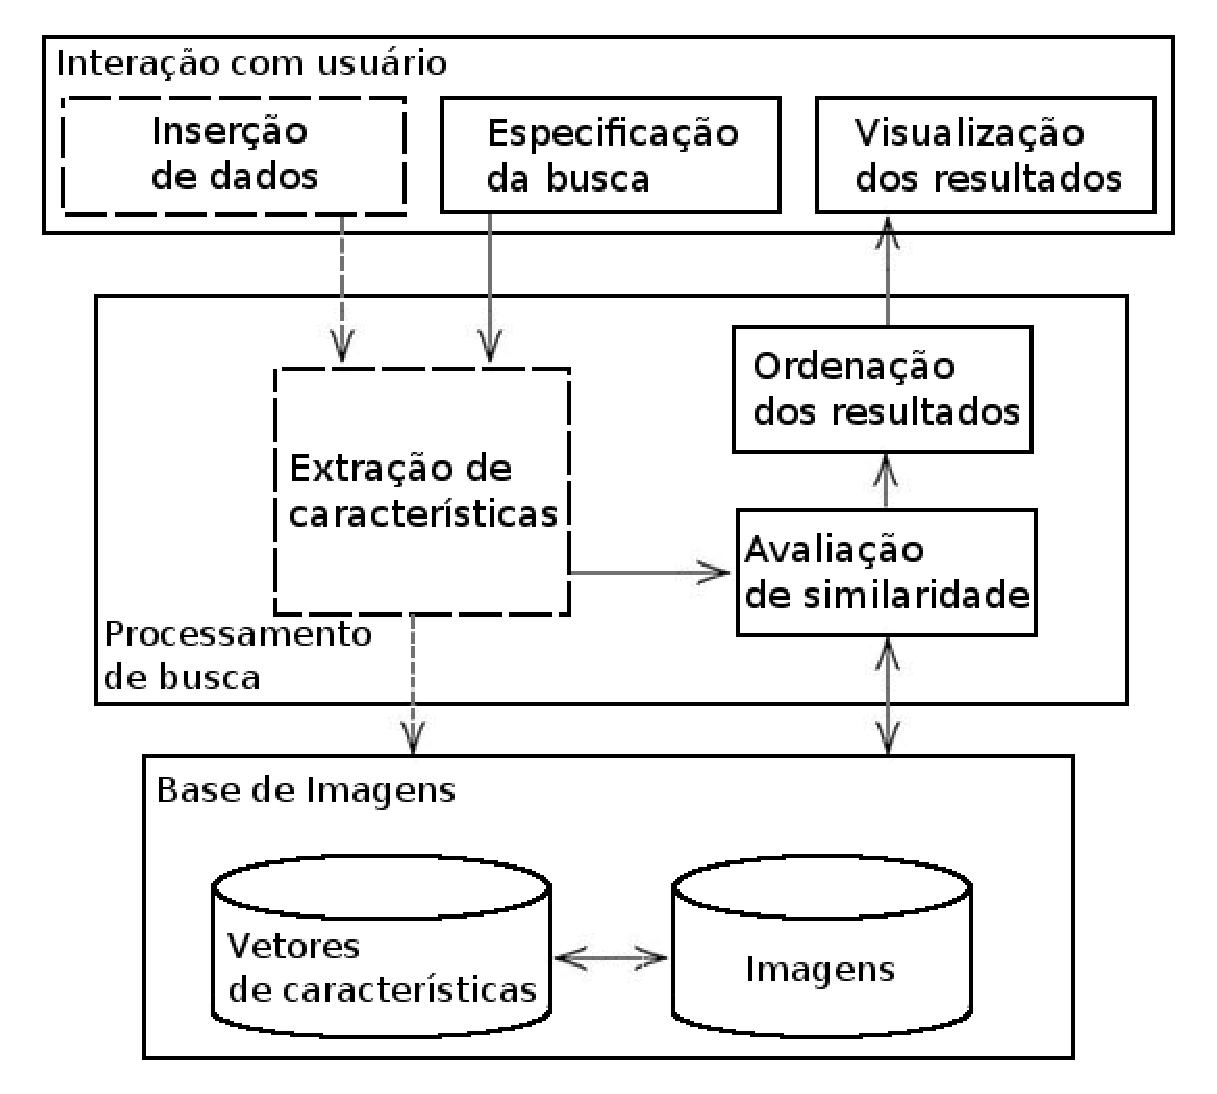
\includegraphics[width=0.65\textwidth]{cbir.eps}
\legend{Fonte: \citeonline{Torres:2006}.}
\end{figure}
 
Neste trabalho enfatizamos os processos de extração de características e de avaliação de similaridade em \emph{CBIR}, sendo esses processos destacados nas subseções a seguir.

\subsection{Extração de características}

O processo de extração de características das imagens forma é fundamental para os sistemas \emph{CBIR}. Tal processo se dá através de operações de processamento de imagens, cujo objetivo é extrair informação que seja semanticamente relevante dos atributos da imagem para a realização das buscas por similaridade de conteúdo. Os atributos comumente empregados para extração de características em \emph{CBIR} são a cor, a textura, a forma e a localização espacial dos elementos constituintes de uma imagem. 

A cor é o atributo mais empregado em \emph{CBIR}, pois a mesma permite discriminar uma ampla gama de imagens. Quando se utiliza esse atributo deve se considerar que o registro da cor em uma imagem varia consideravelmente com a orientação da superfície imageada, o posicionamento da câmera, a posição da fonte de iluminação e a maneira como a luz interage com os objetos imageados \cite{Smeulders:2000}. Ademais, a percepção humana da cor é um assunto complexo que ainda não está completamente elucidado \cite{Smeulders:2000}. De acordo com \citeonline{Torres:2006}, as técnicas de descrição por cores podem ser agrupadas em duas grandes classes dependendo se a informação de cor é codificada correlacionada com a sua distribuição espacial ou não. 

\begin{comment}Esses mesmos autores exemplificam como técnicas que não levam em consideração a distribuição espacial das cores os histogramas e os momentos de cores. 
\end{comment}

Atributos de textura são úteis na recuperação de imagens de satélites, bem como na busca de documentos digitalizados \cite{Smeulders:2000}. A textura é definida em termos de estruturas formadas por grupos de pixels que aparecem na imagem com certa periodicidade ou aleatoriedade. O método já consagrado para descrição de características de texturas é a matriz de coocorrência proposta por \citeonline{4309314}. No entanto, métodos baseados em transformações wavelet têm sido utilizados \cite{5376587}, mais notoriamente a transformada wavelet de Gabor \cite{531803}. Outra técnica que tem sido explorada na atualidade para descrição de texturas é a dimensão fractal multiescala \cite{Florindo:2013}. 

Informação relativa à localização espacial dos elementos de uma imagem permite, por exemplo, recuperar imagens de cenas fotográficas de paisagens externas, aonde distingue-se a localização do céu na região superior da imagem. Ademais, imagens fotográficas também tendem a apresentar em seu centro alguma informação significativa que difere do entorno da imagem, sendo essa informação útil no processo de recuperação de imagens de fotografias de pessoas, animais, etc.

A forma é uma característica intrínseca das imagens que é amplamente explorada pelo sistema de visão dos primatas para o reconhecimento de objetos. Progressos significativos têm sido alcançados no desenvolvimentos de sistemas de recuperação de imagens pelo conteúdo baseados nesse atributo.

Dentre as abordagens empregadas na obtenção de representações a partir das formas, a mais popular é a que as representa através de vetores de características. Tal representação permite que a similaridade entre as formas seja avaliada através de medidas de distância entre vetores. No entanto, a representação por vetores de características é pouco discriminativa, o que limita a sua acurácia em aplicações \emph{CBIR}.

Na representação estrutural, as formas são divididas em um conjunto de partes constituintes, sendo cada parte representada individualmente através de vetores de características. O descritor é composto a partir desses vetores e da relação existente entre as partes, representadas através de estruturas de dados como grafos, árvores ou cadeias de caracteres. Uma vez que esses métodos comparam as formas a partir das suas estruturas, esses conseguem uma boa acurácia, porém a um custo computacional elevado.

% {\color{red}Métodos de representação de formas por transformação empregam transformadas como wavelet, Fourier e Espaço-Escala para descrever as formasESTA PEDINDO PARA CITAR TRABALHOS AQUI, OU ENTAO ELIMINA. Em \emph{CBIR}, o custo computacional das buscas deve levar em consideração o custo de se aplicar a transformada à forma de consulta. }


O descritor do contorno da forma SC ou \emph{shape context} \cite{Belongie:2002} avalia a similaridade entre formas por correspondência de pontos. Esse descritor caracteriza a distribuição dos demais pontos do contorno em relação a um ponto de referência para cada ponto do contorno tomado como referência. 
Os métodos que usam correspondência, ou alinhamento, representam as formas diretamente no domínio espacial. Esses métodos determinam o grau de similaridade entre duas formas tentando alinhá-las de modo a medir a diferença residual existente entre as mesmas.


\begin{comment}
As abordagens empregadas na obtenção de representações a partir das formas podem ser classificadas em 3 grandes categorias:

\begin{alineas}

\item representação por vetor de características: É a técnica mais popular de representação. Neste método, a forma é representada através de um vetor numérico e a similaridade entre as formas é avaliada através de uma distância entre vetores. 

\item representação por transformação: deformações são realizadas em uma forma a fim de transformá-la em outra. A similaridade entre as formas é medida pelo esforço necessário para se realizar a transformação.  

\item representação relacional: Nesta abordagem as formas são divididas em um conjunto de partes constituintes. Cada parte é individualmente representada através de vetores de características. O descritor é composto a partir destes vetores e da relação existente entre as partes.
\end{alineas}

Técnicas de representação por vetores de características são classificadas em duas grandes classes: técnicas baseadas em região e técnicas baseadas em contorno.
\end{comment}

\subsection{Medidas de similaridade}
O processo de recuperação de imagens pelo conteúdo requer que alguma medida seja empregada na avaliação da similaridade entre as representações das imagens. Nas técnicas de extração de características que resultam em representações vetoriais, as medidas de distância entre vetores são comumente empregadas para este fim. Desta forma, o grau de similaridade entre duas representações guarda uma relação inversa com a medida de distância correspondente. 

 Uma medida entre dois vetores $p$ e $q$ é considerada uma distância quando satisfaz as seguintes propriedades \cite{Ullah1996}: 

\begin{alineas}
\item Positividade: $d(p,q) \geq 0$;  
\item Unicidade: $d(p,q) = 0 \Rightarrow p = q$;
\item Simetria: $d(p,q) = d(q,p)$;
\item Desigualdade triangular: $d(p,r) + d(r,q) \geq d(p,q)$.
\end{alineas}

Para as representações vetoriais dentro de um mesmo espaço dimensional, distâncias entre vetores, como as apresentadas na Tabela \ref{tbl:distance}, são empregadas. Casos aonde a representação das imagens resulta em descrições de dimensões distintas, técnicas mais elaboradas, que utilizam programação dinâmica, são necessárias. Dentre essas técnicas a \emph{DSW} (\emph{Dynamic space warping})\cite{Alajlan20117,{4815272}} tem sido empregada na avaliação de similaridade entre formas, a partir de assinaturas extraídas dos seus contornos. 

\begin{table}
\centering
\caption{\label{tbl:distance}Medidas de distância entre vetores}
\begin{tabular}[]{ll}
\hline
Medida de distância&Fórmula matemática\\
\hline
Distância de Minkowski&$d(x,y) = \Big[\sum\limits_{i=1}^{n}(x_i-y_i)^m\Big]^\frac{1}{m}$\\
Distância euclidiana&$d(x,y) = \Big[\sum\limits_{i=1}^{n}(x_i-y_i)^2\Big]^\frac{1}{2}$\\
Distância city-block&$d(x,y)= \sum\limits_{i=1}^{n}|x_i-y_i|$\\
Distância Chebyshev&$d(x,y)= \max\limits_{i}|x_i-y_i|$\\
Separação angular&$d(x,y)=\frac{\sum\limits_{i=1}^n{x_iy_i}}{\Big[\sum\limits_{i=1}^n{x_i^2}\sum\limits_{i=1}^n{y_i^2}\Big]^\frac{1}{2}}$\\
Canberra&$d(x,y) = \sum\limits_{i=1}^n\frac{|x_i-y_i|}{x_i+y_i}$\\
\hline
\end{tabular}
\end{table}

\section{\label{chap:contour}Descritores do contorno das formas}

Os estímulos visuais, ao qual os sistemas de visão biológicos estão submetidos, apresentam um elevado grau de redundância de informação. No processamento dessa informação, tais sistemas buscam eliminar essas redundâncias, retendo apenas a quantidade de informação necessária para o desempenho da tarefa requerida.  

Em visão computacional e reconhecimento de padrões, dá-se o nome a esse processo de eliminação das redundâncias de extração de características. Esta etapa de baixo nível busca encontrar informação relevante em uma imagem e representá-la convenientemente para a realização de uma tarefa específica de visão computacional. Uma vez que o processo de extração de características determina o desempenho de um sistema de visão computacional, este recebe especial atenção no desenvolvimento de tais sistemas.

Dentre os atributos dos quais se realizam a extração de características, a forma é considerada a mais relevante em diversas aplicações de visão artificial pela riqueza de informações que esta possui. Uma forma é obtida quando um objeto de interesse é identificado e segmentado em uma imagem. 
 De acordo com \citeonline{Zhang:2004}, para que se obtenha uma representação conveniente com base nesse atributo, deve-se buscar por informações que tenham importância em sua percepção, seja no contorno ou na região que a delimita. 

Obter uma representação, ou descrição, de objetos a partir de formas planas é uma tarefa complexa. Isso porque quando projetamos os objetos tridimensionais do mundo real em duas dimensões, perdemos as informações de uma das dimensões. Como resultado temos uma representação bidimensional parcial do objeto projetado. O problema torna-se ainda mais complexo se levarmos em conta que a forma é frequentemente corrompida por ruídos, defeitos, distorções arbitrárias e oclusões.

\citeonline{Zhang:2004} classificam as técnicas de representação de formas em duas grandes classes de métodos: os baseados em contorno e os baseados em região. Nos métodos baseados em região as características são extraídas de toda região da forma, enquanto que nos métodos baseados em contorno, as características são extraídas apenas da borda. Os referidos autores ainda subdividem cada classe de métodos em métodos estruturais e globais. Essa subdivisão é baseada em se a forma como um todo é utilizada na representação ou se a representação é obtida de partes, segmentos e seções das formas. 

A Figura \ref{fig:folha_contorno1} ilustra as etapas envolvidas no processo de representação de uma forma. Temos nesse caso a segmentação da imagem por limiar seguida da extração do contorno. Com base no contorno, obtém-se uma variedade de representações, na forma de sinais, adequadas para as tarefas de comparação, classificação e reconhecimento de formas.

Neste trabalho  enfatizamos a aplicação de técnicas de processamento de sinais para a obtenção de representações globais do contorno das formas, uma vez que tais técnicas têm sido empregadas com sucesso para esse propósito \cite{Costa:2009}. 

\begin{comment}
Técnicas baseadas em contorno de formas exploram apenas a região da borda da forma. Há dois tipos de abordagens para extração de características do contorno das formas: global e estrutural. Na abordagem global a forma não é dividida em subpartes e um vetor de características que representa toda a borda é obtido para representar a forma. Na abordagem estrutural a borda da forma é particionada em segmentos, denominados de primitivas mediante algum critério. A representação final é geralmente uma cadeia de caracteres, um grafo ou uma árvore.
\end{comment}



%representar uma forma consiste em caracterizá-la através de um conjunto de características que permitam reconstrui-la exatamente ou com um certo grau de precisão. Os mesmos autores classificam os métodos de representação das formas em três grandes grupos: por contorno, por região e por transformação.
    

\begin{figure} 
\caption{\label{fig:folha_contorno1} Obtenção da forma e do contorno da imagem de uma folha.}
%\includegraphics[width=\textwidth,clip,trim=12mm 188mm 27mm 75mm]{figura_folha.png}
\includegraphics[width=\textwidth,clip,trim=10mm 145mm 36mm 26mm]{figura_folha_v3.png}
%\legend{Fonte: próprio autor}
\end{figure}

\subsection{\label{sec:Assinatura}Representação paramétrica do contorno e curvatura
}

\citeonline{Costa:2009} definem assinatura de uma forma como sendo um sinal discreto unidimensional que descreve algumas das características do seu contorno ou da sua região. Devido a redução de dimensionalidade, as assinaturas do contorno são representações compactas das formas. Estas assinaturas podem ser utilizadas diretamente como descritores, porém o custo computacional envolvido em sua comparação direta é elevado. Isso porque as assinaturas, em geral, não são totalmente insensíveis a rotação, translação e escalamento das formas, bem como variam no total de amostras conforme varia a resolução das imagens. Algumas assinaturas são mais sensíveis a ruído e a pequenas distorções dos contornos, tornando necessário realizar filtragens. Embora melhore a robustez, tal processo acarreta em alguma perda de informação.

% Várias assinaturas vêm sendo empregadas na literatura para descrição de formas nas mais diversas aplicações, tais como a distância ao centroide, as coordenadas complexas, ângulo tangente, ângulo acumulativo, curvatura, área e comprimento da corda \cite{Zhang:2004}.

% \subsubsection*{\label{sec:Rep_par}Coordenadas paramétricas}
A representação por coordenadas paramétricas consiste na otenção das coordenadas dos pontos amostrados do contorno, representados a partir de um sistema de coordenadas preestabelecido, percorrendo-o sequencialmente em sentido horário ou anti-horário. Para o contorno discreto $\mathbf{C}$, com $N$ amostras, representado num sistema de coordenadas cartesianas, tal processo origina um conjunto de tuplas $\mathbf{C}[n] = \big(\mathbf{x}[n]\:\text{,}\:\mathbf{y}[n]\big)$, $n \in {\{0\:\text{,}\:1\:\text{,}\:\dotsc\:\text{,}\:N-1\}}$, cujas componentes $\mathbf{x}[n]$ e $\mathbf{y}[n]$ são sinais discretos vetoriais das coordenadas amostradas do contorno.

Na Figura \ref{fig:folha_contorno} estão representados os sinais obtidos para o contorno da folha da Figura \ref{fig:folha_contorno1} com a amostragem $N = 280$ pontos. Em vermelho está destacado o ponto de origem aonde a varredura, em sentido horário, se inicia. Os dois pontos observados aonde a evolução do sinal $\mathbf{x}[n]$ inverte sua tendência (de crescente para decrescente e de decrescente para crescente) correspondem aos pontos mais salientes da folha. Já o platô observado no sinal $\mathbf{y}[n]$ corresponde a região da parte inferior da folha, em que quase não se observa variações do contorno ao longo do eixo $Y$.
   
\begin{figure} 
\caption{\label{fig:folha_contorno} Processo de obtenção da representação paramétrica do contorno da folha da Figura \ref{fig:folha_contorno1}.}
\includegraphics[width=\textwidth,clip,trim= 12mm 30mm 10mm 77mm]{figura_folha_v3.png}
%\legend{Fonte: próprio autor}
\end{figure}

Outra representação paramétrica para o contorno é obtida compondo-se um sinal complexo $\mathbf{z}[n] = \mathbf{x}[n] + j\mathbf{y}[n]$, $j = \sqrt{-1}$, $n \in {\{0\:\text{,}\:1\:\text{,}\:\dotsc\:\text{,}\:N-1\}}$. Essa representação é conveniente quando se deseja realizar extração de características do contorno através de operações de processamento de sinais. A Figura \ref{fig:folha_complex} ilustra o módulo e a fase da representação complexa do contorno da folha da Figura \ref{fig:folha_contorno1}. 

\begin{figure} 
\caption{\label{fig:folha_complex} Representação paramétrica do contorno da forma da folha na imagem da Figura \ref{fig:folha_contorno1} como sinal complexo.}
\centering
\includegraphics[width=0.75\textwidth]{folha_complex_v3.png}
%\legend{Fonte: próprio autor}
\end{figure} 

Embora sejam descritivas, as representações por coordenadas paramétricas apresentam o inconveniente de não serem invariantes a translação, rotação ou escalamento das formas, porém, outras assinaturas com tais propriedades podem ser derivadas a partir dessas mesmas \cite{Kindratenko:2003}.

% \subsubsection*{Curvatura\label{sec:curvatura}}

A curvatura é uma assinatura do contorno da forma com importantes propriedades geométricas, o que motiva sua utilização para obtenção de descritores. Há evidências biológicas de que as propriedades desta assinatura sejam exploradas pelo sistema de visão dos primatas nas tarefas de reconhecimento de formas \cite{Costa:2009}. Na Tabela \ref{tbl:curv} estão destacadas as principais propriedades que a curvatura apresenta.  

\begin{table}
\centering
\caption{\label{tbl:curv} Propriedades da curvatura e as características geométricas que essas representam.}
\begin{tabular}[]{ll}
\toprule
\multicolumn{1}{c|}{Propriedade} & \multicolumn{1}{c}{Característica da forma}\\ 
\hline
Máximo valor absoluto & Ponto saliente \\
Máximo valor positivo & Saliência convexa \\
Mínimo valor negativo & Saliência côncava \\
Valores constantes e nulos & Segmentos retilíneos \\
Valores constantes e não nulos & Segmentos circulares \\
Cruzamentos de zero & Pontos de inflexão \\ \bottomrule
\end{tabular}
\legend{Fonte: \citeonline{Costa:2009}}
\end{table}

A função curvatura ($K(l)$), para uma curva contínua fechada $C = \big(x(l)\:\text{,}\:y(l)\big)$,  cujo perímetro é $L$ e que encontra-se parametrizada em $l \in [0\text{,}L]$, é definida como sendo \cite{Kindratenko:2003}:

\begin{equation} \label{eq:curvatura}
K(l) = \frac{x^{'}(l)y^{''}(l)-x^{''}(l)y^{'}(l)}{((x^{''}(l))^{2}+(y^{''}(l))^{2})^{\frac{3}{2}}}\text{,}
\end{equation}

\noindent 
sendo $\big(x^{'}(l) \text{, }y^{'}(l)\big)$ e $\big(x^{''}(l)\text{ , }y^{''}(l)\big)$ as derivadas primeira e segunda das coordenadas paramétricas da curva, respectivamente.

Sob o aspecto computacional, o cálculo da curvatura do contorno de uma forma requer que o mesmo seja espacialmente amostrado e discretizado. Tal processo torna o cálculo das derivadas da Equação \ref{eq:curvatura} sensível ao ruído e inviável, o que limita a aplicação direta da curvatura para a obtenção de descritores. 

A Figura \ref{fig:cir1} ilustra tal efeito para uma imagem de forma circular. A Figura \ref{fig:cir1}a representa o gráfico da curvatura teórica, obtida analiticamente, pela aplicação da Equação \ref{eq:curvatura} ao contorno parametrizado do círculo de mesmo raio ao do círculo da Figura \ref{fig:cir1}b. Já na  Figura \ref{fig:cir1}c, temos a curvatura obtida computacionalmente a partir do contorno discreto extraído do círculo da Figura \ref{fig:cir1}b. Nota-se que a curvatura da Figura \ref{fig:cir1}a (analítica) tem um valor constante $K(l) = \frac{1}{r}$, sendo $r$ o raio do círculo central, enquanto que a curvatura Figura \ref{fig:cir1}c (computacional) varia significativamente em torno do valor analítico esperado, como mostra a Figura \ref{fig:cir1}. 

\begin{figure}[h!]
  \caption{\label{fig:cir1} Efeito do ruído na estimativa computacional da curvatura para uma forma circular.}
  \centering
  \includegraphics[width=\textwidth, clip, trim=20mm 5mm 0mm 0mm]{curv_cir.png}
  %\legend{Fonte: próprio autor}
\end{figure}

Diversas estratégias foram propostas na literatura para contornar o problema da sensibilidade ao ruído do cálculo computacional da curvatura. Trabalhos clássicos, como os de \citeonline{5009188} e \citeonline{LynnBeus1987291} estimam a curvatura a partir do ângulo formado entre vetores obtidos a partir dos pontos do contorno. \citeonline{Cazals:2003} e \citeonline{Shi20022051} apresentaram trabalhos que utilizavam métodos para estimação da curvatura por interpolação de pontos. 

\citeonline{149591} introduziram um método que suaviza o contorno, através da convolução do mesmo com um filtro gaussiano, antes de se calcular a curvatura.

\begin{figure}[h!]
 \caption{\label{fig:curv_folha} Curvatura estimada do contorno da folha da Figura \ref{fig:folha_contorno1} através de método computacional.}
  \centering
  \includegraphics[width=0.75\textwidth]{curv_folha_v2.png}
%\legend{Fonte: próprio autor}
\end{figure}

A Figura \ref{fig:curv_folha} mostra a curvatura estimada, para o contorno da folha da Figura \ref{fig:folha_contorno1}, através do método proposto por \citeonline{149591}. O contorno foi previamente suavizado com um filtro gaussiano com desvio padrão $\sigma = 20$. Os pontos aonde a curvatura apresenta os picos em destaque correspondem aos pontos salientes da folha. 

\begin{comment}
Particularmente, métodos de extração de características multiescala do contorno a partir da curvatura conseguem superar o problema supracitado aplicando filtragens passa-baixa a representação paramétrica do contorno antes de se calcular a curvatura. 
\end{comment}

% {\color{magenta}
% \subsubsection*{Distância ao centroide}
% Uma assinatura simples pode ser obtida calculando-se a distância de cada coordenada do contorno ao centroide da forma. Esse último consiste, para um contorno discreto de $N$ amostras, em um vetor calculado, a partir das coordenadas do contorno, pela seguinte equação: 

% \begin{equation}
% \big(x_{c}\:\text{,}\:y_{c}\big) = \Big(\frac{1}{N}\sum^{N}_{i=0}{\mathbf{x}[i]}\:\text{,}\:\frac{1}{N}\sum^{N}_{i=0}{\mathbf{y}[i]}\Big)\text{.}
% \end{equation}

% O sinal da distância ao centroide $\mathbf{dc}[n]$ é dado por:

% \begin{equation}
% \mathbf{dc}[n] = \sqrt{(\mathbf{x}[n] - x_c)^2 + (\mathbf{y}[n] - y_c)^2}\text{.}
% \end{equation}

% Essa assinatura tem a propriedade de ser invariante a translação da forma, o que a torna independente do sistema de coordenadas adotado na parametrização do contorno. Embora não seja invariante a escala e a rotação, tais invariâncias podem ser obtidas, como sugerem alguns trabalhos. 

% Empregando um processo de subamostragem e de normalização pelo maior valor, \citeonline{Wang:2000} tornam essa assinatura invariante a escala. Para se alcançar invariância a rotação os referidos autores sugerem que, no processo de avaliação de similaridade entre duas assinaturas, seja realizado o deslocamento cíclico de uma das assinaturas até que se obtenha a maior similaridade.

% Já \citeonline{Zhang:02} utilizam a distância ao centroide como assinatura para se obter os descritores de Fourier. Tal estratégia garante as propriedades de invariância a rotação e a escala.

% \begin{figure}[h!]
%   \caption{\label{fig:cd} Assinatura da distância ao centroide para o contorno da folha da Figura \ref{fig:folha_contorno1}}
%   \centering
%   \includegraphics[width=0.75\textwidth]{cd_v2.png}
%   %\legend{Fonte: próprio autor}
% \end{figure}

% A Figura \ref{fig:cd} ilustra a assinatura da distância ao centroide para a folha da Figura \ref{fig:folha_contorno1}. Neste exemplo, a assinatura foi normalizada a partir da distância máxima ao centroide, que corresponde ao ponto vermelho demarcado tanto no gráfico como no contorno. 

% \subsubsection*{Sequência de ângulos}

% A assinatura de sequência de ângulos é obtida a partir do ângulo formado entre vetores construídos a partir das coordenadas do contorno parametrizado conforme ilustrado na Figura \ref{fig:angulo}. 

% Para um dado ponto pertencente ao contorno, de coordenadas $(x_i\:\text{,}\:y_i)$, obtemos os vetores $\overrightarrow{v_1}$ e $\overrightarrow{v_2}$. O primeiro vetor é formado pela diferença entre as coordenadas $(x_i\:\text{,}\:y_i)$ e $(x_{i-p}\:\text{,}\:y_{i-p})$, enquanto o segundo vetor é formado pela diferença entre as coordenadas $(x_{i+p}\:\text{,}\:y_{i+p})$ e $(x_i\:\text{,}\:y_i)$. 

% Da propriedade do produto interno, temos a seguinte relação dessas coordenadas com o ângulo $\theta_i$, formado entre os vetores $\overrightarrow{v_1}$ e $\overrightarrow{v_2}$:

% \begin{equation}
% \overrightarrow{v_1}. \overrightarrow{v_2} = |\overrightarrow{v_1}||\overrightarrow{v_2}|\cos{\theta_i}=(x_i-x_{i-p})(x_{i+p}-x_i)+(y_i-y_{i-p})(y_{i+p}-y_i)\text{.}
% \end{equation}

% Logo, o ângulo $\theta_i$ é calculado através da seguinte expressão:

% \begin{equation}
% \theta_i = \arccos{\Big[\frac{(x_i-x_{i-p})(x_{i+p}-x_i)+(y_i-y_{i-p})(y_{i+p}-y_i)}{\sqrt{\big[(x_i-x_{i-p})^2+(y_i-y_{i-p})^2\big]\big[(x_{i+p}-x_i)^2+(y_{i+p}-y_i)^2\big]}}\Big]}\text{.}
% \end{equation}

% O parâmetro $p$ controla a sensibilidade da assinatura a características locais do contorno. Valores grandes desse parâmetro resultam em uma assinatura menos sensível a características locais, enquanto que valores pequenos fazem com que a assinatura seja mais sensível a características locais.  Em \cite{Fotopoulou:2013} essa assinatura foi empregada para identificação de espécies vegetais a partir do contorno das folhas.

% \begin{figure}[h!]
%   \caption{\label{fig:angulo} Ilustração geométrica do método de obtenção da assinatura de sequência de ângulos.}
%   \centering
%   \includegraphics[width=0.2\textwidth]{angulo.png}
%   %\legend{Fonte: próprio autor}
% \end{figure}

% \subsubsection*{Invariantes integrais}

% Uma vez que as assinaturas obtidas através de operadores diferenciais são sensíveis a ruídos e a pequenas deformações do contorno, \citeonline{Manay:2006} propuseram os invariantes integrais como uma representação inerentemente robusta a estes artefatos.

% Seja $C \subset \mathbb{R}^2$ um contorno fechado e $\overline{C}$ sua área interior.
% A função 

% \begin{equation}
%  B_r(p,x) = \left\{
%   \begin{array}{l l}
%     1 & \quad |p-x|\leq r\\
%     0 & \quad |p-x|> r
%   \end{array} \right.
% \end{equation} 

% \noindent
% indica se um ponto $x$ pertence ou não ao interior de um disco $B_r$,  centrado em $p$ e de raio $r$.

% Empregando a função acima especificada, obtém-se uma assinatura invariante integral através da seguinte equação: 

% \begin{equation}
% A(p) = \int_{\overline{C}}{B_r(p,x)dx}\text{,}
% \end{equation} 

% \noindent
% sendo $p \in [0,L]$ e $L$ o perímetro do contorno.

% A Figura \ref{fig:Aii} ilustra, do ponto de vista geométrico, o processo de obtenção da assinatura invariante integral. O disco $B_r(p)$ é centrado em cada ponto $p(s)$ pertencente ao contorno e a área de interseção entre $B_r(p)$ e a região interna ao contorno $\overline{C}(s)$ é determinada.

% \begin{figure}[h!]
%   \caption{\label{fig:Aii} Ilustração geométrica do método de obtenção da assinatura invariante integral.}
%   \centering
%   \includegraphics[width=0.75\textwidth, clip, trim = 0mm 55mm 0mm 40mm]{aii.png}
%   \legend{Fonte: \citeonline{Manay:2006}.}
% \end{figure}}

\subsection{Representações multiescala\label{chap:multiescala}} 

Qualquer método que se proponha a descrever características das formas com base em contornos deve ser capaz de representá-las de forma confiável e precisa. 

\begin{comment}Segundo \citeonline{149591}, esses devem satisfazer os seguintes requisitos:

\begin{alineas}
\item Invariância: duas curvas que tenham a mesma forma devem ter a mesma representação;
\item Unicidade: duas curvas que não tenham a mesma forma devem apresentar diferentes representações;
\item Estabilidade: pequenas variações observadas entre duas curvas devem resultar em pequenas variações em suas representações;
\item Eficiência: uma vez que alguns sistemas de visão computacional apresentam requisitos de tempo real, a descrição deve ser computacionalmente eficaz, demandando poucos recursos de memória e de processamento;
\item Fácil implementação: é recomendável que os métodos de descrição sejam simples e de fácil implementação de modo a requerer menos tempo de implementação e depuração; 
\item Relação com propriedades específicas das formas: o método de descrição deve ser capaz de representar propriedades das formas que este descreve.
\end{alineas}

Os referidos autores afirmam que muitos dos métodos de extração encontrados em visão computacional falharam em satisfazer um ou mais dentre estes requisitos.
\end{comment}

Embora carregue grande parte da informação a respeito das formas, o contorno é  sensível a ruídos, oclusões e variações das formas.  Em outros casos, o contorno não se apresenta completamente disponível, com regiões disjuntas e descontinuidades. Tais aspectos comprometem a confiabilidade e a precisão das assinaturas baseadas em contorno.  

A descrição multiescala do contorno das formas vêm se mostrando uma alternativa viável para superação de tais problemas. Esta técnica se baseia no método proposto por \citeonline{Witkin:1983} e \citeonline{Koenderink:1984} para análise de sinais em vários níveis de resolução. Esses autores introduziram o conceito de fator de escala, cujo ajuste determina o grau de resolução na qual ocorre a análise do sinal. 

Perante outros métodos, a grande vantagem da representação multiescala é a sua habilidade em representar os atributos das formas em vários níveis de detalhes, variando de escalas de baixa resolução, aonde os detalhes que diferenciam as formas de uma mesma classe não são levados em consideração, até escalas de alta resolução aonde esses detalhes são preservados \cite{Ullman:1996}.

\begin{figure}[h!]
  \caption{\label{fig:ms} Método de análise multiescala a partir da assinatura do contorno de uma forma.}
  \centering
  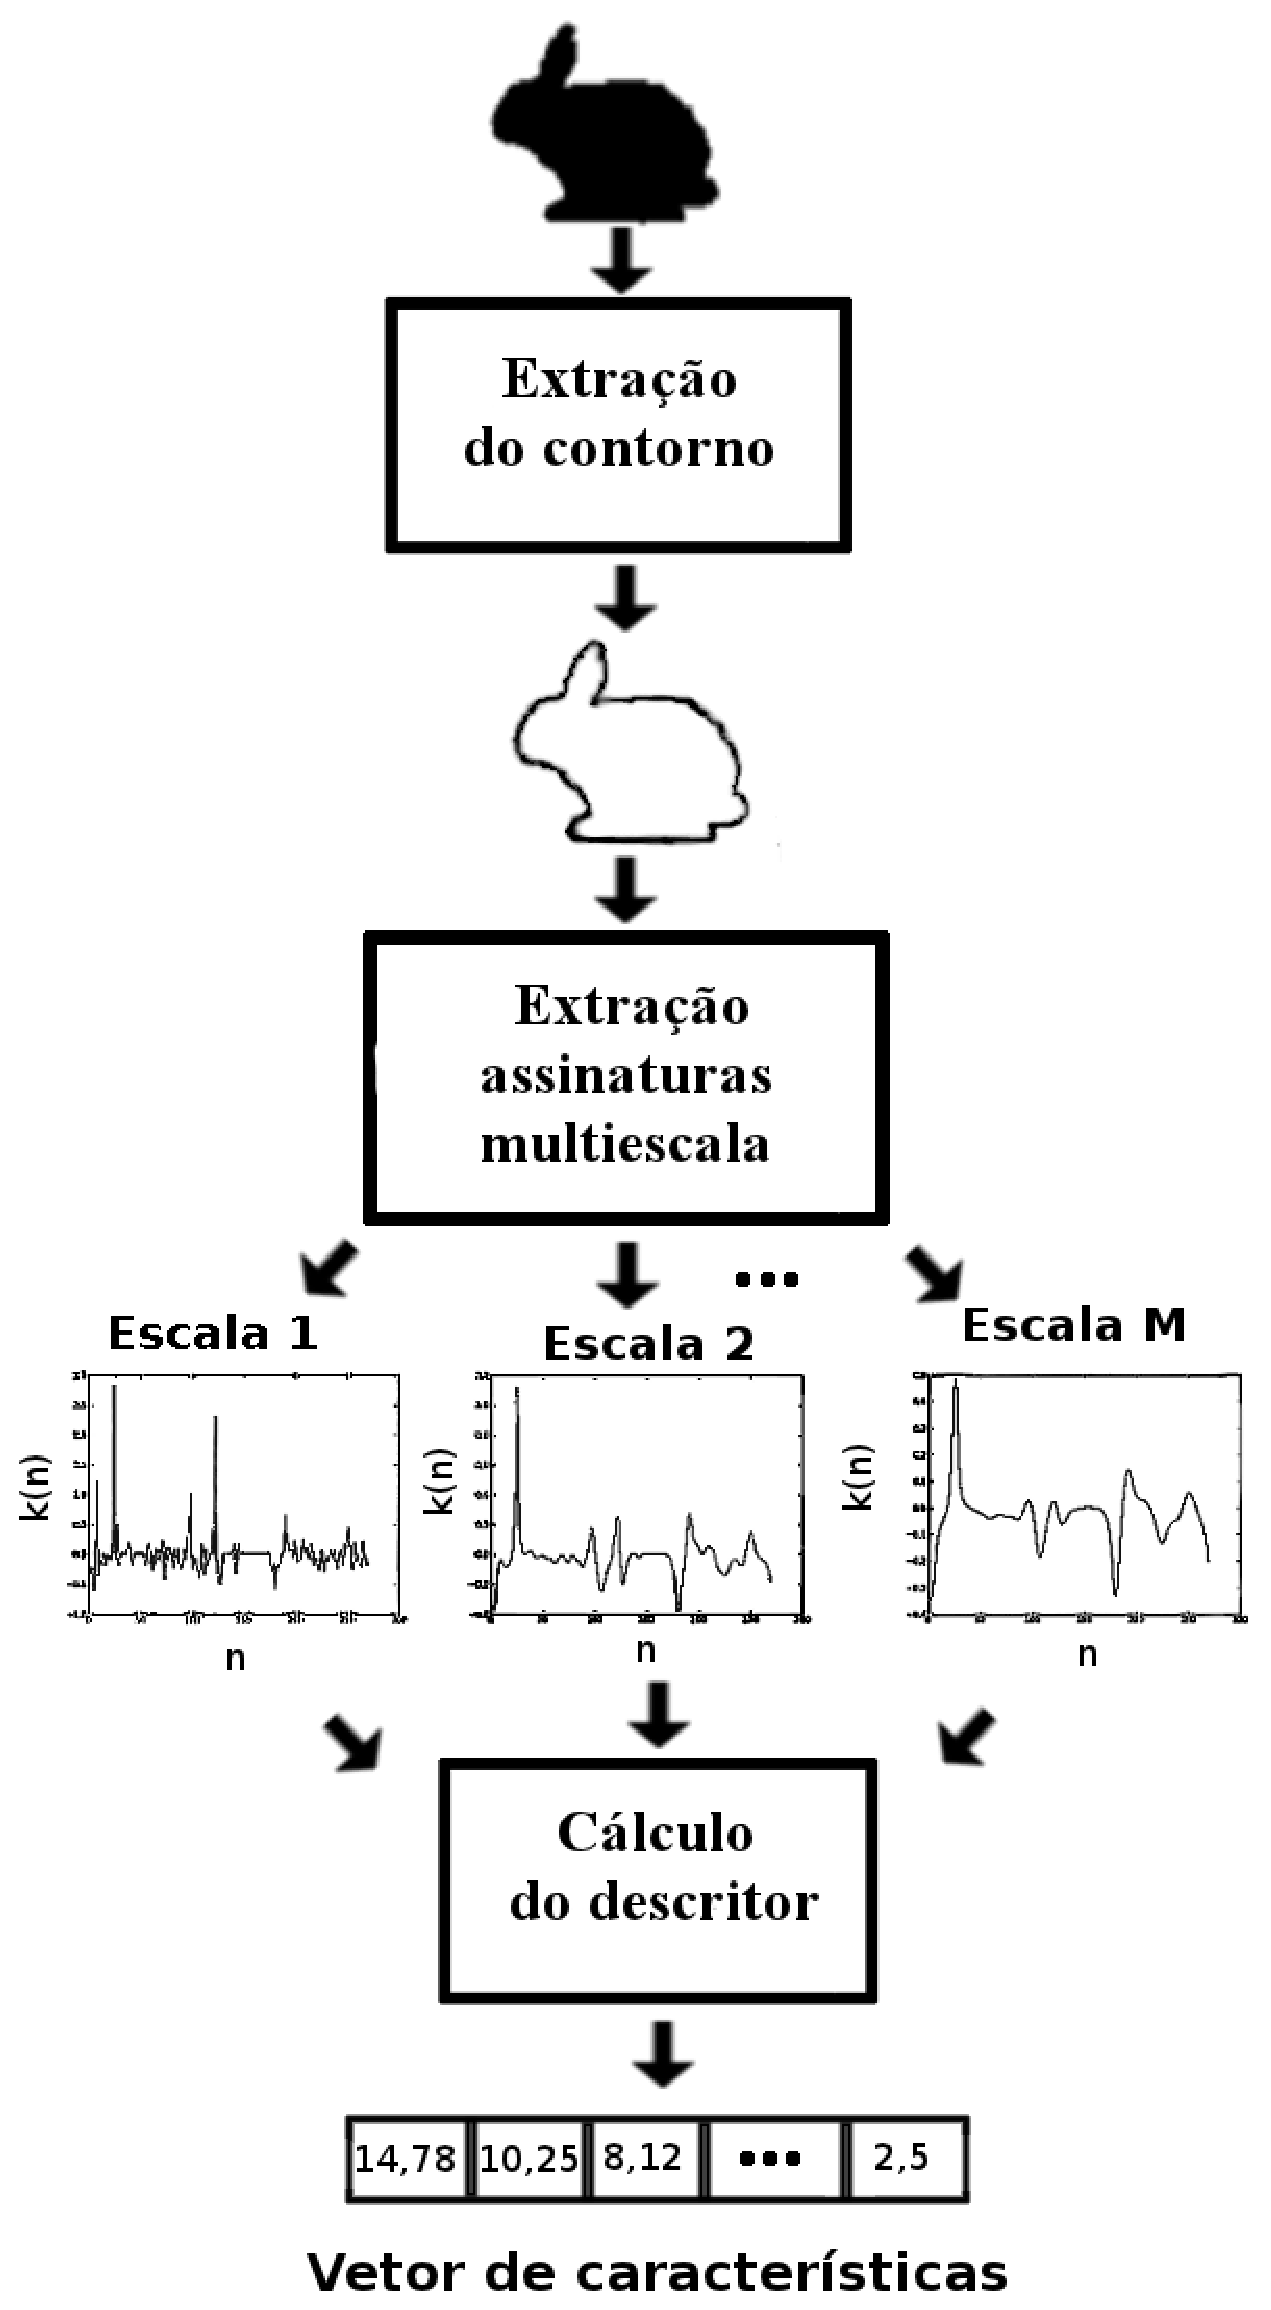
\includegraphics[width=0.45\textwidth]{feature_extraction.eps}
 % \legend{Fonte: próprio autor}
\end{figure}

A Figura \ref{fig:ms} ilustra o processo para obtenção de uma representação multiescala de um sinal unidimensional discreto $k[n]$ que represente o contorno de uma forma, tal como as assinaturas apresentadas na Subseção \ref{sec:Assinatura}. Emprega-se nesse processo uma função de transformação $F[n,\sigma]$, geralmente com características de filtragem passa-baixas e com frequência de corte $\sigma$. Na função de transformação, a referida frequência de corte corresponde ao fator de escala na qual o sinal $k[n]$ será analisado. 

Para um vetor de escalas $\sigma = (\sigma_1\:\sigma_2\:\ldots\:\sigma_M) $, a representação multiescala consiste em um vetor de sinais $k[n,\sigma] = (k[n,\sigma_1]\:k[n,\sigma_2]\:\ldots\:k[n,\sigma_N])$, sendo cada termo $k[n,\sigma_i]$ obtido através de
\begin{equation}\label{eq:ms1}
k[n,\sigma_i] = F[n,\sigma_i]*k[n]\text{,}
\end{equation}

\noindent
 aonde o operador $*$ denota a convolução entre o sinal $k[n]$ e a transformação $F[n,\sigma_i]$.  Assim, cada elemento de $k[n,\sigma]$ corresponde ao sinal $k[n]$ analisado na escala $\sigma_i$.

No caso de curvas planas, a análise multiescala permite descrevê-las em vários níveis de detalhes e de abstração a partir de suas assinaturas, tornando a representação mais discriminativa que os métodos que empregam medidas quantitativas globais, como área, perímetro e compacidade, devido a sua robustez e estabilidade \cite{4756134}.    

\subsubsection*{Curvatura Multiescala\label{subsec:curvMS}}

Inspirados na técnica de \citeonline{Witkin:1983} e \citeonline{Koenderink:1984}, \citeonline{149591} propuseram um método para análise multiescala do contorno através da assinatura da curvatura. O referido método emprega como função de transformação um filtro passa-baixas gaussiano, $g_{\sigma}(l) = \frac{1}{\sigma\sqrt{2\pi}}e^{\frac{l^2}{2\sigma^2}}$, que suaviza o contorno antes do cálculo de sua curvatura. Nesse caso, o ajuste do desvio padrão da função gaussiana ($\sigma^2$) atua como fator de escala, regulando a largura de banda do filtro e o nível de suavização do contorno.

%Desta forma, o sinal da curvatura é obtido em múltiplas escalas uma vez que a suavização do contorno possibilita o cálculo das derivadas. 


No caso contínuo temos as coordenadas do contorno suavizado realizando a convolução entre as coordenadas do contorno parametrizado $C(l) = (x(l)\text{,}y(l))$ e o filtro gaussiano:  

\begin{equation}
x_{\sigma}(l) = x(l) * g_{\sigma}(l) = \int^{\infty}_{-\infty}{x(v)g_{\sigma}(l-v)}dv \text{ e}
\end{equation}
\begin{equation}
y_{\sigma}(l) = y(l) * g_{\sigma}(l)=\int^{\infty}_{-\infty}{y(v)g_{\sigma}(l-v)}dv
\end{equation}\text{.}

Para o cálculo das derivadas $x^{'}_{\sigma}(l)\text{, }y^{'}_{\sigma}(l)\text{, }x^{''}_{\sigma}(l) \text{ e }y^{''}_{\sigma}(l)$, necessárias para o cálculo da curvatura do contorno suavizado, temos, pelas propriedades da convolução, $x^{'}_{\sigma}(l) = x(l) * g^{'}_{\sigma}(l)\text{, }y^{'}_{\sigma}(l) = y(l) * g^{'}_{\sigma}(l)\text{, }x^{''}_{\sigma}(l) = x(l) * g^{''}_{\sigma}(l)\text{ e }
y^{''}_{\sigma}(l) = y(l) * g^{''}_{\sigma}(l)$.

O cálculo da curvatura do contorno suavizado $K_{\sigma}(l)$ se dá através da equação \ref{eq:curvatura}, substituindo-se $x^{'}(l)\text{, }\:y^{'}(l)\text{, }\:x^{''}(l)\:\text{ e }\:y^{''}(l)$ por $x^{'}_{\sigma}(l)\text{, }\:y^{'}_{\sigma}(l)\text{, }\:x^{''}_{\sigma}(l)\:\text{ e }\:y^{''}_{\sigma}(l)$, respectivamente, ou seja,

\begin{equation} \label{eq:curvatura_ms}
K_{\sigma}(l) = \frac{x_{\sigma}^{'}(l)y_{\sigma}^{''}(l)-x_{\sigma}^{''}(l)y_{\sigma}^{'}(l)}{((x_{\sigma}^{''}(l))^{2}+(y_{\sigma}^{''}(l))^{2})^{\frac{3}{2}}}\text{.}
\end{equation}

Uma outra abordagem utilizada para se calcular a curvatura multiescala, que foi proposta por \citeonline{Cesar:1996} e adotada nesta tese, opera com a representação do contorno no domínio da frequência. A partir da transformada de Fourier das coordenadas do contorno suavizado $X_{\sigma}(f) = F\big\{x_{\sigma}(l)\big\}$ e $Y_{\sigma}(f) = F\big\{y_{\sigma}(l)\big\}$. Os referidos autores calculam derivadas utilizando a propriedade da derivada da transformada de Fourier, ou seja:

\begin{equation}
x_{\sigma}^{'}(l) = F^{-1}\big\{2 \pi j f  X_{\sigma}(f)\big\}
\end{equation}

\begin{equation}
y_{\sigma}^{'}(l) = F^{-1}\big\{2 \pi j f  Y_{\sigma}(f)\big\}
\end{equation}

\begin{equation}
x_{\sigma}^{''}(l) = F^{-1}\big\{- (2 \pi f)^2 X_{\sigma}(f)\big\}
\end{equation}

\begin{equation}
y_{\sigma}^{''}(l) = F^{-1}\big\{- (2 \pi f)^2 Y_{\sigma}(f)\big\}
\end{equation}, aonde $F^{-1}\big\{X(f)\big\}$ denota a transformada de Fourier inversa do sinal $X(f)$.

\begin{comment}
\begin{equation}
X(f) = F\big\{x(l)\big\} = \int\limits^\infty_\infty x(l)e^{-2 \pi j f l}dl
\end{equation}

\begin{equation}
x(l) = F^{-1}\big\{X(f)\big\} \int\limits^\infty_\infty X(f)e^{2 \pi j f l}df
\end{equation}
\end{comment}

Na suavização do contorno no domínio da frequência, ao invés da convolução, realiza-se o produto dos sinais $X(f)$ e $Y(f)$ com a transformada de Fourier da expressão do filtro gaussiano:

\begin{equation}
X_\sigma(f) = X(f).G_\sigma(f)
\end{equation}

\begin{equation}
Y_\sigma(f) = Y(f).G_\sigma(f)
\end{equation}, sendo

\begin{equation}
G_\sigma(f) = F\big\{ g_{\sigma}(l)\big\} = e^{-2 \pi^2 f^2 \sigma^2}\text{.}
\end{equation}

\begin{figure}[h!]
  \caption{\label{fig:curv_ms} Curvatura multiescala do contorno da folha da Figura \ref{fig:folha_contorno1}.}
  \centering
  \includegraphics[width=0.75\textwidth]{curvograma_v2.png}
 \end{figure}

A Figura \ref{fig:curv_ms} ilustra a evolução do sinal de curvatura do contorno da folha da Figura \ref{fig:folha_contorno1} para diferentes níveis de suavização. Os picos da curvatura que se preservam nas escalas de baixa resolução correspondem às informações mais salientes do contorno, que o caracterizam globalmente. As informações de detalhes, que tendem a desaparecer nas escalas de baixa resolução e se preservam nas escalas de alta resolução, representam as características mais especificas do contorno.

{\color{blue}
\citeonline{Costa:1997} propuseram um método para o ajuste das escalas através das expressões

\begin{equation}
oct_l = (\sqrt{2})^l;\text{ }l = 1,\ldots,S
\end{equation} 
\noindent e
\begin{equation}
\sigma_l = \big(\frac{\sigma_{max} - \sigma{min}}{oct_{max}-\sqrt{2}}\big)(oct_l - \sqrt{2})+\sigma_{min}\text{,}
\end{equation}

\noindent aonde $S$ é o número de escalas, $l$ a l-ésima escala calculada $\sigma_{min} = \sigma_1$ a menor escala e $\sigma_{max} = \sigma_S$ a maior escala.
}
 
\subsubsection*{Dimensão Fractal multiescala (DFM)}

O conceito de fractal, introduzido por \citeonline{Mandelbrot:2000}, está intimamente relacionado com a auto-similaridade ou escala de uma forma, o que por sua vez estabelece a noção de dimensão fractal.

Tanto a dimensão fractal como a dimensão fractal multiescala permitem estimar a complexidade de uma forma \cite{Backes:2012}. Complexidade é uma propriedade importante das formas que informa quanto espaço uma determinada forma ocupa \cite{Costa:2009}. A dimensão fractal multiescala estima a complexidade da forma através de uma curva que representa as mudanças na complexidade à medida que a escala de visualização da forma varia \cite{Florindo:2012}.

Nesta tese o método empregado para estimar a dimensão fractal e a dimensão fractal multiescala é o método de Minkowski-Bouligand \cite{Costa:2009}. Este método dilata a forma sob análise utilizando como elemento estruturante um disco de raio $r > 0$, sucessivamente. A inclinação da interpolação linear da curva $\log{A(r)}$ versus $\log{r}$ determina a estimativa da dimensão fractal $D_f$, que é dada por:

\begin{equation}
D_f = 2 - \lim_{r \to 0}  \frac{\log{A(r)}}{\log{r}}.
\label{eq:df}
\end{equation}

A derivada da curva log-log, representada através de $N$ valores discretos de raios $r_i>0$, determina a dimensão fractal multiescala:

\begin{equation}
DFM = \big(D_f(t_1)\text{, }D_f(t_2)\text{, }\ldots\text{ , }D_f(t_N)\big), 
\label{eq:dfm}
\end{equation}

\noindent aonde  $D_f(t) = 2 - \frac{du(t)}{dt}$, $t = \log{r}$ e $u(t) = \log{A(t)}$.


\section{Técnicas de visualização de dados}

Um problema dos algoritmos empregados na extração de características, que foram abordados nesse capítulo é a elevada dimensionalidade da representação vetorial obtida. Além de dificultar compreender a organização dos dados, essa elevada dimensionalidade acarreta em maior complexidade do sistema computacional que deve lidar com essa informação. 

Através de técnicas de redução de dimensionalidade é possível gerar visualizações gráficas dos dados, o que permite compreender melhor sua estrutura. Ademais, tais técnicas removem informações redundantes e irrelevantes, reduzindo assim a complexidade da representação obtida.

Apresentamos neste capítulo duas técnicas de visualização de dados que foram empregadas neste trabalho na avaliação da capacidade discriminativa dos descritores do contorno de formas: a análise das componentes principais (\emph{PCA}) e o mapa auto-organizável de Kohonen (SOM).

%Essas técnicas foram aplicadas aos descritores energia de dobramento multiescala, dimensão fractal multiescala, entropia diferencial multiescala e entropia discreta multiescala. Limitamos esse estudo a tais descritores porque os mesmos representam as formas através de vetores de características de mesma dimensão, que é um requisito para a aplicação das técnicas de visualização estudadas.

%Essas técnicas tem em comum a propriedade de projetar os dados de dimensionalidade elevada em um espaço bidimensional. 

\subsection{Análise das componentes principais (PCA)}

\begin{figure}[h!]
  \caption{\label{fig:nuvem_pca} Projeções das três primeiras componentes principais dos vetores de características obtidos  a partir do descritor \emph{NMBE} e os vetores transformados através de \emph{PCA}.}
  \centering
  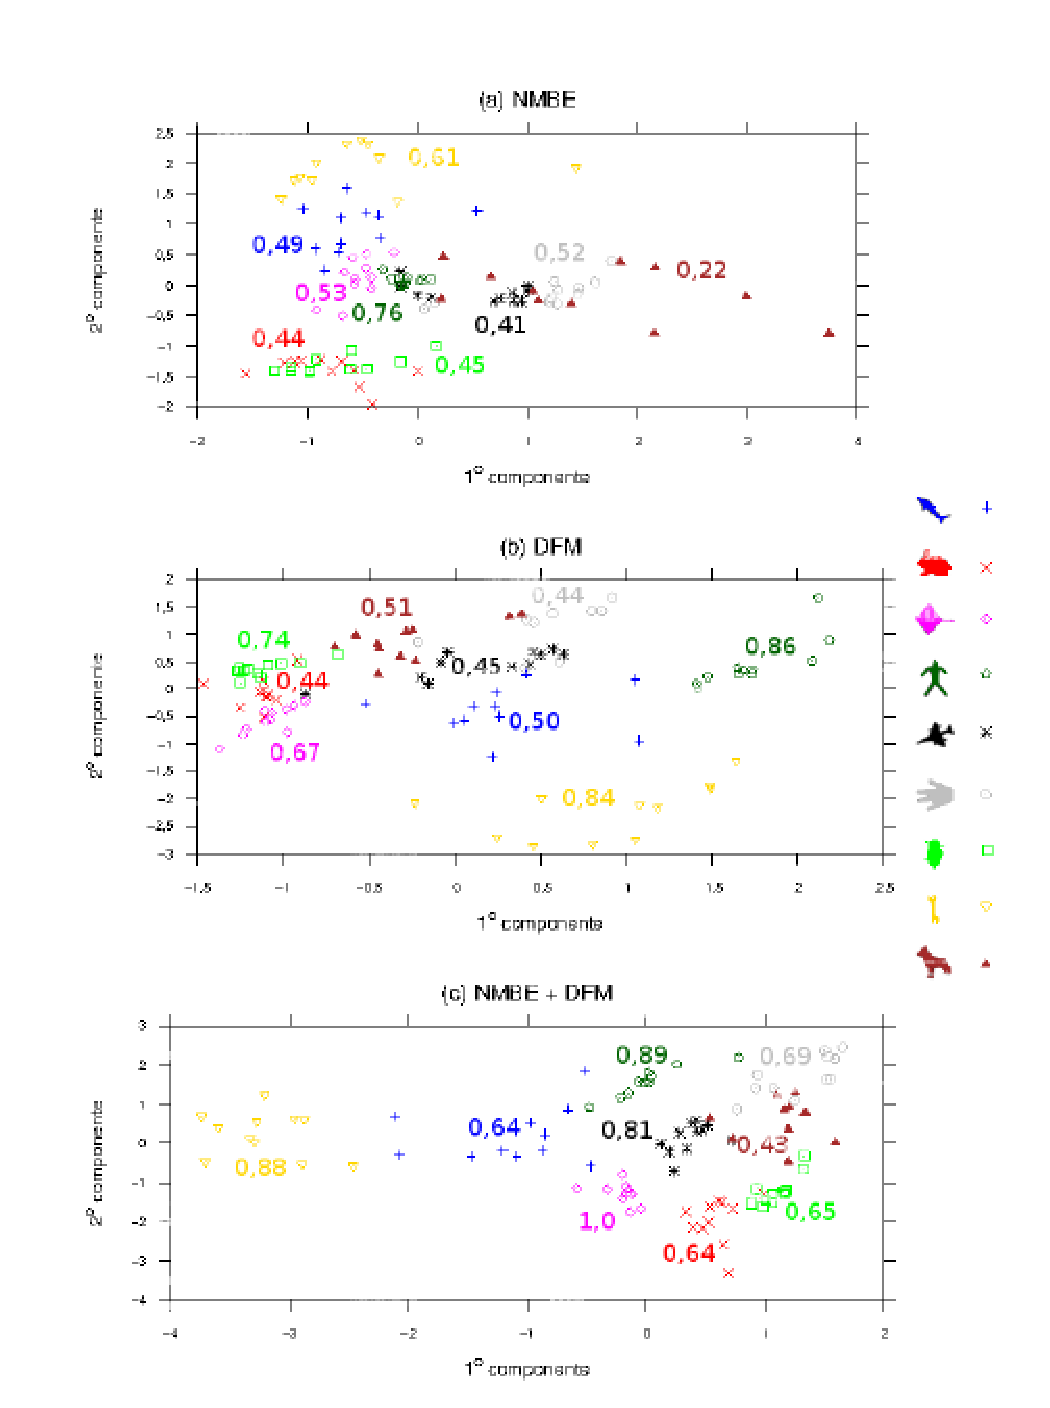
\includegraphics[width=0.75\textwidth]{nuvem_pca.eps}
\end{figure}

O propósito da análise das componentes principais é obter um conjunto de variáveis não correlacionadas, em ordem decrescente de importância, a partir da combinação linear das variáveis originais. Sob o aspecto geométrico, esse processo de combinar linearmente as variáveis pode ser entendido como realizar a rotação dos eixos do sistema de coordenadas original, a fim de se encontrar um novo sistema de coordenadas ortogonal em que as variáveis transformadas apresentem máxima variância. 

Desde que a maior parte da variância esteja concentrada nas primeiras componentes das variáveis transformadas, consegue-se obter através dessa técnica uma representação com um número reduzido de variáveis.

A técnica \emph{PCA} é não supervisionada, pois não leva em consideração informação a priori dos agrupamentos, ou rótulos, dos dados.  Sendo a transformação \emph{PCA} linear, temos que

\begin{equation}\label{eq:PCA1}
\mathbf{y}=\mathbf{A}^T\mathbf{x}
\end{equation}

\noindent aonde $ \mathbf{A} = \begin{pmatrix}
  a_{1,1} & a_{2,1} & \cdots & a_{p,1} \\
  a_{1,2} & a_{2,2} & \cdots & a_{p,2} \\
  \vdots  & \vdots  & \ddots & \vdots  \\
  a_{1,p} & a_{2,p} & \cdots & a_{p,p}
 \end{pmatrix} = 
 \begin{pmatrix}
 \mathbf{a_{1}}&
 \mathbf{a_{2}}&
 \cdots&
 \mathbf{a_{p}}
 \end{pmatrix}$ é a matriz de transformação, $\mathbf{x} = \begin{pmatrix} x_1&x_2&\ldots&x_p\end{pmatrix}^T$ e $\mathbf{y} = \begin{pmatrix}y_1&y_2&\ldots&y_p\end{pmatrix}^T$ vetores de variáveis aleatórias e $\mathbf{a_1}\text{ a }\mathbf{a_p}$ vetores dos coeficientes da base de transformação.
 
Logo, cada variável de saída $y_i$ é obtida através da combinação linear das variáveis de entrada pela seguinte equação:
 
 \begin{equation}\label{eq:PCA2}
 y_i = \sum\limits_{j = 1}^p a_{i,j}x_j = \mathbf{a_i}^T\mathbf{x}
 \end{equation}

Pode-se demonstrar que, para se obter em $\mathbf{y}$ variáveis que não são correlacionadas,  deve-se atribuir aos vetores de coeficientes $\mathbf{a_1} \ldots \mathbf{a_p}$ os auto-vetores da matriz de covariância de $\mathbf{x}$, sendo esta última dada por: 

\begin{equation}\label{eq:PCA3}
\mathbf{\Sigma_x} = E{[\mathbf{xx}^T]}-E{[\mathbf{x}]}E{[\mathbf{x}^T]}
\end{equation}

\noindent aonde $E[.]$ denota o operador esperança. 
Já que $\mathbf{\Sigma_x}$ é de dimensão $p \times p$, temos associada a esta $p$ auto-vetores ($\mathbf{a_1}\text{, }\mathbf{a_2}\text{, }\ldots\text{, }\mathbf{a_p}$) com $p$ auto-valores ($\lambda_1 > \lambda_2 \ldots > \lambda_p$) correspondentes, sendo cada auto-valor $\lambda_i$ a variância de cada variável de saída $y_i$ obtida através da Equação \ref{eq:PCA2}. 

Selecionando dentre as componentes somente aquelas de maior variância, que implica em construir a matriz de transformação apenas com os auto-vetores mais significativos, é possível obter uma representação dos dados em um espaço de dimensão reduzida e de mais fácil entendimento do ponto de vista geométrico.

Na Figura \ref{fig:nuvem_pca} temos representadas as projeções das duas componentes principais de maior variância para cada um dos descritores avaliados. Os valores numéricos correspondem a taxa de acerto média nos experimentos de recuperação de formas pelo conteúdo alcanças para cada classe de formas representada.

\subsection{Escalonamento multidimensional (\emph{MDS})}

O escalonamento multidimensional \cite{cox:2000} consiste em um método para representação de dados de um espaço inicial, multi dimensional, para um espaço de dimensão reduzida, preservando as relações de distâncias existentes no espaço inicial. Esse algoritmo modela a similaridade ou disimilaridade dos dados como distâncias no espaço geométrico.

Há dois tipos de algoritmos \emph{MDS}: o métrico e o não métrico. No primeiro, a matriz de similaridade de entrada é construída a partir de uma métrica de distância que respeita a desigualdade triangular. Assim, as distâncias entre dois pontos no espaço de dimensão reduzida são ajustadas para serem  mais próximas possível àquelas encontradas no espaço de dimensão inicial. Em sua versão não métrica, o algoritmo tenta preservar a ordem das distâncias, procurando uma relação monotônica não paramétrica entre as proximidades das distâncias do espaço de dimensão reduzida e as similaridades no espaço de dimensão inicial.

O coeficiente $R^2$ mede o ajuste da representação dos dados em um espaço de menor dimensão. Este coeficiente indica, em porcentagem, o ajuste do modelo aos dados observados. Assim, quando mais próximo de 1 o valor de $R^2$, melhor o ajuste do modelo aos dados observados.  Sejam $d$ e $\hat{d}$ as matrizes de distância simétricas entre dois vetores nos espaços de menor e maior dimensão, respectivamente. O coeficiente $R^2$ é dado por 
\begin{equation}
R^2= 1-\frac{\sum_{i=1}^n \sum_{j = i}^{n}(\hat{d}_{i,j} - d_{i,j})^2}{\sum_{i=1}^n\sum_{j=i}^n (d_{i,j}-\bar{d})^2}
\text{,}\:\: R^2 \in [0,1]
\end{equation}

\noindent em que  $n$ é o número de amostras, $d_{i,j}$ é a distância entre as amostras $i$ e $j$ no espaço de mais alta dimensão, $\hat{d}_{i,j}$ é a distância entre as amostras $i$ e $j$ no espaço de menor dimensão e $\bar{d}$  é a distância média no espaço de mais alta dimensão.



\subsection{Mapa auto-organizável de Kohonen}

O mapa auto-organizável de Kohonen, ou rede \emph{SOM} \cite{Kohonen:2001}, consiste em um tipo de rede neural de aprendizagem não supervisionada. Desenvolvida por \citeonline{Kohonen:1982}, a rede \emph{SOM} projeta os vetores apresentados em sua entrada de um espaço N-dimensional para um espaço bidimensional, preservando a estrutura topográfica do espaço vetorial de origem. Em outras palavras, se dois vetores encontram-se próximos no espaço de entrada, estes preservarão essa relação de proximidade no espaço de projeção. 

\begin{comment}
Em seu processo de treinamento, a rede \emph{SOM} agrupa os vetores de entrada através de um processo de aprendizado competitivo mantendo a estrutura topológica do espaço vetorial de entrada.
\end{comment}

Sendo uma ferramenta para análise exploratória de dados, esse tipo de rede neural tem sido empregada para visualização de imagens \cite{Strong2011774}, identificação de agrupamentos \cite{Kuroiwa200031}, classificação de texturas \cite{595364}, bem como outras aplicações.

\citeonline{Ultsch:1990} demonstraram que, embora a rede \emph{SOM} organize os vetores em agrupamentos, esta não representa as distâncias entre os mesmos de maneira fidedigna. Isso torna a análise direta do mapa de projeções não adequada para a análise dos agrupamentos estabelecidos. 

Para contornar esse problema, os referidos autores desenvolveram um método bidimensional de representação conhecido como matriz unificada de distâncias ou matriz-U. Obtida a partir do mapa \emph{SOM} essa matriz mostra, preservando a topologia, a relação de distância entre as estruturas mapeadas \cite{Ultsch:1990}. 

Para ilustrarmos como se interpreta a informação contida na matriz-U apresentamos como exemplo a imagem da Figura \ref{fig:u-matrix}. Nesta imagem a matriz-U é representada por um conjunto de células em níveis de cinza. As estruturas claras rotuladas representam os neurônios da rede SOM, enquanto as demais células representam o grau de separação existente entre as estruturas. Células mais escuras representam maior grau de separação entre as estruturas mapeadas pela matriz. Já células mais claras, tais como as que tendem ao branco, representam maior grau de proximidade entre as estruturas mapeadas. 

\begin{figure}[]
  \caption{\label{fig:u-matrix} Representação da Matriz-U como imagem em níveis de cinza. As células brancas rotuladas correspondem aos neurônios da rede SOM. Células escuras indicam maior separação entre neurônios e células claras indicam maior proximidade entre neurônios.}
  \centering
  \includegraphics[width=0.4\textwidth]{u-matrix_gray.png}
\end{figure}

Interpretando esta figura observamos que as estruturas A5, A4 e A8 estão bem próximas umas das outras. Já a estrutura A9 encontra-se afastada das referidas estruturas. Dada a grande separação existente entre as quatro estruturas analisadas e as demais estruturas da matriz (E8, E6, E10, E9, E3 e B9), podemos inferir que as quatro estruturas (A5, A4, A8 e A9) formam um agrupamento. Já as estruturas E8, E6, E10 e E9 formam um outro agrupamento, embora não estejam tão próximas umas das outras como no caso anterior. Quanto às estruturas B9 e E3, estas estão isoladas, ou seja, muito distante das demais estruturas da matriz.

\begin{comment}

The concept of fractal, introduced by Mandelbrot \citep{Mandelbrot:2000}, is closely related to self-similarity or scaling of a shape. Moreover, it encompasses the notion of fractional dimension.  Actually, fractal dimension and \emph{MFD} are well-known methods to estimate shape complexity \citep{Backes:2012}. Shape complexity is an important concept in shape analysis that informs how much space a shape occupies \cite{Costa:2009}. \emph{MFD} estimates shape complexity through a curve that represents changes in the complexity as the shape visualization scale varies \cite{Florindo:2012}. 

%and for feature extraction of biological forms %\citep{Rossatto:2011}.  In fact, it quantifies the %self-similarity of a shape.

% quantifica a aspereza ou rugosidade de uma forma \citep{Schroreder:1996}.\\

%Uma das caracter\'isticas das formas fractais \'e a sua auto-similaridade \citep{Schroreder:1996}. Isso significa que uma forma, tanto em escalas menores como maiores, \'e constitu\'ida por um mesmo conjunto de primitivas $D_f$.\\

%Qualquer forma auto-similar pode ser dividida em $N$ partes auto-similares, ou seja, c\'opias menores que sejam escalonadas por um fator $b$, atrav\'es da equa\c c\~ao:\\

%\begin{equation}
%D_{f} = \frac{\log{N}}{\log{\frac{1}{b}}}.
%\label{eq:dfc}
%\end{equation}

%Esse descritor pode ser construído a partir do método de Bouligand-Minkowski de estimação da dimensão fractal ($D_f$) \citep{Costa:2009}. Utilizado em \citep{Florindo:2012} e \citep{Backes:2012}, o referido método aplica dilatações exatas à  forma analisada tendo como elemento estruturante uma região circular de raio $r > 0$. O coeficiente angular da interpolação linear da curva $\log{A(r)}$ versus $\log{r}$ é utilizado como uma estimativa da $D_f$:

In this paper, the Minkowski-Bouligand method estimates the fractal dimension ($D_f$) \citep{Costa:2009} and hence the \emph{MFD} descriptor. This estimation method dilates the shape under analysis  using a disk structuring element of radius $ r>0 $, successively. The slope of the linear interpolation of the curve $\log{A(r)}$ versus $\log{r}$ provides the $D_f$ estimation, given by: 

\begin{equation}
D_f = 2 - \lim_{r \to 0}  \frac{\log{A(r)}}{\log{r}}.
\label{eq:df}
\end{equation}
%O cálculo da MFD decorre do calculo da derivada da curva log-log, obtida a partir da equação \ref{eq:df}, para diferentes valores de raios $r$:
Then, the derivative of th log-log curve for $N$ discrete values of radii $r_i>0$ gives 

\begin{equation}
MFD = \big(D_f(t_1)\text{, }D_f(t_2)\text{, }\ldots\text{ , }D_f(t_N)\big), 
\label{eq:dfm}
\end{equation}

\noindent where  $D_f(t) = 2 - \frac{du(t)}{dt}$, $t = \log{r}$ and $u(t) = \log{A(t)}$.

\end{comment}

\section{Métodos de otimização}

Problemas de otimização, que consistem em encontrar mínimo e máximo de uma função objetivo de múltiplas variáveis, ocorrem com frequência em diversas áreas do conhecimento, como engenharia, economia e ciências. Métodos clássicos,{\color{red} PRECISA CITAR UMA FONTE AQUI como o de Newton-Rapson }e suas variantes, funcionam muito bem no caso em que a função objetivo é diferenciável e com um único ótimo global no entanto, tais condições não são encontradas em diversos problemas. 

Os métodos de otimização evolutivos foram desenvolvidos para lidar com o problema de otimização de funções de múltiplas  variáveis, não diferenciáveis e com ótimos locais. Inspirados nos processos biológicos evolutivos, esses métodos utilizam de metaheurísticas e uma população de soluções candidatas para realizar buscas no espaço de pesquisa pela solução ótima. Esta seção apresenta três algoritmos metaheurísticos de otimização que foram utilizados nesta tese no ajuste de parâmetros dos descritores multiescala: evolução diferencial  \cite{Storn:1007}, enxame de partículas  \cite{Yuhui:1998} e recozimento simulado \cite{Andries:2007}.
%This paper investigates three optimization algorithms to search for the best solution that minimizes the objective function MAD: the simulated annealing (SA) \cite{Andries:2007}, differential evolution (DE) \cite{Storn:1007} and particle swarm (PSO) \cite{Yuhui:1998}. 
\subsection{Recozimento simulado (\emph{SA})}

O  recozimento simulado é um método clássico de otimização metaheurístico que simula o processo termodinâmico de aquecimento e resfriamento de um metal. O mecanismo desse método para exploração do espaço de busca consiste numa variável de temperatura que determina a probabilidade de aceitação de uma solução pior àquela encontrada até o momento, sendo que quanto maior for a termperatura, maior será essa probabilidade. Soluções melhores que a solução atual são sempre aceitas pelo algoritmo, enquanto que a probabilidade de aceitar soluções piores descresce exponencialmente à medida que o algoritmo interage.  

Na exploração do espaço de busca, esse algoritmo também requer um mecanismo de perturbação da solução atual, que consiste em adicionar ou subtrair, com uma dada probabilidade $P_r$, um fator de perturbação aleatório a cada coordenada da solução atual. Na implementação utilizada neste trabalho, o fator de perturbação corresponde a uma variável aleatória com distribuição normal com média zero e variância $\kappa = 0.2$.

\begin{algorithm}[ht]
\caption{Simulated Annealing}
\label{alg:sa}
\begin{algorithmic}
\Require $N\text{,}\:M\text{,}\:T_0\text{,}\:P\text{,}\:L> 0$, $:\alpha\text{,}\:\kappa\text{,}\:P_r \in [0,1]$, $\:COST$.
\Ensure The best found solution that minimizes $COST$.

\Function{DISTURB}{$\boldsymbol{v}$}
\State $f \gets$ \Call{$COST$}{$\boldsymbol{v}$}
\For{$i = 0,\:1,\:\cdots,\:M-1$} 
\If {$P_r > U(0,1)$}
\State $aux \gets v[i]$
\State $v[i] \gets v[i]+ \kappa.(1+f).\mathcal{N}(0,1).v[i]$
\If {$v[i] \notin [0.125,125.5]$}
\State $v[i] \gets aux$
\EndIf
\EndIf
\EndFor
\State \Return $\boldsymbol{v}$
\EndFunction

\State $i \gets 1$, $n \gets 0$,$T \gets T_0$
\For{$j = 0,\:1,\:\cdots,\:M-1$} 
\State $s[j] \gets U(0.125,125.5)$
\EndFor
\State $fit \gets$ \Call{$COST$}{$\boldsymbol{s}$} 
\Repeat
\State $\boldsymbol{s_d} \gets$ \Call{$Disturb$}{$\boldsymbol{s}$}
\State $\delta \gets$ \Call{$COST$}{$\boldsymbol{s_d}$}$- fit$ 
\If {$\delta < 0$ or $\exp{(\frac{\delta}{T})} > U(0,1)$}
\State $\boldsymbol{s} \gets \boldsymbol{s_d}$,$fit \gets $ \Call{$COST$}{$\boldsymbol{s_d}$}
$n \gets n + 1$
\EndIf
\State $i \gets i + 1$
\Until{$i > P$ or $n > L$}
\State $T \gets \alpha.T$
\end{algorithmic}
\end{algorithm}

\subsection{Evolução diferencial \emph{DE}}

O algoritmo de otimização evolução diferencial \cite{Storn:1996} emprega mecanismos de cruzamento e mutação de espécies para evoluir uma população de $N$ indivíduos ou vetores de soluções candidatas. A cada interação, o mecanismo de cruzamento e mutação  se dá para cada indivíduo da população. O cruzamento consiste em produzir uma novo indivíduo ($d$) a partir de três indivíduos distintos sorteados da população $\boldsymbol{\sigma_1}$, $\boldsymbol{\sigma_2}$ e $\boldsymbol{\sigma_3}$ que sejam diferentes do individuo atualmente em evolução $(\boldsymbol{\sigma_k}$). Para a variante do algoritmo \emph{DE/rand/1} \cite{Storn:1996}, a regra de cruzamento é  

\noindent
\begin{equation}
\label{eq:de}
\boldsymbol{d} = \boldsymbol{\sigma_1} + \beta.(\boldsymbol{\sigma_2} - \boldsymbol{\sigma_3}),
\end{equation}

\noindent sendo o parâmetro $\beta$ um fator de amplificação da diferença entre os vetores $\boldsymbol{\sigma_2}$ e $\boldsymbol{\sigma_3}$.

O mecanismo de mutação do \emph{DE} utiliza o indivíduo $\boldsymbol{d}$, produzido pela Equação \ref{eq:de}, para perturbar o vetor de solução candidata atualmente em evolução $\boldsymbol{\sigma_k}$. Assim, com probabilidade de mutação $P_r$, substitui-se cada coordenada de $\boldsymbol{\sigma_k}$ pela coordenada de $\boldsymbol{d}$ correspondente. A implementação do \emph{DE} está detalhada no Algoritmo \ref{alg:de}.

\begin{algorithm}[ht]
\caption{Differential evolution optimization}
\label{alg:de}
\begin{algorithmic}
\Require $N\text{,}\:M > 0$, $\:\beta\text{,}\:P_r \in (0,1]$, $\:COST$
\Ensure The best found solution that minimizes $COST$
\For{$i = 0,\:1,\:\cdots,\:N-1$}
\For{$j = 0,\:1,\:\cdots,\:M-1$}
\State $\boldsymbol{pop}[i][j] \gets U(0.125,125.0)$
\EndFor
\EndFor

\For{$j = 0,\:1,\:\cdots,\:1250$}
\For{$i = 0,\:1,\:\cdots,\:N-1$}
\State Select in $\boldsymbol{pop}$ three random distinct candidate solutions ($\boldsymbol{\sigma_a}$, $\boldsymbol{\sigma_b}$ and $\boldsymbol{\sigma_c}$) that differ from $\boldsymbol{pop}[i]$
\State $\boldsymbol{d} \gets \boldsymbol{\sigma_a} + \beta.(\boldsymbol{\sigma_b} - \boldsymbol{\sigma_c})$
\For{$k = 0,\:1,\:\cdots,\:M-1$}
\If{$\boldsymbol{d}[k] \notin [0.125,125.0]$}
\State $\boldsymbol{d}[k] \gets U(0.125,125.0)$
\EndIf
\EndFor
\State $\boldsymbol{c} \gets \boldsymbol{pop}[i]$
\State $k \gets U(0,M-1)$
\State $c[k] \gets d[k]$
\For{$k = 0,\:1,\:\cdots,\:M-1$}
\If {$U(0,1) \leq P_r$}
  \State $c[k] \gets d[k]$
\EndIf
\EndFor

\If {\Call{$COST$}{$\boldsymbol{c}$} $<$ \Call{$COST$}{$\boldsymbol{pop}[i]$}}
 \State $\boldsymbol{pop}[i] \gets \boldsymbol{c}$
\EndIf
\EndFor
\EndFor
\end{algorithmic}
\end{algorithm}

\subsection{Enxame de partículas (\emph{PSO})}
 O enxame de partículas é um algoritmo de otimização bio-inspirado que evolui uma população de $N$ partículas que se movimentam no espaço de busca a uma dada velocidade. A cada interação o algoritmo \emph{PSO}: a) registra as melhores posições alcançadas por cada partícula (\emph{bpp}) e a melhor posição globalmente encontrada por todas as partículas do enxame (\emph{bgp}); b) corrige a velocidade das partículas considerando dois fatores de atração $c_1$ e $c_2$. O primeiro fator controla a tendência da partícula procurar a solução ótima nas redondezas de \emph{bpp} e o segundo a tendência da partícula se movimentar em direção a \emph{bgp}; c) Atualiza a posição das partículas a partir das suas velocidades.
 
 Para melhorar a convergência a um mínimo global, as partículas são desaceleradas exponencialmente  a cada interação por um fator de inércia $\omega$ \cite{Yuhui:1998}. O ajuste dos parâmetros do algoritmo $PSO$ é um aspecto importante a ser considerado. Um estudo das características de convergência do algoritmo, bem como recomendações de ajuste dos parâmetros com base nessas características  é encontrado em \cite{Jiang20078}. O Algoritmo \label{alg:pso} detalha a implementação do \emph{PSO} 
  
  
\begin{algorithm}[ht]
\caption{Particle Swarm Optimization \label{alg:pso}}

\begin{algorithmic}
\Require $N\text{,}\:M > 0$,  $\:\omega \in (0,1]$, $\:c_1\text{,}\:c_2 \in R^+ $, $\:COST$
\Ensure The best found solution that minimizes $COST$
\For{$i = 0,\:1,\:\cdots,\:N-1$}
\For{$j = 0,\:1,\:\cdots,\:M-1$}
\State $pop[i][j] \gets U(0.125,125.5)$ 
\State $v[i][j] \gets U(0.125,125.5)$
\EndFor
\State $fit[i] \gets$ \Call{$COST$}{$\boldsymbol{pop}[i]$}
\State $\boldsymbol{bpp}[i] \gets \boldsymbol{pop}[i]$ 
\EndFor
\State $\boldsymbol{bgp} \gets \boldsymbol{bpp}[argmin(\boldsymbol{fit})]$
\For{$i = 0,\:1,\:\cdots,\:1250$}
\For{$j = 0,\:1,\:\cdots,\:N-1$}
\State $\boldsymbol{v}[j] \gets \omega.\boldsymbol{v}[j]$
\State $\boldsymbol{v}[j] \gets \boldsymbol{v}[j] + c1.U(0,1).(\boldsymbol{pop}[j] - \boldsymbol{bpp}[j])$
\State $\boldsymbol{v}[j] \gets \boldsymbol{v}[j] + c2.U(0,1).(\boldsymbol{pop}[j] - \boldsymbol{bgp})$
\State $\boldsymbol{pop}[j] \gets \boldsymbol{pop}[j] + \boldsymbol{v}[j]$
\For{$k = 0,\:1,\:\cdots,\:M-1$}
\If{$pop[j][k] \notin [0.125,125.0]$}
\State $pop[j][k] \gets U(0.125,125.0)$
\EndIf
\EndFor
\State $fit[j] \gets$ \Call{$COST$}{$\boldsymbol{pop}[j]$}
\If {$fit[j] <$ \Call{$COST$}{$\boldsymbol{bpp}[j]$}} 
\State $\boldsymbol{bpp}[j] \gets \boldsymbol{pop}[j]$
\EndIf
\If {\Call{$COST$}{$\boldsymbol{bpp}[j]$} $<$ \Call{$COST$}{$\boldsymbol{bgp}$}}
\State $\boldsymbol{bgp} \gets \boldsymbol{bpp}[j]$
\EndIf
\EndFor
\EndFor
\end{algorithmic}
\end{algorithm}

\chapter{Teoria da informação em análise de formas}

Neste capítulo apresentamos como  grandezas e medidas da teoria da informação podem ser utilizadas na descrição e na avaliação de similaridade de formas.

Iniciamos o capítulo apresentando a entropia de Shannon, a entropia diferencial e suas propriedades. 

Em seguida descrevemos a metodologia utilizada para obtenção de descritores de forma a partir dessas entropias.



\section{Entropia como descritor multiescala}

No capítulo \ref{chap:contour} mostramos como se obtém a curvatura multiescala como uma assinatura do contorno de uma forma. No mesmo capítulo apresentamos um descritor multiescala construído a partir da versão discreta dessa assinatura, mais especificamente a energia de dobramento multiescala. 

Aqui propomos dois novos descritores multiescala construídos a partir dessa mesma assinatura, mas explorando os conceitos de entropia discreta de Shannon e de entropia diferencial.

Para se obter tais descritores é necessário estimar as funções densidade de probabilidade do sinal da curvatura em diferentes escalas. No caso da entropia de Shannon, que tem em sua definição uma função densidade de probabilidade de massa, a maneira mais direta de se realizar tais estimativas é através de histogramas. Já no caso da entropia diferencial, empregamos para realizar tais estimativas o método da janela de Parzen.

\subsection{Entropia discreta da curvatura multiescala}

Sendo  $K[t,\sigma]$ a função curvatura multiescala do contorno de uma forma, discretizada em $M$ pontos e $U$ escalas, temos $\sigma = \{\sigma_1\text{, }\sigma_2\text{, }\ldots\text{, }\sigma_U\}$ como sendo os fatores de escala e $t = \{1\text{, }2\text{, }\ldots\text{, }M\}$ os índices dos possíveis valores da curvatura ao longo do perímetro do contorno. Fixada uma escala $\sigma'$ obtemos o histograma dessa função subdividindo o intervalo dos valores que a função curvatura multiescala pode assumir em $N$ faixas distintas de mesmo tamanho $\Delta x$ e contando o número de ocorrências dos valores dessa função dentro de cada uma dessas faixas  \cite{Webb:2002}. Desta forma, o valor de $\Delta x$ será   

\begin{equation}
\Delta x = \frac{\max\limits_{\forall t}{K[t,\sigma']}-\min\limits_{\forall t}{K[t,\sigma']}}{N}\text{,}
\end{equation}

 sendo o histograma

\begin{equation}\label{eq:histograma}
P\big(K[t,\sigma']\big) = \Big\{P_j|\:j = 1\text{, }2\text{, }\ldots\text{, }N\Big\}\text{, }
\end{equation}

%\begin{equation}
%P_\sigma[j] = \frac{n_j}{\sum\limits_{i=1}^Nn_i}\text{,}
%\end{equation}

 com $P_j=\frac{n_j}{\sum\limits_{i=1}^Nn_i}$ e $n_j = \#\{x \in \Re|\:\min\limits_{\forall t}{\big(K[t,\sigma']\big)}- j\Delta x \leq x \leq \min\limits_{\forall t}{\big(K[t,\sigma']\big)}+j\Delta x\}$. O operador $\#A$ denota a cardinalidade do conjunto A. 
 
 A entropia discreta da curvatura multiescala é obtida aplicando-se a equação \ref{eq:Shannon} ao histograma da função curvatura, obtido através da equação \ref{eq:histograma}, para os diferentes fatores de escala. Temos assim o descritor entropia discreta da curvatura multiescala como sendo
 
\begin{equation}
EDM = \big(H_{\sigma_1}\text{, } H_{\sigma_2}\text{, }\ldots\text{, }H_{\sigma_U}\big)
\end{equation}

aonde $H_{\sigma_u} = H(P_{\sigma_u})$ e $P_{\sigma_u} = P\big(K[t,\sigma_u]\big)$.
 
\subsection{Entropia diferencial da curvatura multiescala}

O cálculo da entropia diferencial da curvatura multiescala, através da equação \ref{eq:difent}, requer que se estime as funções densidade de probabilidade do sinal da curvatura em diferentes escalas.  A técnica não paramétrica da janela de Parzen pode ser utilizada para realizar tais estimativas. 
 
 Para uma dada escala $\sigma'$, temos a curvatura amostrada em $M$ valores como sendo $K[t,\sigma'] = \{K[1,\sigma']\text{, }K[2,\sigma']\text{, }\ldots\text{, }K[M,\sigma']\}$. A função densidade de probabilidade dessa função, estimada pela janela de Parzen, é dada por \cite{Webb:2002}:  
 
\begin{equation}\label{eq:parzen}
p_{\sigma'}(k) = \frac{1}{bM}\sum\limits_{i=1}^M\Psi(\frac{k - K[i,\sigma']}{b})\text{,}
\end{equation}

sendo $\Psi(z) = \frac{1}{\sqrt{2\pi}}\exp{-\frac{z^2}{2}}$ a função de janela e $b$ a sua largura de banda.

No processo de estimação através dessa técnica a escolha do parâmetro largura de banda é crítica, pois esse altera o grau de suavização da curva de densidade obtida. Valores elevados desse parâmetro tendem a suavizar em demasia a curva de densidade estimada acarretando em perda de detalhes importantes. Por outro lado, valores pequenos resultam em densidades estimadas com mais detalhes, porém mais ruidosa. Assim, é importante estabelecer um critério para escolha do parâmetro de largura de banda para que se tenha uma boa estimativa da função densidade de probabilidade. Adotamos neste trabalho o método proposto por Silverman \cite{silverman:1986}. Esse método, que determina uma escolha ótima de largura de banda, assume que a distribuição de probabilidade dos dados é normal e que a janela utilizada é gaussiana.

A largura de banda pelo método de Silverman é dada por \cite{silverman:1986}

\begin{equation}
b = \big(\frac{4\hat{\sigma}^5}{3n}\big)^\frac{1}{5}\text{,}
\end{equation}

sendo $\hat{\sigma}$ o desvio padrão e $n$ o número das amostras utilizadas no processo de estimação. 

Temos o cálculo da entropia diferencial da curvatura multiescala na escala $\sigma'$ aplicando o resultado obtido da equação \ref{eq:parzen} na equação \ref{eq:difent}, ou seja:

\begin{equation}\label{eq:desc_entropia}
h\big(K[t,\sigma']\big) = -\int_{-K_{min}}^{K_{max}}p_{\sigma'}(k)\log{p_{\sigma'}(k)}dk\text{, }
\end{equation}

sendo a integral calculada através do método numérico de integração de Simpson e os limites de integração $K_{min}$ e $K_{max}$ os valores máximos e mínimos da curvatura multiescala na escala $\sigma'$.

O descritor obtido a partir da equação \ref{eq:desc_entropia} apresenta propriedades de invariância a translação e a rotação. Isso porque a translação da forma não afeta o sinal da curvatura. Embora a rotação desloque em fase o sinal da curvatura, como ilustra a figura \ref{fig:curv_scale_rot}a, esse deslocamento não interfere na função densidade de probabilidade estimada, e portanto não interfere no cálculo do descritor.

Porém, o descritor não apresenta invariância a mudança de escala da forma. Isso porque tal mudança reflete em escala no sinal de curvatura (figura \ref{fig:curv_scale_rot}b), o que interfere na função densidade de probabilidade estimada, e portanto no cálculo do descritor.

Consegue-se a invariância do descritor à mudança de escala utilizando o perímetro da forma ($L_{\sigma'}$) como fator de normalização. Desta forma, aplicando a  propriedade da equação \ref{eq:escala_entropia}, temos a versão do descritor invariante a mudança de escala:

\begin{equation}\label{eq:entropia_inv}
\hat{h}\big(K(t,\sigma')\big) = -\int_{-K_{min}}^{K_{max}} p_{\sigma'}(k)\log{p_{\sigma'}(k)}dk+\log{L_{\sigma'}}\text{.}
\end{equation}

\begin{figure}[]
\caption{\label{fig:curv_scale_rot}Efeitos da rotação e da mudança de escala das formas sobre a curvatura.}
\includegraphics[width=\textwidth]{curvatura_scale_rot.png}
\legend{Fonte: próprio autor.}
\end{figure}

As figuras \ref{fig:entropia_inv}a e \ref{fig:entropia_inv}b ilustram o descritor entropia diferencial da curvatura multiescala, calculado para duas formas idênticas, em diferentes escalas. Na figura \ref{fig:entropia_inv}a o cálculo foi realizado através da equação \ref{eq:entropia_inv} e o descritor mostrou invariância à mudança de escala da forma. Já na figura \ref{fig:entropia_inv}b o cálculo foi realizado a partir da equação \ref{eq:desc_entropia} e o descritor não apresentou invariância à escala da forma.

A figura \ref{fig:entropia_inv}c ilustra a invariância do descritor à rotação da forma. Nesse caso, o cálculo foi realizado a partir da equação \ref{eq:entropia_inv}.

\begin{figure}[]
\caption{\label{fig:entropia_inv}Efeitos da rotação e da mudança de escala das formas sobre o descritor entropia diferencial da curvatura multiescala.}
\includegraphics[width=\textwidth]{inv_entropia.png}
\legend{Fonte: próprio autor.}
\end{figure}

\section{Medidas de divergência em avaliação de similaridade de formas}

%Um desses conceitos é o de divergência estocástica.

A avaliação de similaridade entre formas a partir de medidas de divergência requer que as informações das assinaturas, abordadas na Seção \ref{sec:Assinatura} do Capítulo \ref{chap:contour}, sejam tratadas como variáveis aleatórias e que suas distribuições de probabilidade sejam estimadas. 

Está ilustrado na  Figura \ref{fig:metodo_distancia} como divergentes podem ser aplicados na avaliação da similaridade entre duas formas A e B. No método em questão, as distribuições de probabilidade de quatro assinaturas distintas dos contornos das formas são estimadas, através de histogramas, para em seguida se calcular as medidas de divergência. 

Uma medida de similaridade é então obtida  a partir da média ponderada das medidas de divergência.

\begin{figure}[h!]
  \caption{\label{fig:metodo_distancia} Método para avaliação da similaridade entre duas formas A e B utilizando distância estocástica e histogramas das assinaturas do contorno das formas.}
  \centering
  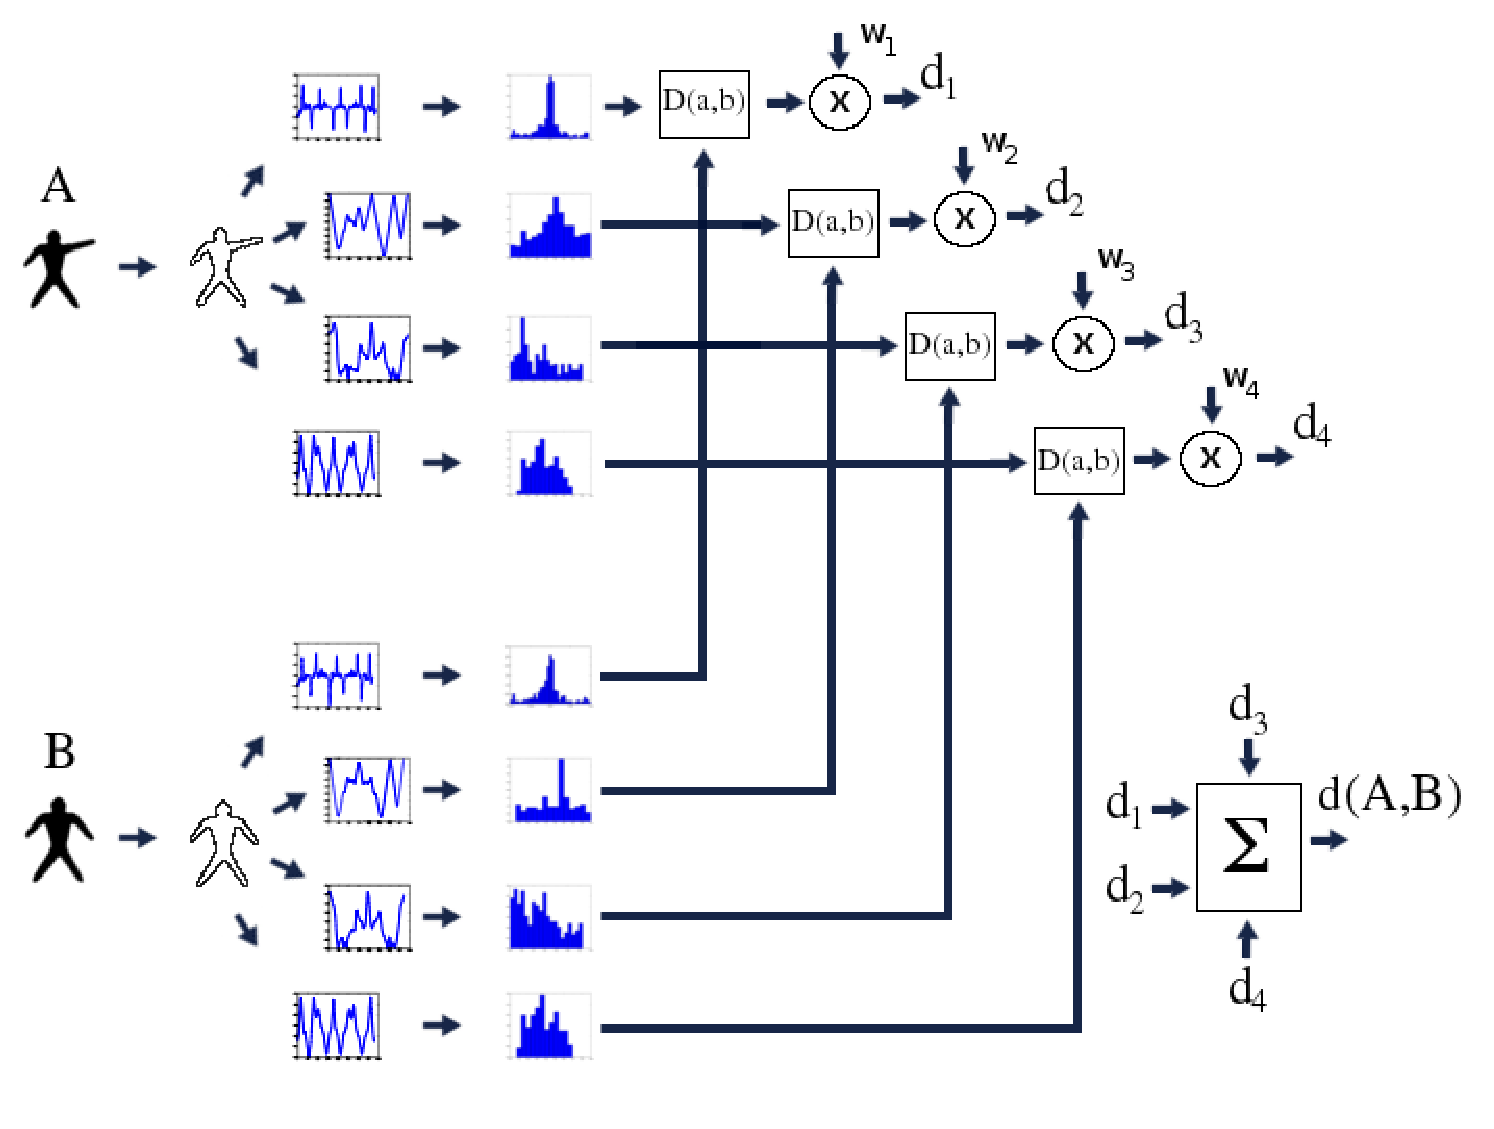
\includegraphics[width=0.85\textwidth]{figura_metodo.eps}
\end{figure}


\section{Metodologia de avaliação de desempenho}

\subsection{Experimentos CBIR}
Os experimentos de recuperação de imagens pelo conteúdo que realizamos visam avaliar o desempenho dos descritores de formas e das medidas de similaridade estudadas neste trabalho. As metodologias utilizadas nesses experimentos são as mesmas encontradas em diversos trabalhos de recuperação de formas da literatura.

São empregadas nos experimentos duas bases de imagens de formas binárias: a Kimia, de 99 formas, e a MPEG-7 CE-Shape-1 de 1400 formas. Ambas as bases estão apresentadas no Apêndice deste trabalho.

A Figura \ref{fig:metodo_cbir} ilustra a metodologia dos experimentos. Primeiramente realiza-se a extração de características das formas da base de imagens de formas binárias com o método de descrição sob avaliação. O mesmo processo de extração de características é aplicado a imagem de uma forma de consulta. Esse processo resulta numa base de dados com os vetores de características associados às formas utilizadas no experimento. 

Com a medida de similaridade avalia-se o grau de correspondência existente entre o vetor de características da forma de consulta e os vetores associados a cada uma das formas da base. Tem-se assim como resultado uma lista de imagens recuperadas em ordem decrescente de similaridade à forma de consulta. Todo esse processo é realizado repetidamente tomando-se cada forma da base de imagens como forma de consulta e recuperando-se as demais.

\begin{figure}[h!]
  \caption{\label{fig:metodo_cbir} Metodologia empregada para os experimentos de recuperação de formas pelo conteúdo.}
  \centering
  \includegraphics[width=0.55\textwidth]{Metodologia1.jpg}
\end{figure}

Na avaliação do desempenho dos experimentos duas medidas são utilizadas: o número total de acertos por posição recuperada e a medida Bull-eye.

A primeira medida consiste no número total de ocorrências de formas da mesma classe que a forma de consulta em cada posição recuperada. Um exemplo que ilustra o processo de cálculo dessa medida está apresentado na figura \ref{fig:ex_metodo_cbir}. Nesse exemplo foram realizados quatro experimentos de recuperação de formas, sendo apresentado como resultado de cada experimento as onze formas mais similares à forma de consulta. As posições aonde as formas estão destacadas em vermelho correspondem àquelas aonde a recuperação não foi correta e as demais posições, aonde não há destaque, correspondem àquelas aonde as formas foram recuperadas corretamente. Na última linha temos a medida de avaliação de desempenho. Observe que, nesse exemplo, essa é formada por onze colunas, sendo o valor em cada coluna a soma do número total de acertos dos experimentos de recuperação em cada posição correspondente.

Em alguns trabalhos de recuperação de formas pelo conteúdo, o número total de acertos por posição recuperada é calculado para a base Kimia-99 \cite{Bernier:2003}. Tendo esta base 99 formas, igualmente distribuídas em 9 classes, são realizadas 99 recuperações das 11 formas mais similares à imagem de consulta. Como resultado espera-se obter um total de 99 formas recuperadas corretamente para cada posição recuperada.

\begin{figure}[h!]
  \caption{\label{fig:ex_metodo_cbir} Exemplo ilustrando um experimento de recuperação de formas e o cálculo do número total de acertos por posição recuperada}
  \centering
  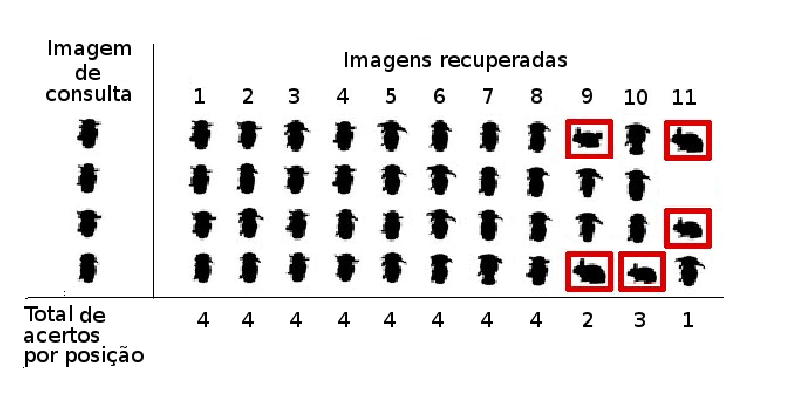
\includegraphics[width=0.75\textwidth]{ex_retrieval.eps}
\end{figure}

A medida Bull-eye também é utilizada na literatura para a comparação de diferentes métodos de recuperação de formas. Essa medida é calculada para a base MPEG-7 CE-Shape-1 da seguinte maneira: tomando-se cada forma dessa base de imagens como elemento de consulta, contabiliza-se o número de recuperações pertencentes a mesma classe da forma de consulta dentre as 40 primeiras posições recuperadas. Como resultado calcula-se a percentagem da quantidade máxima de recuperações corretas possíveis de se alcançar, sendo esta última quantidade $28000 = 1400\text{ formas} \times 20\text{ recuperações corretas poro forma}$. 

\subsection{Visualizaçâo de dados}

A Figura \ref{fig:metodo_4} ilustra o método que empregamos na avaliação da capacidade discriminativa dos descritores de formas através das técnicas de visualização dos dados apresentadas.

\begin{figure}[h!]
  \caption{\label{fig:metodo_4} Método de avaliação de descritores multiescala do contorno de formas. (a) Base de imagens. (b) Extração de características. (c) Descritores de formas. (d) Análise de similaridade a partir da matriz-U. (e) Avaliação de agrupamentos a partir da medida silhouette.}
  \centering
  \includegraphics[width=0.75\textwidth]{metodo_v4.png}
\end{figure}

O primeiro passo consiste em realizar a extração de características num conjunto de formas binárias rotuladas (Figura \ref{fig:metodo_4}a e Figura \ref{fig:metodo_4}b) com o método de descrição sob análise. Como resultado temos um conjunto de descritores, ou vetores de características, das referidas formas (Figura \ref{fig:metodo_4}c). 

A avaliação de qualidade dos descritores se dá qualitativamente e quantitativamente. Na avaliação qualitativa (Figura \ref{fig:metodo_4}d) utilizamos a rede auto-organizável de Kohonen para obtenção da matriz de distâncias unificada, ou matriz-U. Essa última é empregada como ferramenta de visualização dos dados, o que possibilita identificar como o método de descrição sob avaliação agrupa as formas. 

Na avaliação quantitativa (Figura \ref{fig:metodo_4}e) utilizamos os rótulos e os vetores de características das formas para calculamos a medida de avaliação de agrupamentos \emph{Silhouette} \cite{Rousseeuw:1987}. Valores médios dessa medida, por classe de formas, indica a habilidade dos descritores em discriminar formas que pertençam a classes distintas e de agrupar formas que pertençam a uma mesma classe.
\begin{comment}

\section{Fusão de características}

Conforme ilustra a Figura \ref{fig:features1} contruímos três bases de dados de vetores de características multiescala a partir das formas da base da Figura \ref{fig:db1}. A aplicação da técnica PCA às características multiescala possibilita obter como saída vetores de componentes descorrelacionadas e de máxima variância (citar). 

\begin{figure}[h!]
  \caption{\label{fig:features1} Metodologia que emprega a técnicas \emph{PCA} para obtenção de um descritor híbrido através da fusão de descritores multiescala.}
  \centering
  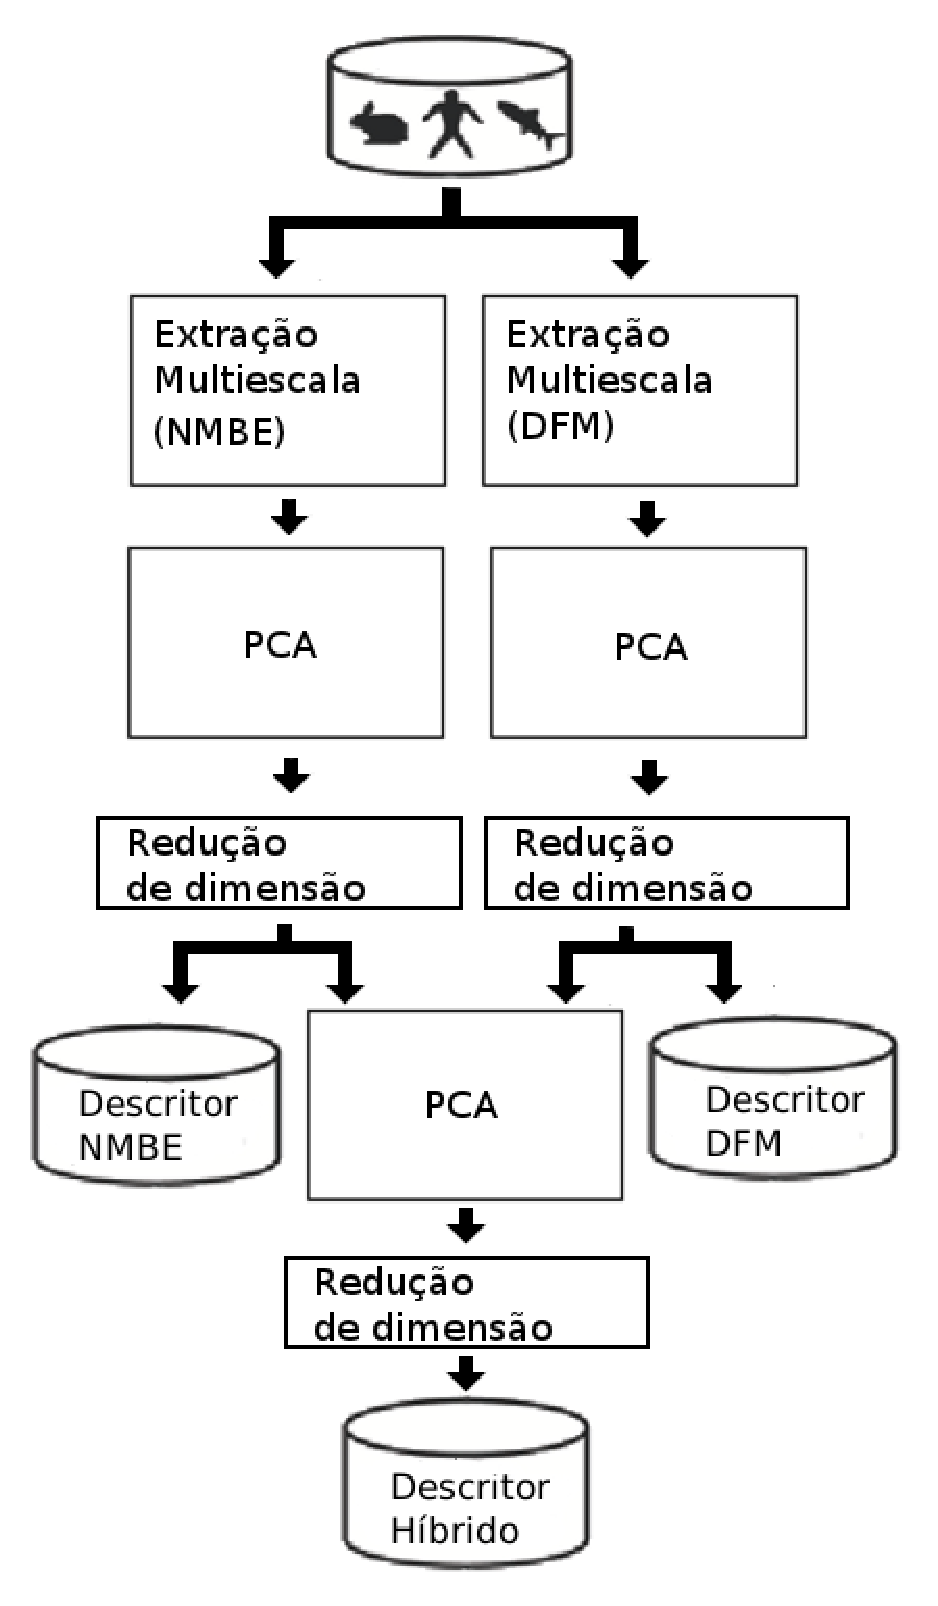
\includegraphics[width=0.45\textwidth]{features1.eps}
\end{figure}

\begin{figure}[h!]
  \caption{\label{fig:acuracia} Acurácia média por classe aferida nos experimentos de recuperação de formas pelo conteúdo, com a base Kimia-99, para os descritores (a) Dimensão fractal multiescala; (b) Energia de dobramento multiescala.}
  \centering
  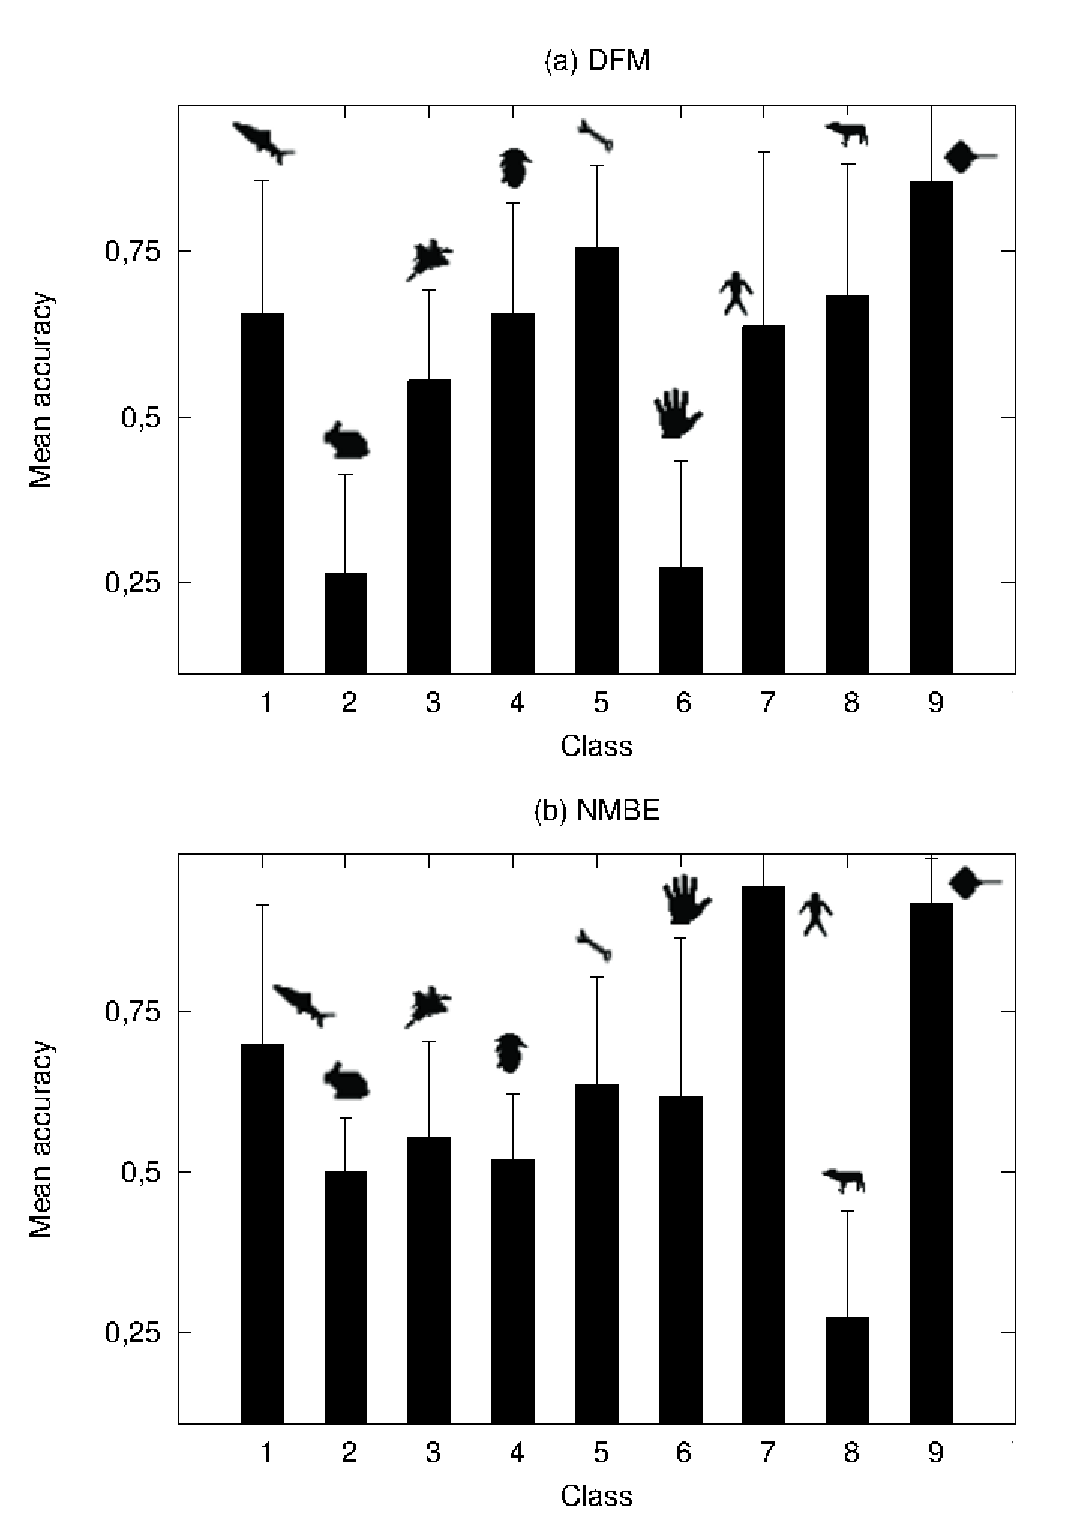
\includegraphics[width=0.75\textwidth]{resultado_acuracia.eps}
\end{figure}

\end{comment}

\color{black}
\begin{comment}
\section{Bases de imagens}
\end{comment}
\begin{comment}
\begin{figure}
\centering
\caption{\label{Met:1}Metodologia 1}
\includegraphics[width=0.5\textwidth]{Metodologia1.eps}
\end{figure}

\begin{figure}
\centering
\caption{\label{Met:2}Metodologia 2}
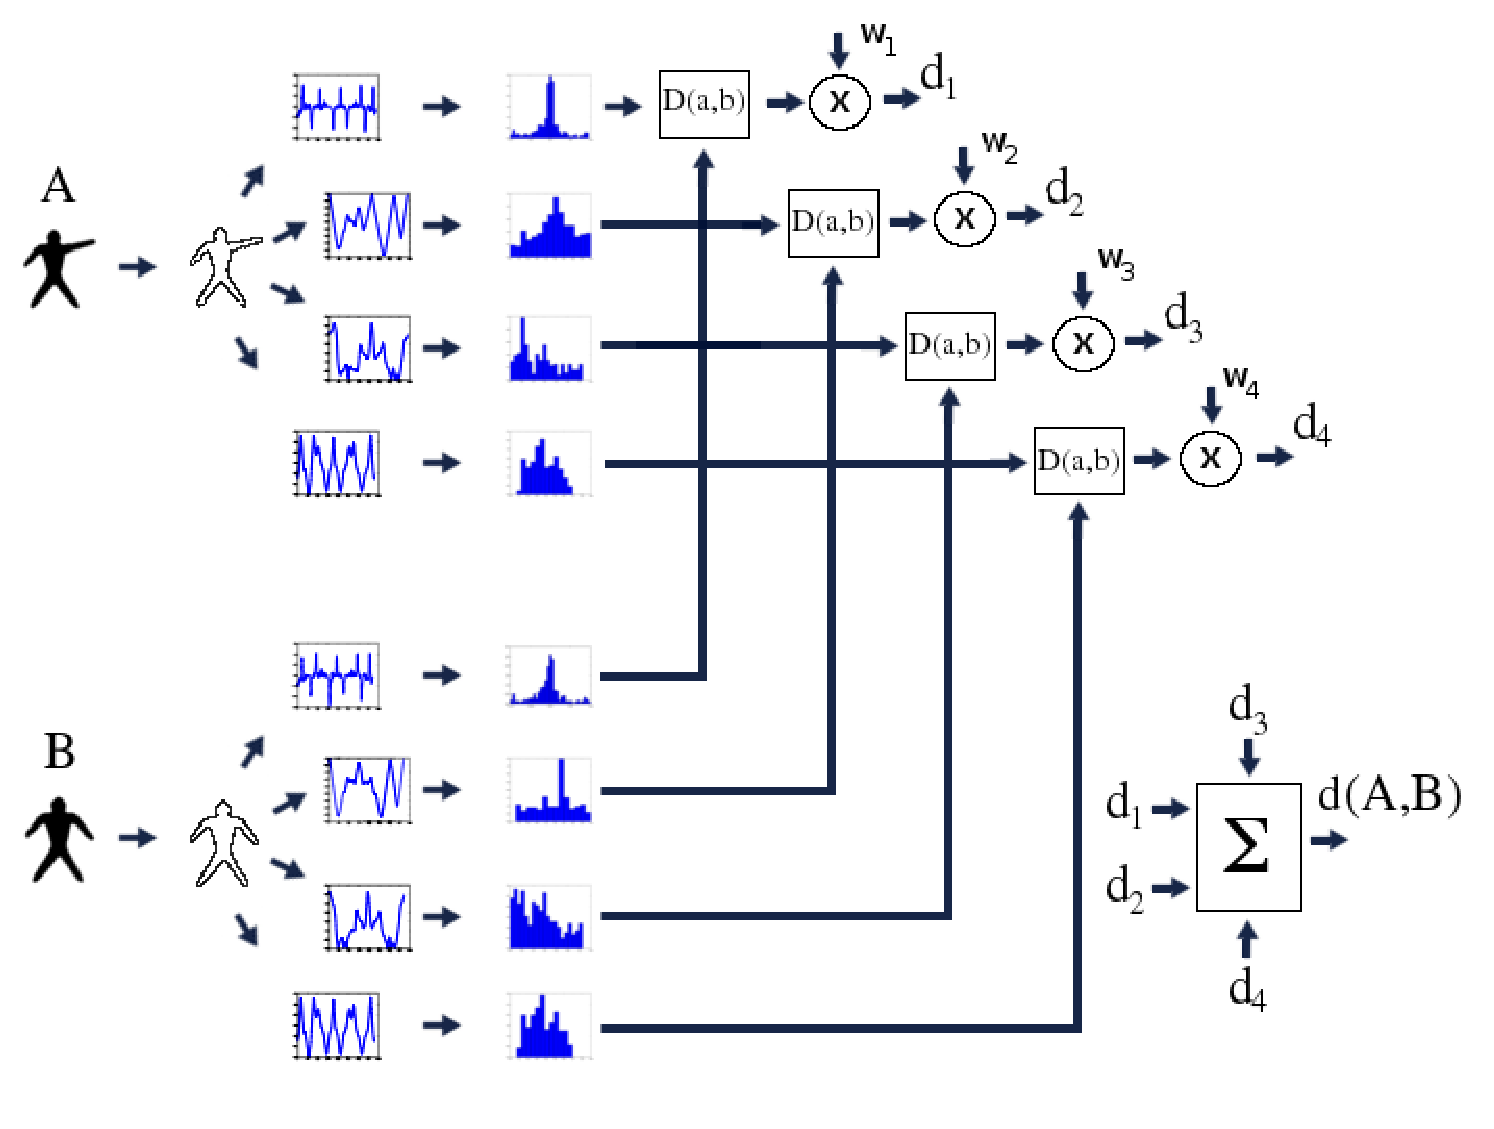
\includegraphics[width=\textwidth]{figura_metodo.eps}
\end{figure}
\end{comment}
\chapter{Metodologia}
\label{chap:MatMet}

O Capítulo \ref{chap:FUNDA} apresentou alguns dos métodos encontrados na literatura para a representação computacional de formas a partir do contorno.  Em muitos casos, esses métodos apresentam parâmetros que requerem ajustes dependentes da natureza da aplicação, ou seja,  das características da base de imagens e o propósito ao qual o sistema de reconhecimento se destina. A energia de dobramento multiescala, por exemplo, requer o ajuste do número e dos valores das escalas utilizadas na representação das formas. 

Esse capítulo apresenta um método robusto e versátil para o ajuste desses parâmetros para customizar descritores multiescala à base de imagens de formas, para fins de melhoria do desempenho em classificação supervisionada e não supervisionada. 

\section{Base de imagens}
Temos na Figura \ref{fig:leaves} exemplares de folhas extraídas da base de imagens Flavia \cite{}.

\begin{figure}[!ht]
\caption{\label{fig:leaves} Trinta e duas amostras extraídas da base Flavia, que contém $1907$ imagens de folhas de $32$ espécies diferentes. Cada amostra corresponde a uma espécie.}
\centering
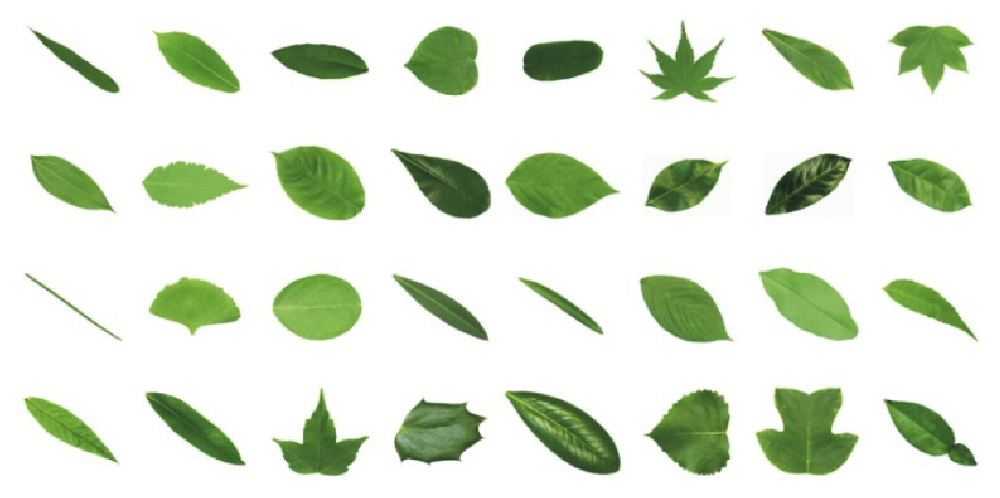
\includegraphics[width= \textwidth]{folhas.eps}
\end{figure}

\section{Extração de atributos}

\subsection{Energia de dobramento multiescala\label{subsec:BE}}

\citeonline{Young:1974} propuseram a energia de dobramento como uma medida de complexidade para análise de formas biológicas. Conceitualmente, esta é definida como sendo a energia necessária para se modificar uma forma, através de deformações, ao seu estado de menor energia, ou seja, um círculo do mesmo perímetro da forma deformada.

A maneira mais direta de se obter a energia de dobramento de um contorno fechado é a partir de sua curvatura pela seguinte expressão:

\begin{equation}\label{eq:be}
E = \frac{1}{L}\int\limits_{l}K^2(l)dl\text{,}
\end{equation}
\noindent
sendo $L$ o perímetro do contorno e a integral calculada ao longo do comprimento de seu arco. O resultado da equação \ref{eq:be} é um escalar que representa a energia média do sinal da curvatura.

\begin{comment}
A energia de dobramento multiescala é obtida a partir da curvatura multiescala repetindo-se o cálculo da equação \ref{eq:be} para diferentes níveis de suavização do contorno. Isso resulta em um vetor de características composto por escalares decorrentes da curvatura multiescala para cada uma das escalas empregadas na suavização do contorno e cálculo da curvatura. 
\end{comment}

A energia de dobramento multiescala foi introduzida por \citeonline{Costa:1997} para a análise de formas de neurônios. Nesta tese investigamos sua utilização como um descritor de propósito geral em recuperação de formas pelo conteúdo. Para um contorno discreto, com $N$ pontos, representado na forma complexa $z[n] = x[n]+jy[n] \text{,} \quad n \quad \epsilon \quad [0, \quad 1, \quad \ldots \quad , \quad N-1]$, a energia de dobramento é dada por: 

\begin{equation}
E_{be} = \frac{L^{2}}{N}\sum_{n=0}^{N-1}K^{2}[n]\text{,}
\label{eq:ebe}
\end{equation}
\noindent
sendo o perímetro do contorno elevado ao quadrado ($L^2$) uma constante de normalização para que o descritor tenha invariância a escala. A curvatura discreta $K[n]$ é calculada a partir de $z[n]$ através da seguinte expressão:

\begin{equation}
K[n] = \frac{-Im(z^{'}[n](z^{''}[n])^{*})}{|z^{'}[n]|^3} \text{,}
\label{eq:kn}
\end{equation}
\noindent
aonde $z^{'}[n]$ e $z^{''}[n]$ correspondem as derivadas primeira e segunda e $z^{*}[n]$ o conjugado de $z[n]$. 

A energia de dobramento multiescala resulta da versão discreta da curvatura multiescala. Podemos calcular as derivadas primeira e segunda do contorno discreto suavizado ($z_\sigma'[n]$ e $z_\sigma''[n]$) através das propriedades da derivada da convolução ou da transformada de Fourier. No caso discreto, a transformada de Fourier de $z[n]$ é dada por:  

\begin{equation}
Z[s] = F\big\{z[n]\big\} = \sum\limits_{n=0}^{N-1}z[n].e^{\frac{-j2\pi ns}{N}} \text{,}
\end{equation}

$s = -N_{2}\: \ldots \: N-N_{2}-1\text{, }N_{2}=floor\big(\frac{N}{2}\big)$.

 A transformada inversa é dada por  

\begin{equation}
z[n] = F^{-1}\big\{Z[s]\big\} = \sum\limits_{s = -N_{2}}^{N-N_{2}-1}Z[s]e^{\frac{j2\pi n s}{N}}\text{,}
\end{equation}
 $ n = 0\: \ldots \: N-1$.
  
No domínio $s$ o contorno é suavizado multiplicando-se, elemento a elemento, $Z[s]$ pela transformada de Fourier da versão discreta do filtro passa baixas gaussiando $g_\sigma[n] = \frac{1}{\sigma\sqrt{2\pi}}e^{\frac{n^2}{2\sigma^2}}\text{, } 
n = 0 \: \ldots \: N-1$:

\begin{equation}
Z_\sigma[s] = Z[s].F\big\{g_\sigma[n]\big\}\text{,}
\end{equation}
\noindent
 sendo as referidas derivadas do contorno suavizado:
\begin{equation}
z_\sigma'[n] = F^{-1}\big\{j2\pi s Z_\sigma[s]\big\}
\end{equation} e
\begin{equation}
z_\sigma''[n] = F^{-1}\big\{-(2\pi s)^2 Z_\sigma[s]\big\}\text{.}
\end{equation}

O processo de filtragem passa-baixas diminui a energia espectral da representação complexa do contorno resultando no encolhimento do seu perímetro. Uma estratégia para compensar tal efeito é normalizar o contorno suavizado com a razão entre o perímetro do contorno não suavizado ($L$) e o seu perímetro ($L_{\sigma}$) \cite{Cesar:1996,Costa:1997}:

\begin{equation}
\breve{z}_{\sigma}[n] = \frac{L}{L_{\sigma}}z_{\sigma}[n]\text{.}
\end{equation}

Substituindo $K[n]$ por $K_{\sigma}[n]$ e $z[n]$ por $\breve{z}_{\sigma}[n]$ nas equações \ref{eq:kn} e \ref{eq:ebe}, e realizando estes cálculos para $M$ escalas distintas $(\sigma_1\text{, }\sigma_2\text{, }\text{, }\ldots\text{, }\sigma_M)$ resulta na representação multiescala da energia de dobramento:

\begin{equation}
NMBE = (\log{E_{\sigma_{1}}}\text{, }\log{E_{\sigma_{2}}}\text{, }\ldots \text{ , }\log{E_{\sigma_{M}}})\text{.}
\label{eq:nmbe}
\end{equation}

\section{Função custo e otimização}
A metodologia para escolha de parâmetros do descritor segue o esquema da Figura \ref{fig:Avaliacao}. Essa metodologia melhora a representação do descritor utilizando métodos de otimização evolutivos para minimizar uma função custo, que corresponde a mediana do erro absoluto da \textit{silhouette} dos descritores ($MAD$). O que motivou a escolha dessa função objetivo é sua robustez a \textit{outliers} \cite{Rousseeuw:1987:2}, sendo sua equação 

\begin{equation}
\label{eq:mad}
MAD = \operatorname{mediana}\big(|s_i - 1|_{i =1,\:2,\:\cdots,\:L}\big)\text{,}
\end{equation}

\begin{figure*}[ht]
\caption{\label{fig:Avaliacao}
 Proposta de uma metodologia para otimização evolucionária de um descritor multiescala de forma.} 
\centering
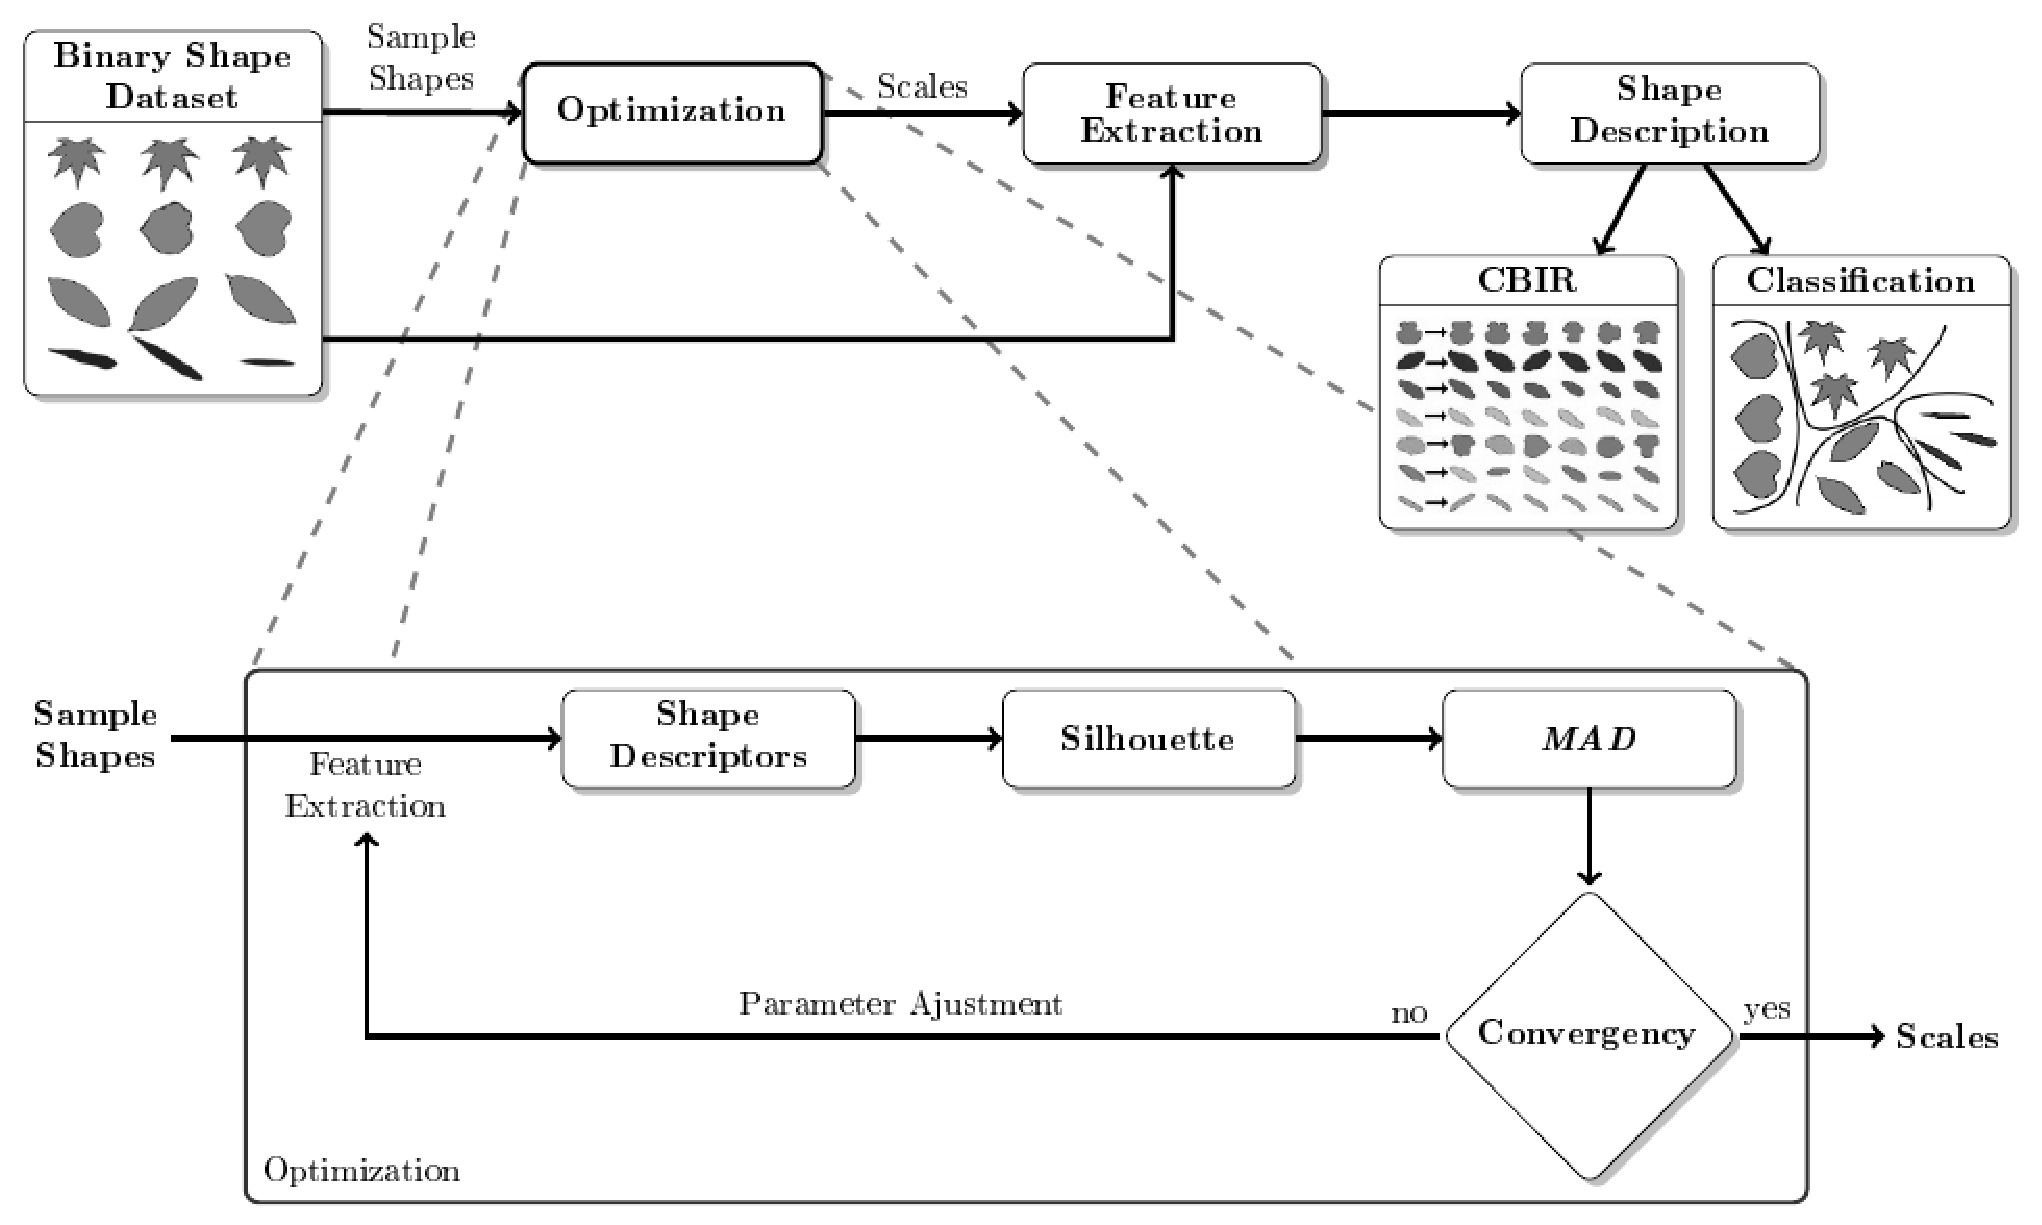
\includegraphics[width=\textwidth]{finalFlux.eps}
\end{figure*}

\noindent aonde $S = \{s_1,s_2,\cdots,s_L\}$ é o conjunto das \emph{silhouettes} calculadas para $L$ descritores de forma. Os operadores $|.|$  e {$mediana ( )$} retornam o valor absoluto e a mediana de um conjunto de valores, respectivamente.

A \textit{silhouette }\cite{Rousseeuw:1987} é uma medida de qualidade de agrupamentos que indica o grau de afinidade de uma amostra  a um agrupamento, levando em conta as distâncias médias entre classes e intra classes de um objeto $i$ atribuído a uma dada classe $A$. Logo, esta métrica é definida como 
\begin{equation}
s_i = \frac{b_i - a_i}{\max{(a_i,b_i)}} \in [-1,1],
\end{equation}

\noindent sendo $a_i$ a dissimilaridade média entre o objeto $i$ e os demais objetos pertencentes a mesma classe de $a_i$ e $b_i$ é a dissimilaridade média do objeto $i$ e a classe vizinha mais próxima de $i$, excluída sua própria classe. 

Essa métrica pode assumir valores no intervalo $[-1,1]$, sendo que valores negativos indicam que o grau de pertencimento de um objeto à classe que este fora atribuído é baixo. Já valores positivos indicam que o grau de pertencimento de um objeto à classe que este fora atribuído é alto. Um valor de silhouette próximo de zero indica que o objeto está na fronteira entre duas classes e que há, portanto, um grau de incerteza a respeito de qual classes este pertence.

Os valores da função objetivo $MAD$ assume valores no intervalo $[0,2]$. De forma análoga a silhouette, um valor igual a zero desta função indica que a estrutura dos clusters é perfeita, enquanto que valores próximos de $2$ indicam que a estrutura dos clusters é deficiente, com baixa similaridade entre os objetos de mesma classe ou alta similaridade entre os objetos de classes distintas.

%\section{Otimização}
Uma vez definida a função custo, o processo de otimização dos parâmetros descritor ajustará os mesmos ao problema em estudo. No caso da análise de formas de folhas, a otimização permite que os parâmetros, que minimizam a função objetivo ou função custo (\textit{MAD}),  incorporem nuances e detalhes do contorno das formas de folhas. O ajuste dos parâmetros ao problema em questão deverá melhorar as taxas de classificação e recuperação de formas de folhas de plantas. Vale destacar que a metodologia é versátil pois é ajustável a outras aplicações e portanto, suporta a definição de uma outra função objetivo. A Figura  \ref{fig:Avaliacao} ilustra, em detalhes, como se dá o ajuste dos parâmetros do descritor multiescala dentro da metodologia proposta, aplicada a um problema de análise de formas. Primeiramente, é amostrado na base de folhas um subconjunto das formas para, em seguida, realizar o procedimento de otimização e encontrar o melhor conjunto de parâmetros de escala  $\boldsymbol{\sigma}_{otim} = (\sigma_1,\:\sigma_2,\:\cdots,\:\sigma_k)$ do descritor NMBE que minimize a função custo da Equação \ref{eq:mad}. Então, utilizando-se as escalas encontradas realiza-se, com o descritor multiescala, a extração de características de toda a base de folhas e, em seguida, a avaliação de desempenho do mesmo.

\section{Avaliação do descritor}

O desempenho do descritor é avaliado neste trabalho qualitativamente e quantitativamente. Na avaliação qualitativa dois algoritmos de visualização de dados são utilizados: o mapa auto-organizável de Kohonen \cite{Kohonen:2001} e o \textit{escalonamento multidimensional} \cite{cox:2000}. Na avaliação quantitativa são analisadas as métricas de avaliação Precisão e Revocação, obtidas em experimentos de classificação supervisionada, a métrica \textit{Bulls-eye} \citeonline{Ling:2007:SCU:1191552.1191806}, classicamente utilizada na comparação de descritores em recuperação de formas (CBIR) e a medida de avaliação de agrupamentos silhouette \cite{Rousseeuw:1987}. 

Para fins de comparação,  as avaliações de desempenho qualitativa e quantitativa foram realizadas com as versões dos descritores otimizados com o método proposto e não otimizados, seja por escolha aleatória dos parâmetros ou por meio de ajuste apresentado em \cite{Costa:1997}.

\subsection{Visualização dos dados}

Algoritmos de visualização de dados produzem projeções bidimensionais das descrições das formas da base de folhas, provendo uma representação gráfica que possibilita a análise da qualidade dos agrupamentos. Assim, consegue-se inferir o quão eficaz o descritor é em organizar espacialmente as formas. Os métodos de visualização empregados neste trabalho são o mapa auto-organizável de Kohonen \cite{Kohonen:2001} e o \textit{escalonamento multidimensional (MDS)} \cite{cox:2000}.

As projeções \textit{MDS} da Figura \ref{fig:optimization_result} ilustram como os agrupamentos evoluem à medida que o algoritmo DE busca os parâmetros otimizados do descritor (NMBE). As amostras de formas exibidas pertencem à base Kimia-99 \cite{Sebastian:2004}, a qual contém $99$ imagens. Neste trabalho aplicamos técnicas de aprendizagem (\textit{manifold learning}) para produzir as projeções MDS do descritor NMBE otimizado utilizando o algoritmo DE.  A Figura \ref{fig:optimization_result} demonstra que à medida que os valores de MAD decrescem, as distâncias entre as classes aumentam e consequentemente os agrupamentos das classes se tornam mais evidentes. Nesta imagem, quando o método de otimização converge, ou seja MAD alcança o menor valor,   os únicos agrupamentos que não estão bem separados são aqueles relacionados às formas de animais quadrúpedes e de mãos. 

\begin{figure}[t]
\caption{\label{fig:optimization_result} Projeções do escalonamento multidimensional das formas da base Kimia-99 \citeonline{Sebastian:2004}. As imagens mostram como os agrupamentos evoluem ao longo do processo de otimização (DE), assim como os valores de MAD e $R^2$.}
\centering
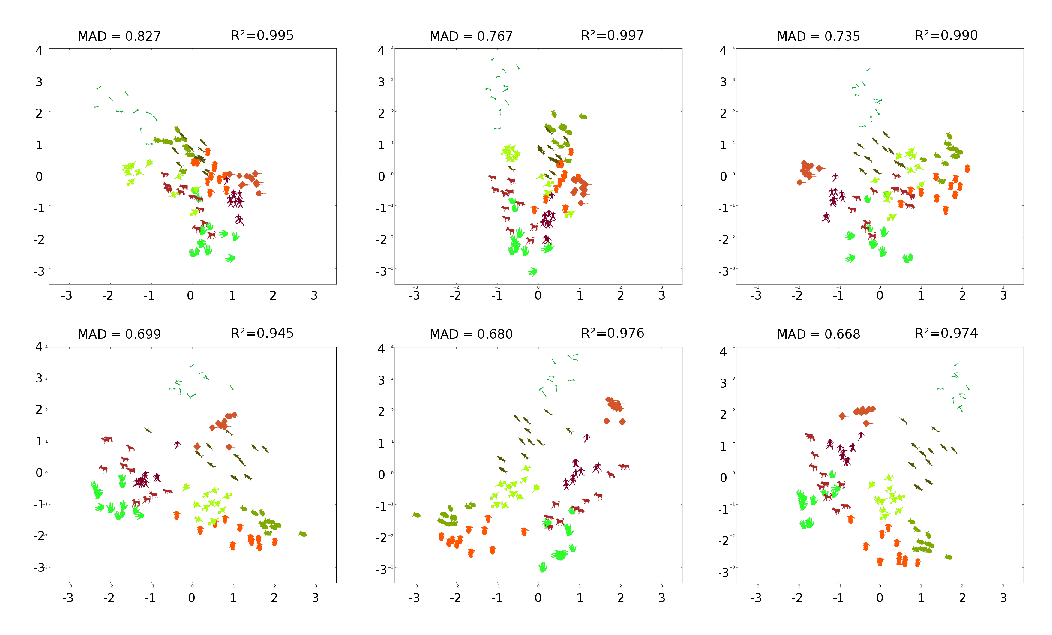
\includegraphics[width = \textwidth]{fig4.eps}
\end{figure}

\begin{figure}[!ht]
\caption{\label{fig:projkimia99} Matrizes-U para as formas da base MPEG7 CE-Shape-1.}
\centering
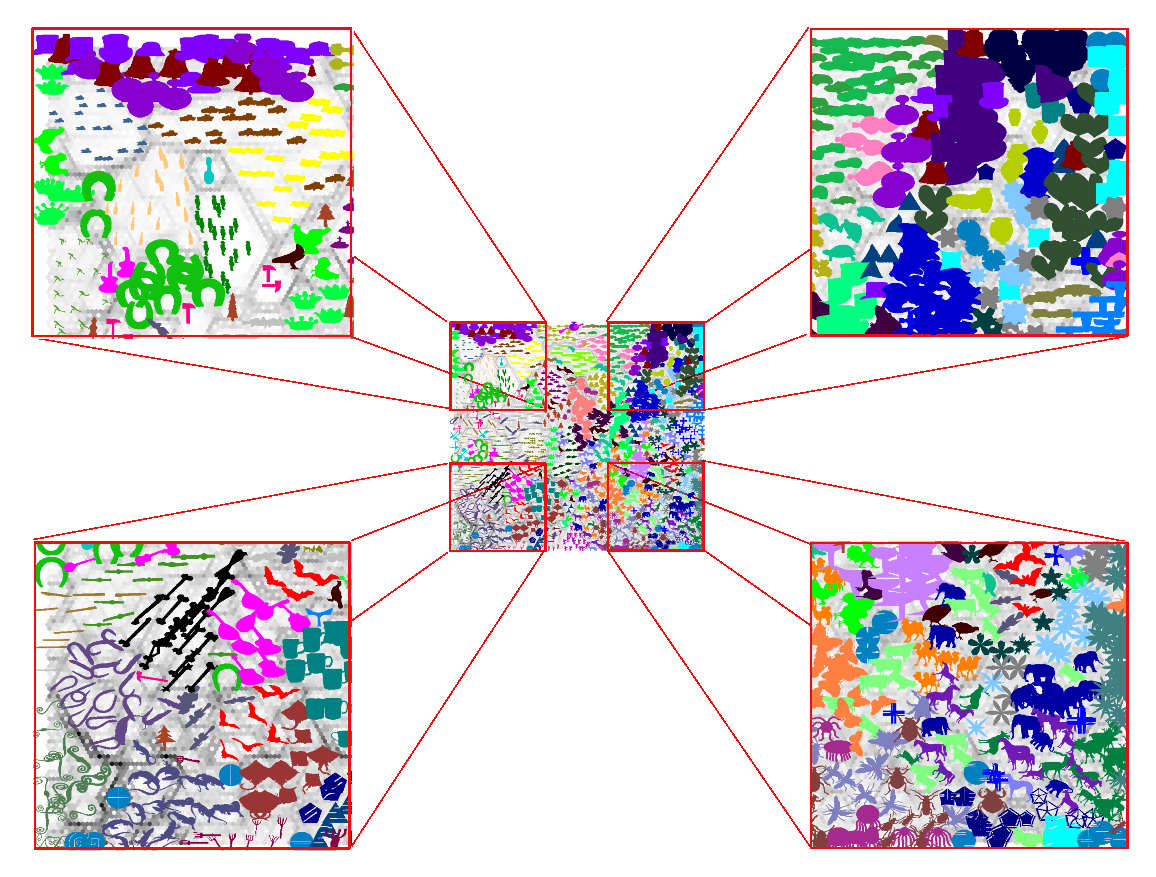
\includegraphics[width=\textwidth]{fig3.eps}
\end{figure}

\subsection{Recuperação de formas (CBIR)}

Foram realizados experimentos de recuperação de imagens pelo conteúdo visando avaliar o desempenho dos descritores de formas e das medidas de similaridade estudadas neste trabalho. As metodologias utilizadas nesses experimentos são as mesmas encontradas em diversos trabalhos de recuperação de formas da literatura.

Foram realizados experimentos em duas bases de imagens de formas binárias: a Kimia, de 99 formas, e a MPEG-7 CE-Shape-1 de 1400 formas. Ambas as bases estão apresentadas no Apêndice deste trabalho.

A  Figura \ref{fig:metodo_cbir} ilustra a metodologia dos experimentos de recuperação de formas.  Primeiramente realiza-se a extração de características das formas da base de imagens de formas binárias com o método de descrição sob avaliação. O mesmo processo de extração de características é aplicado a imagem de uma forma de consulta. Esse processo resulta numa base de dados com os vetores de características associados às formas utilizadas no experimento. 

Com a medida de similaridade avalia-se o grau de correspondência existente entre o vetor de características da forma de consulta e os vetores associados a cada uma das formas da base. Tem-se assim como resultado uma lista de imagens recuperadas em ordem decrescente de similaridade à forma de consulta. Todo esse processo é realizado repetidamente tomando-se cada forma da base de imagens como forma de consulta e recuperando-se as demais.

\begin{figure}[h!]
  \caption{\label{fig:metodo_cbir} Metodologia empregada para os experimentos de recuperação de formas pelo conteúdo.}
  \centering
  \includegraphics[width=0.55\textwidth]{Metodologia1.jpg}
\end{figure}

Na avaliação do desempenho dos experimentos duas medidas são utilizadas: o número total de acertos por posição recuperada e a medida bull-eyes.

A primeira medida consiste no número total de ocorrências de formas da mesma classe que a forma de consulta em cada posição recuperada.  Em diversos trabalhos de recuperação de formas pelo conteúdo o número total de acertos por posição recuperada é calculado para a base Kimia-99 \cite{Bernier:2003}. Tendo esta base 99 formas, igualmente distribuídas em 9 classes, são realizadas 99 recuperações das 11 formas mais similares à imagem de consulta. Como resultado espera-se obter um total de 99 formas recuperadas corretamente para cada posição recuperada.

A medida Bulls-eye também é utilizada na literatura para a comparação de diferentes métodos de recuperação de formas. Essa medida é calculada para a base MPEG-7 CE-Shape-1 da seguinte maneira: tomando-se cada forma dessa base de imagens como elemento de consulta, contabiliza-se o número de recuperações pertencentes a mesma classe da forma de consulta dentre as $40$ primeiras posições recuperadas. Como resultado calcula-se a percentagem da quantidade máxima de recuperações corretas possíveis de se alcançar, sendo esta última quantidade $28000 = 1400\text{ formas} \times 20\text{ recuperações corretas poro forma}$. 

\subsection{Classificação supervisionada}

\begin{figure*}[]
\caption{\label{fig:Classific}
Metodologia de classificação para avaliação de desempenho do descritor otimizado pelo método proposto exibido na Figura.  \ref{fig:Avaliacao}} 
\centering
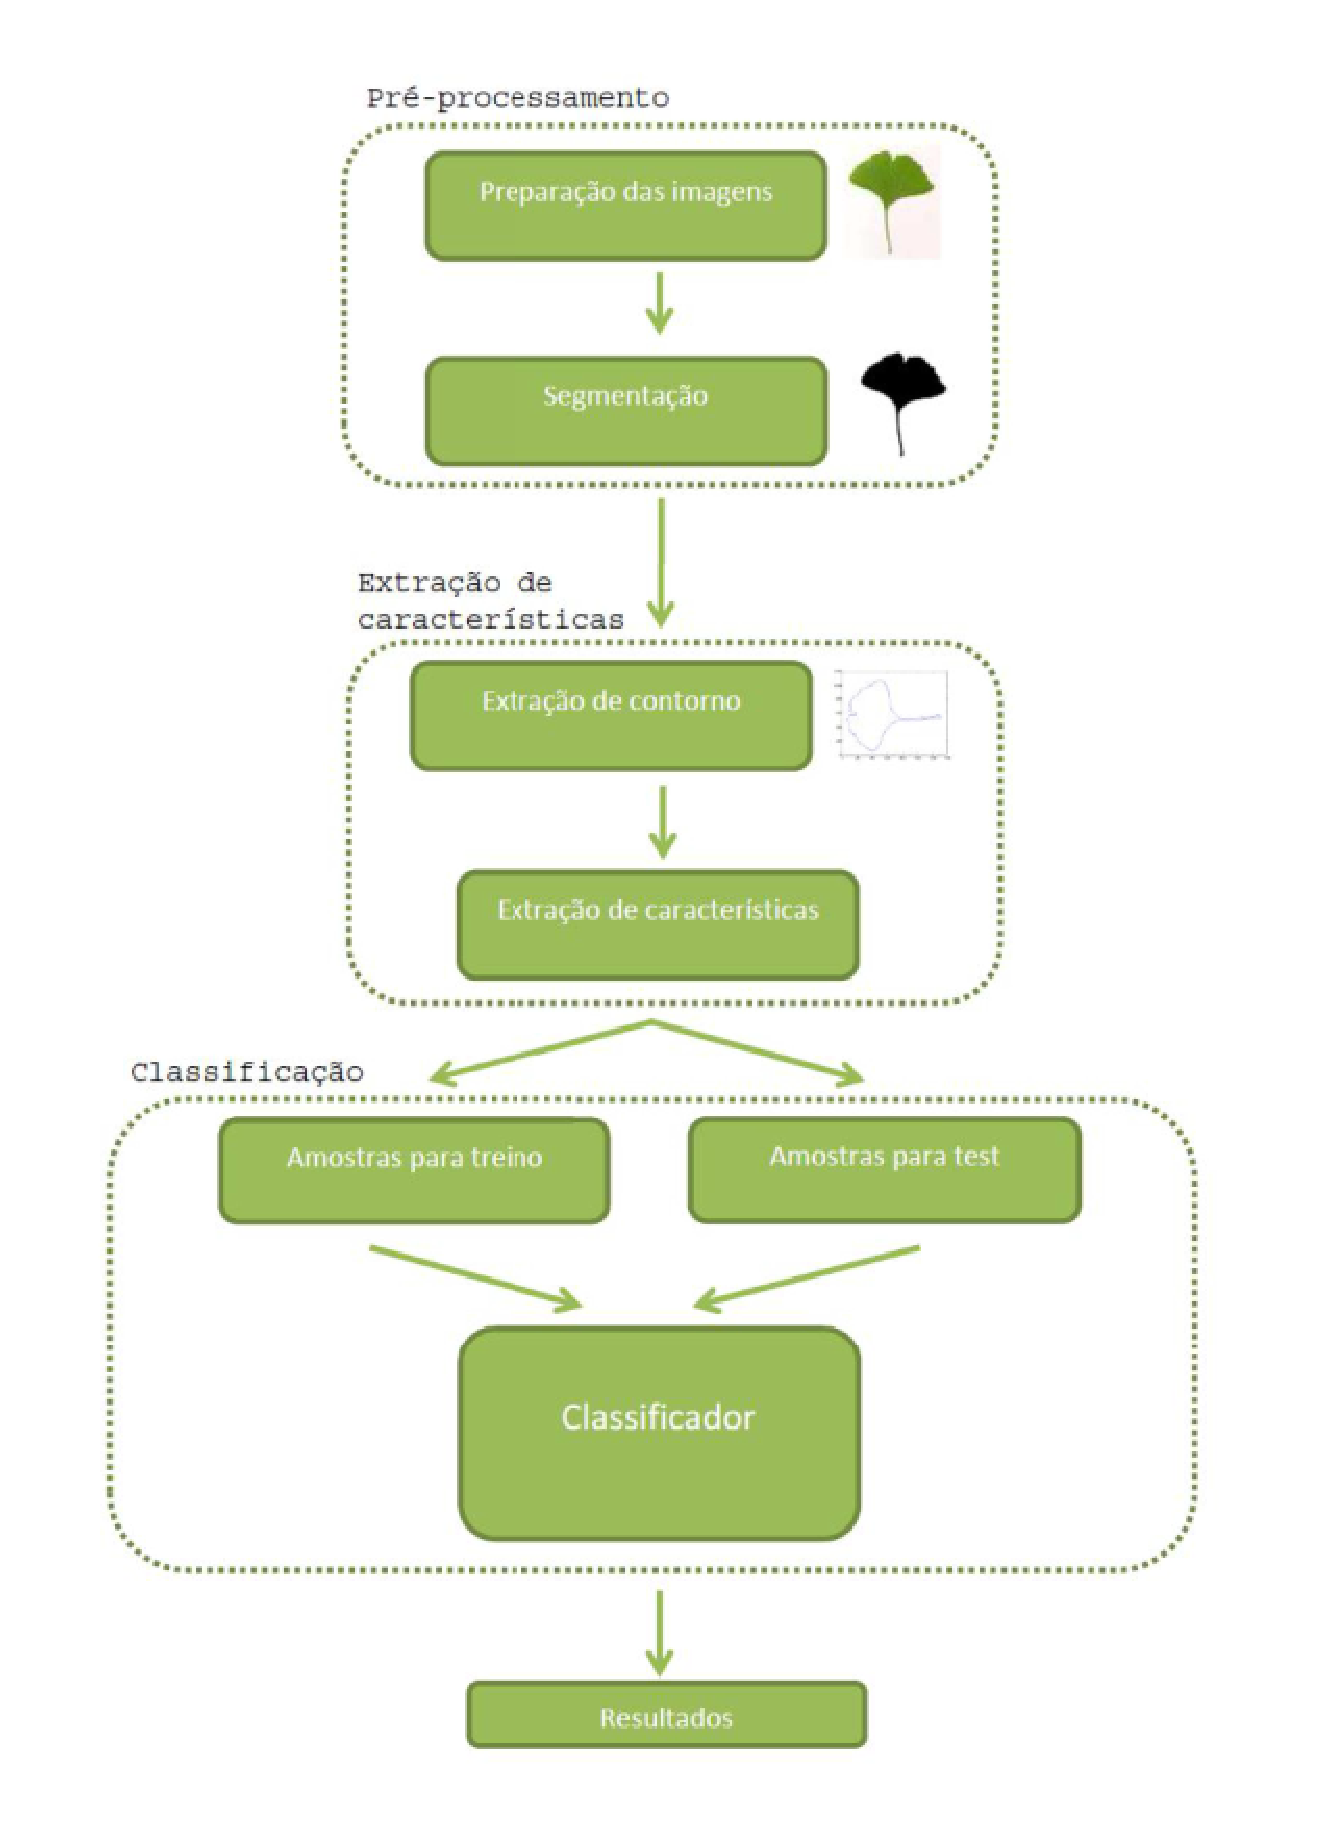
\includegraphics[width=0.7\textwidth]{fig_metodo_classifica_folhas.eps}
\end{figure*}

O procedimento adotado para avaliar o desempenho do descritor multiescala em classificação supervisionada está ilustrado na Figura \ref{fig:Classific}. A etapa de pré-processamento consiste na segmentação das imagens das formas. Essa etapa só se aplica para a base de folhas Flavia, aonde um método  de segmentação por limiar \cite{Gonzalez:2006} foi empregado. Para as formas das bases MPEG7-CE e Kimia-99, esta etapa não é necessária, pois as formas destas bases estão disponíveis já binarizadas.

Após a extração de características das formas, os descritores obtidos (vetores de características) são divididos em grupos de amostras de teste/treino pelo método de validação cruzada K-Fold (K = 10) \cite{Webb:2002}. Então, os descritores são transformados pelo discriminante linear de Fisher \cite{Webb:2002}, para melhorar a separação inter classes e a coesão intra classe, e em seguida, pela análise das componentes principais (PCA) para descorrelacioná-los. Cabe aqui salientar que as matrizes dessas transformações são obtidas apenas considerando as amostras de treino.

A etapa de classificação utiliza os classificadores Naive Bayes (NB) \cite{Fukunaga:1990}, \emph{K}-vizinhos próximos (Knn, $K = 5$) \cite{Fukunaga:1990,Webb:2002},  o discriminante linear de Fisher (LDA) \cite{Webb:2002} e o discriminante quadrático (QDA) \cite{Fukunaga:1990}. Para cada classificador foram realizadas $100$ execuções da validação cruzada, tendo como resultado os valores médios e os desvios da precisão e revocação obtidos nesses experimentos.  As medidas clássicas de precisão e revocação são empregadas na avaliação do desempenho de descritores em experimentos de classificação supervisionada.


\subsection{Avaliação quantitativa de agrupamentos}

A \textit{silhouette} média por classe avalia tanto a coesão como a separação das classes através da distância entre os vetores de características.




%A avaliação de similaridade entre formas a partir de medidas de divergência requer que as informações das assinaturas, abordadas na Seção \ref{sec:Assinatura} do Capítulo \ref{chap:contour}, sejam tratadas como variáveis aleatórias e que suas distribuições de probabilidade sejam estimadas. 

%A  Figura \ref{fig:metodo_distancia} ilustra como divergentes podem ser aplicados na avaliação da similaridade entre duas formas A e B. No método em questão, as distribuições de probabilidade de quatro assinaturas distintas dos contornos das formas são estimadas, através de histogramas, para em seguida se calcular as medidas de divergência. Uma medida de similaridade é então obtida  a partir da média ponderada das medidas de divergência.

\begin{comment}
\subsection{Visualização de dados}

A Figura \ref{fig:metodo_4} ilustra o método que empregamos na avaliação da capacidade discriminativa dos descritores de formas através das técnicas de visualização dos dados apresentadas.

\begin{figure}[h!]
  \caption{\label{fig:metodo_4} Método de avaliação de descritores multiescala do contorno de formas. (a) Base de imagens. (b) Extração de características. (c) Descritores de formas. (d) Análise de similaridade a partir da matriz-U. (e) Avaliação de agrupamentos a partir da medida silhouette.}
  \centering
  \includegraphics[width=\textwidth]{metodo_v4.png}
\end{figure}

O primeiro passo consiste em realizar a extração de características num conjunto de formas binárias rotuladas (Figura \ref{fig:metodo_4}a e Figura \ref{fig:metodo_4}b) com o método de descrição sob análise. Como resultado temos um conjunto de descritores, ou vetores de características, das referidas formas (Figura \ref{fig:metodo_4}c). 

A avaliação de qualidade dos descritores se dá qualitativamente e quantitativamente. Na avaliação qualitativa (Figura \ref{fig:metodo_4}d) utilizamos a rede auto-organizável de Kohonen para obtenção da matriz de distâncias unificada, ou matriz-U. Essa última é empregada como ferramenta de visualização dos dados, o que possibilita identificar como o método de descrição sob avaliação agrupa as formas. 

Na avaliação quantitativa (Figura \ref{fig:metodo_4}e) utilizamos os rótulos e os vetores de características das formas para calculamos a medida de avaliação de agrupamentos \emph{Silhouette} \cite{Rousseeuw:1987}. Valores médios dessa medida, por classe de formas, indica a habilidade dos descritores em discriminar formas que pertençam a classes distintas e de agrupar formas que pertençam a uma mesma classe.
\end{comment}

\begin{comment}
Although the curvature signal is a sensitive signature to local features of the shape contour, such as concavity and spatial location of salient points, its low noise immunity limits it for shape description application. Thus, it is recommended to smooth  the contour before calculating the curvature signal in order to yield a more robust representation, albeit losing information \citep{Cesar:1996}. A usual smoothing strategy is the discrete convolution of $z[n]$ with a Gaussian kernel, as follows

\begin{equation}
z_{\sigma}[n] = \sum_{i=1}^{N}z[i]g_{\sigma}[n-i],
\label{eq:zsigma}
\end{equation}

\noindent where $g_{\sigma}[n]$ is a Gaussian kernel filter and
$\sigma$ stands for the scale parameter for smoothing control. The Gaussian filter $g_{\sigma}[n]$ is given by\\ 

\begin{equation}
g_{\sigma}[n] = \frac{1}{\sigma\sqrt{2\pi}}e^{-n^{2}/2\sigma^{2}}. 
\end{equation}


It is well-known that this filtering process modifies the amplitude of the respective spectral representation of the contour in such a way that the contour tends to shrink as the kernel scale parameter decreases \citep{Cesar:1996,Costa:1997}. One strategy to avoid such effect is to normalize the smoothed contour as

\begin{equation}
\breve{z}_{\sigma}[n] = \frac{P}{P_{\sigma}}z_{\sigma}[n],
\end{equation}

\noindent where $P$ and $P_{\sigma}$ are the perimeters of the non-smoothed and smoothed contours, respectively.

By replacing $k[n]$ by $k_{\sigma}[n]$ and $z[n]$ by $\breve{z}_{\sigma} [n]$ in equations \ref{eq:ebe} and \ref{eq:kn}, and calculating these equations for $M$ different smoothing scale factors  $\sigma = (\sigma_{1}\text{, }\sigma_{2}\text{, }\ldots\text{ , }\sigma_{M})$, we obtain a multiscale representation of the bending energy given by:

\begin{equation}
NMBE = (\log{E_{\sigma_{1}}}\text{, }\log{E_{\sigma_{2}}}\text{, }\ldots \text{ , }\log{E_{\sigma_{M}}}).
\label{eq:nmbe}
\end{equation}
\end{comment}


%Os descritores entropia multiescala, apresentado no Capítulo \ref{chap:FUNDA}, e a energia de dobramento multiescala requerem o ajuste dos seguintes parâmetros: o número e os valores dos fatores de escala utilizados na representação das formas. Esse capítulo apresenta um método robusto e versátil para o ajuste desses parâmetros para customizar esses descritores em aplicações de classificação supervisionada e não supervisionada.   

\chapter{Metodologia}
\label{chap:MatMet}

O Capítulo \ref{chap:FUNDA} apresentou alguns dos métodos encontrados na literatura para a representação computacional de formas a partir do contorno.  Em muitos casos, esses métodos apresentam parâmetros que requerem ajustes dependentes da natureza da aplicação, ou seja,  das características da base de imagens e o propósito ao qual o sistema de reconhecimento se destina. A energia de dobramento multiescala, por exemplo, requer o ajuste do número e dos valores das escalas utilizadas na representação das formas. 

Esse capítulo trata do método proposto neste trabalho, que customizar descritores multiescala à base de imagens de formas melhorando o desempenho em classificação supervisionada e não supervisionada. Inicialmente é apresentando, em linhas gerais, o método em questão para em seguida detalhar cada uma das etapas envolvidas tanto no processo de customização dos descritores como na avaliação dos resultados. 

\section{Customização dos descritores\label{sec:met}}
O objetivo do método proposto para customização de descritores, cujo esquema é apresentado na Figura \ref{fig:Avaliacao}, é melhorar a representação do descritor de formas ajustando seus parâmetros através de algoritmos de otimização evolutivos. Foi utilizada como função objetivo na otimização o \ac{MAD} da métrica de avaliação de agrupamentos \textit{silhouette} \cite{Rousseeuw:1987}. O que motivou a escolha dessa função objetivo é sua robustez a \textit{outliers} \cite{Rousseeuw:1987:2}, sendo sua equação definida por

\begin{equation}
\label{eq:mad}
MAD = \operatorname{mediana}\big(|s_i - 1|_{i =1,\:2,\:\cdots,\:L}\big)\text{,}
\end{equation}

\begin{figure*}[ht]
\caption{\label{fig:Avaliacao}
 Proposta de uma metodologia para otimização evolucionária de um descritor multiescala de forma.} 
\centering
\includegraphics[width=\textwidth]{finalFlux1.jpg}
\end{figure*}

\noindent sendo $S = \{s_1,s_2,\cdots,s_L\}$ é o conjunto das \emph{silhouettes} calculadas para $L$ descritores de forma. Os operadores $|.|$  e {$mediana ( )$} retornam o valor absoluto e a mediana de um conjunto de valores, respectivamente.

A \textit{silhouette }\cite{Rousseeuw:1987} é uma medida de qualidade de agrupamentos que indica o grau de afinidade de uma amostra  a um agrupamento, considerando as distâncias médias entre classes e intra classes de um objeto $i$ atribuído a uma dada classe $A$. Logo, esta métrica é definida como 
\begin{equation}
s_i = \frac{b_i - a_i}{\max{(a_i,b_i)}} \in [-1,1],
\end{equation}

\noindent sendo $a_i$ a dissimilaridade média entre o objeto $i$ e os demais objetos pertencentes a mesma classe de $a_i$ e $b_i$ é a dissimilaridade média do objeto $i$ e a classe vizinha mais próxima de $i$, excluída sua própria classe. 

Essa métrica pode assumir valores no intervalo $[-1,1]$, sendo que valores negativos indicam que o grau de afinidade de um objeto à classe que este fora atribuído é baixo. Já valores positivos indicam alta afinidade de um objeto à classe que este fora atribuído. Um valor de \textit{silhouette} próximo de zero indica que o objeto está na fronteira entre duas classes e que há, portanto, um grau de incerteza a respeito de qual classes este pertence.

A função objetivo \ac{MAD} assume valores no intervalo $[0,2]$. De forma análoga à \textit{silhouette}, um valor igual a zero indica que a estrutura dos agrupamentos é perfeita, enquanto que valores próximos de $2$ indicam que a estrutura dos agrupamentos é deficiente, com baixa similaridade entre os objetos de mesma classe ou alta similaridade entre os objetos de classes distintas.

%\section{Otimização}
Uma vez definida a função custo, o processo de otimização dos parâmetros do descritor visa ajustá-lo ao problema em estudo. No caso da análise de formas de folhas, a otimização permite que os parâmetros, que minimizam a função objetivo ou função custo (\ac{MAD}), incorporem nuances e detalhes do contorno das formas de folhas. Assim, tal ajuste reflete em melhoria na acurácia da classificação e recuperação de formas de folhas de plantas. Vale destacar que a metodologia é versátil pois é ajustável a outras aplicações e portanto, suporta a definição de uma outra função objetivo. A Figura  \ref{fig:Avaliacao} ilustra, em detalhes, como ocorre o ajuste dos parâmetros do descritor multiescala de acordo com a metodologia proposta, aplicada a um problema de análise de formas. Primeiramente, é amostrado na base de folhas um subconjunto das formas para, em seguida, realizar o procedimento de otimização e encontrar o melhor conjunto de parâmetros de escala  $\boldsymbol{\sigma}_{otim} = (\sigma_1,\:\sigma_2,\:\cdots,\:\sigma_k)$ do descritor \ac{NMBE} que minimize a função custo da Equação \ref{eq:mad}. Então, utilizando-se as escalas encontradas realiza-se, com o descritor multiescala, a extração de características de toda a base de folhas e, em seguida, a avaliação de desempenho do mesmo.

\section{Bases de formas binárias}

Foram utilizadas nos experimentos três bases públicas de imagens de formas binárias sintéticas e uma base de folhas, cujas características estão apresentadas na Tabela \ref{tbl:bases}. Embora o formato das imagens em cada base seja diferente, estas foram todas convertidas, para fins de padronização, a um padrão comum, no caso o formato PNG. 

\begin{table}[b]
	\centering
	\caption{Características das bases de imagens utilizadas nos experimentos}
	\label{tbl:bases}
	\begin{tabular}{lcrr}
		\toprule
		Base de imagens       & Formato & Total de formas & Total de classes \\
		\midrule
		Kimia-99      & PNG & $99$   & $9$     \\
		Kimia-216     & PGM & $216$  & $12$    \\
		MPEG7-CE      & GIF & $1400$ & $70$    \\
		Flavia leaves & JPG & $1907$ & $32$\\
		\bottomrule
	\end{tabular}
\end{table}

A Figura \ref{fig:db1} apresenta todas as $99$ formas da base Kimia-99, enquanto as Figuras \ref{fig:db2} e \ref{fig:db3} ilustram algumas das formas da base Kimia-216 e MPEG7-CE, respectivamente.

\begin{figure}[h!]
	\caption{\label{fig:db1} Formas da base de imagens Kimia-99.}
	\centering
	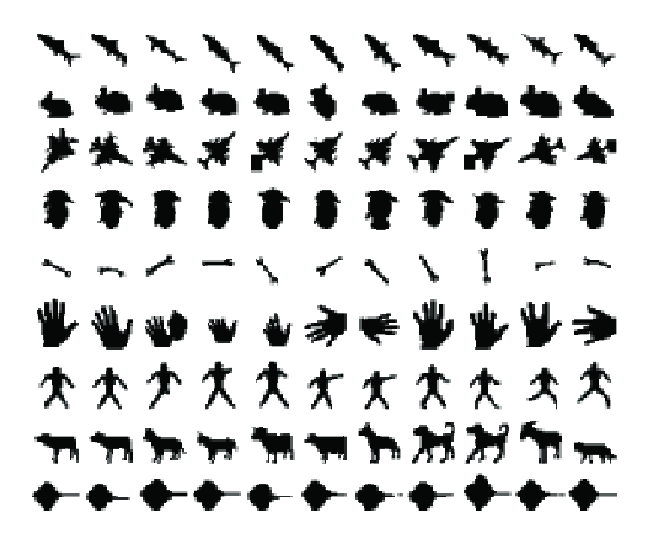
\includegraphics[width=0.5\textwidth]{db.eps}
\end{figure}

\begin{figure}[h!]
	\caption{\label{fig:db2} Amostras de formas da base de imagens Kimia-216.}
	\centering
	\includegraphics[width=0.5\textwidth]{Dataset.jpg}
\end{figure}

\begin{figure}[h!]
	\caption{\label{fig:db3} Amostras de formas da base de imagens MPEG-7.}
	\centering
	\includegraphics[width=0.5\textwidth]{mpeg7.png}
\end{figure}

Exemplares extraídos da base pública de imagens de folhas intitulada Flavia \cite{4458016} são exibidos na Figura \ref{fig:leaves}. Esta base, composta de  $1907$ imagens de folhas de $32$ espécies distintas, tem sido extensivamente utilizada em trabalhos recentes para testes de métodos de reconhecimento automático de espécies de plantas \cite{wang2015march,quteprints78723,Quadri:2015,Chaki201561}. A base Flavia é bastante desafiadora pois, além de ser desbalanceada, ou seja,  conter classes com quantidades distintas de folhas, ela ainda apresenta espécies com grande variabilidade intra classe e pequena variabilidade entre classes.

\begin{figure}[!ht]
	\caption{\label{fig:leaves} Trinta e duas amostras extraídas da base Flavia, que contém $1907$ imagens de folhas de $32$ espécies diferentes. Cada amostra corresponde a uma espécie.}
	\centering
	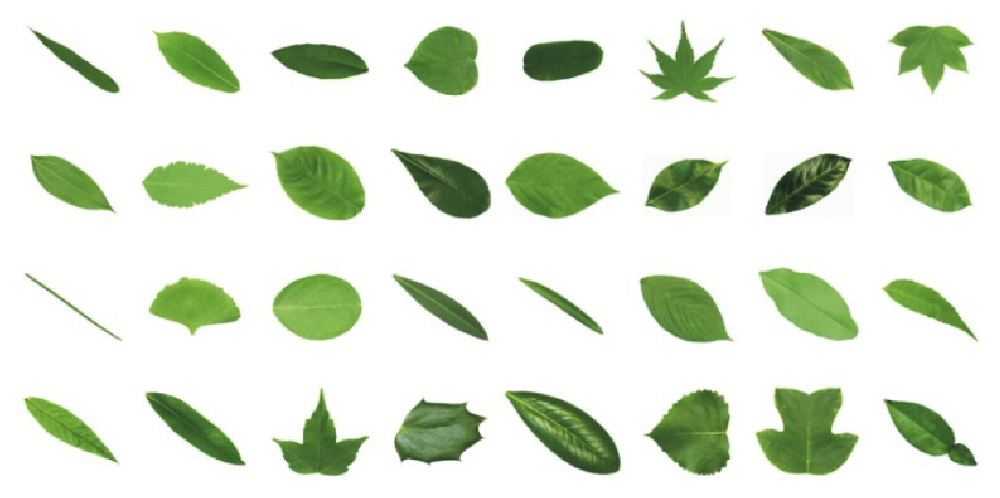
\includegraphics[width= 0.6\textwidth]{folhas.eps}
\end{figure}

\begin{comment}
\textcolor{red}{
\section{Extração de características\label{sec:EA}}
Aqui vou comentar os dois métodos de extração de características no qual vou aplicar a metodologia (IDSC e NMBE).
Vou também comentar como será feita a avaliação da 
validade do método proposto (comparação do desempenho com o ajuste de parâmetros obtido através de otimização e valores dos parâmetros sugeridos na literatura.
e por valores propostos na literatura.
}
\end{comment}
\section{Avaliação do descritor}

Nesta tese, o desempenho do descritor customizado é avaliado qualitativa e quantitativamente. Na avaliação qualitativa, dois algoritmos de visualização de dados são utilizados: o mapa auto-organizável de Kohonen \cite{Kohonen:2001} e o escalonamento multidimensional \cite{cox:2000}. Na avaliação quantitativa,  são analisadas as métricas de avaliação Precisão e Revocação \cite{Paula:2013} obtidas em experimentos de classificação supervisionada, a medida \textit{Bulls-eye} \cite{Alajlan20117,Ling:2007:SCU:1191552.1191806}, classicamente utilizada em experimentos de recuperação de formas (\ac{CBIR}) e a medida de avaliação de agrupamentos \textit{silhouette} \cite{Rousseeuw:1987}. 

Para fins de comparação,  as avaliações de desempenho qualitativa e quantitativa foram realizadas com as versões dos descritores otimizados pelo método proposto e não otimizados, seja por escolha aleatória dos parâmetros ou por meio de ajuste apresentado em \cite{Costa:1997}.

\subsection{Visualização dos dados}

Algoritmos de visualização de dados produzem projeções bidimensionais das descrições das formas da base de folhas, provendo uma representação gráfica que possibilita a análise da qualidade dos agrupamentos. Assim, consegue-se inferir o quão eficaz o descritor é em organizar espacialmente as formas.

A Figura \ref{fig:projkimia99} mostra a matriz-U \cite{Ultsch:1990} para formas da base MPEG-7 CE-Shape-1 data set \cite{855850}. Essa matriz mostra, preservando a topologia do mapa auto-organizável de Kohonen \cite{Kohonen:2001}, a relação de distância entre as estruturas mapeadas. A imagem central é o resultado do processamento de todas as imagens da base descrita pela \ac{NMBE} otimizada. As quatro imagens dos cantos são detalhes da imagem central. 

\begin{figure}[h]
\caption{\label{fig:projkimia99} Matriz-U para as formas da base MPEG7 CE-Shape-1.}
\centering
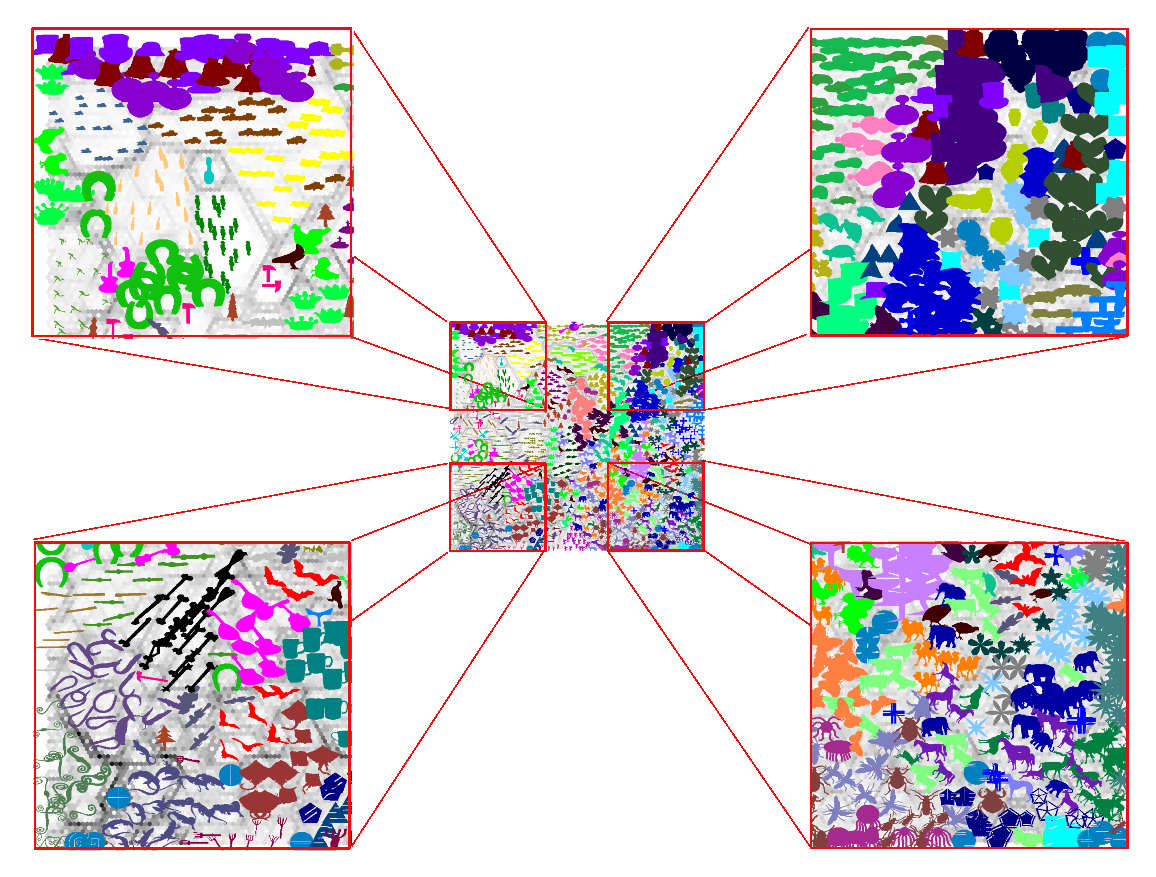
\includegraphics[width=0.8\textwidth]{fig3.eps}
\end{figure}

Essa ferramenta de visualização identifica quão bem a \ac{NMBE} descreve detalhes sutis das formas de um mesmo agrupamento e de diferentes agrupamentos. Nas imagens de detalhes se observa que as fronteiras entre os agrupamentos (cor cinza) estão evidentes e separam agrupamentos bem definidos. Nesta tese assumimos que agrupamentos bem definidos são aqueles com menor distância dentro das classes e maior distância entre classes.  

As projeções \ac{MDS} da Figura \ref{fig:optimization_result} ilustram como os agrupamentos evoluem à medida que o algoritmo \ac{DE} busca os parâmetros otimizados do descritor (\ac{NMBE}). As amostras de formas exibidas pertencem à base Kimia-99 \cite{Sebastian:2004}, a qual contém $99$ imagens. Neste trabalho, aplicamos técnicas de aprendizagem (\textit{manifold learning}) para produzir as projeções \ac{MDS} do descritor \ac{NMBE} otimizado utilizando o algoritmo \ac{DE}.  A Figura \ref{fig:optimization_result} demonstra que à medida que os valores de \ac{MAD} decrescem, as distâncias entre as classes aumentam e consequentemente os agrupamentos das classes se tornam mais evidentes. Nesta figura, quando o método de otimização converge, ou seja \ac{MAD} alcança o menor valor,   os únicos agrupamentos que não estão bem separados são aqueles relacionados às formas de animais quadrúpedes e de mãos.

\begin{figure}[h]
\caption{\label{fig:optimization_result} Projeções do escalonamento multidimensional das formas da base Kimia-99 \citeonline{Sebastian:2004}. As imagens mostram como os agrupamentos evoluem ao longo do processo de otimização (\ac{DE}), assim como os valores de \ac{MAD} e $R^2$.}
\centering
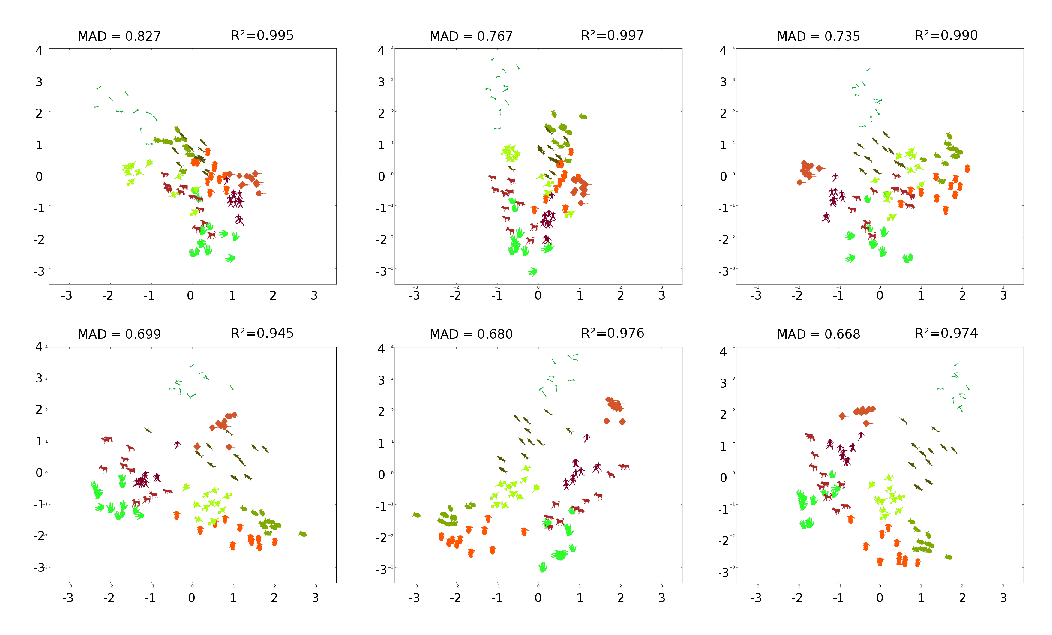
\includegraphics[width = \textwidth]{fig4.eps}
\end{figure}

\subsection{Recuperação de formas}

Visando avaliar o desempenho dos descritores de  forma, foram realizados experimentos de recuperação de imagens pelo conteúdo em duas bases de imagens de formas binárias (Kimia-99 e MPEG-7 CE-Shape-1) e uma  base de folhas (Flavia). 

A  Figura \ref{fig:metodo_cbir} ilustra a metodologia dos experimentos de recuperação de formas.  Primeiramente realiza-se a extração de características das formas da base de imagens com o método de descrição sob avaliação. Desse processo, resulta uma base de dados com os vetores de características associados às formas, que serão utilizados no experimento. 

O mesmo processo de extração de características é aplicado à imagem da forma de consulta. Essa última corresponde ao padrão de entrada ao qual as demais formas da base serão comparadas, através de uma medida de similaridade, a fim de se estabelecer o grau de correspondência existente entre as mesmas. Desta forma, tem-se como resultado a lista das imagens recuperadas na ordem decrescente da similaridade que apresentam em relação à forma de consulta. Todo esse processo é realizado tomando-se cada forma da base de imagens como forma de consulta para realização da recuperação das demais.

Como medida de dissimilaridade nos experimentos \ac{CBIR} com descritores multiescala, empregamos a distância  euclidiana entre os vetores de características das formas. A distância euclidiana entre os vetores $a$ e $b$ de mesma dimensão $n$ é definida como: %${d}_{euclidiana} =  \sum_{i=1}^{N}{({a}_{i}-{b}_{i})}^{2}$,
\begin{equation}
\label{eq:dist_euclidiana}
{d}_{euclidiana} = \sqrt{\sum_{i=1}^{n}{({a}_{i}-{b}_{i})}^{2}},
\end{equation}
em ${a}_{i}$ e ${b}_{i}$ correspondem às $i$-ésimas componentes dos vetores $a$ e $b$, respectivamente.

%As metodologias utilizadas nesses experimentos são as mesmas encontradas em diversos trabalhos de recuperação de formas da literatura.

\begin{figure}[h!]
\caption{\label{fig:metodo_cbir} Metodologia empregada para os experimentos de recuperação de formas pelo conteúdo.}
  \centering
  \includegraphics[width=0.6\textwidth]{metodo_cbir.jpg}
\end{figure}

%Com a medida de similaridade avalia-se o grau de correspondência existente entre o vetor de características da forma de consulta e os vetores associados a cada uma das formas da base. 


Na avaliação do desempenho destes experimentos, empregamos duas medidas que são  o número total de acertos por posição recuperada e a medida \textit{Bulls-eye} \cite{Ling:2007:SCU:1191552.1191806,855850}.
A primeira medida consiste no número total de ocorrências de formas da mesma classe que a forma de consulta em cada posição recuperada.  Em diversos trabalhos de recuperação de formas pelo conteúdo, o número total de acertos por posição recuperada é calculado para a base Kimia-99 \cite{Bernier:2003}. Para esta base, que contém 99 formas igualmente distribuídas em 9 classes, ou seja é uma base balanceada, são realizadas 99 recuperações das 11 formas mais similares à imagem de consulta. Como resultado espera-se obter um total de 99 formas recuperadas corretamente para cada posição recuperada.

A medida  \textit{Bulls-eye} \cite{855850} originalmente foi definida para avaliar o desempenho de descritores de forma em experimentos \ac{CBIR} com a base de imagens MPEG-7, podendo ser adaptada para outras bases. Esta medida também é utilizada na literatura para a comparação de diferentes métodos de recuperação de formas. Seu cálculo  para a base MPEG-7 CE-Shape-1 é obtido da seguinte maneira: tomando-se cada forma dessa base de imagens como elemento de consulta, contabiliza-se o número de recuperações pertencentes à mesma classe da forma de consulta dentre as $40$ primeiras posições recuperadas. Como resultado calcula-se a percentagem da quantidade máxima de recuperações corretas possíveis de se alcançar, sendo esta última quantidade $28000 = 1400\text{ formas} \times 20\text{ recuperações corretas por forma}$.


%
% Considerando uma base de imagens, cujo número de elementos é dado por $N_B$, com a mesma quantidade de objetos em todas suas classes. O número de classes é representado por $N_C$ e o de elementos de determinada classe é denotado por $N_E$.

Em caso de bases de imagens balanceadas, ou seja, com a mesma quantidade de objetos em todas suas classes, pode-se definir $N_B$ como o número de imagens da base e $N_C$ como o número de elementos de uma determinada classe. Sendo assim, ao realizar o experimento \ac{CBIR}, recupera-se as $2N_C$ imagens mais semelhantes e contabiliza-se quantas foram recuperadas da mesma classe da imagem usada na consulta, sendo esse processo executado para todas $N_B$ imagens da base. O número de imagens recuperadas da mesma classe das imagens testadas em todas iterações é denotado por $N_A$, ou seja, a quantidade de acertos.
Assim a medida \textit{Bulls-eye} ($B_e$) é definida por: %$BE=\frac{Q_A}{N_B N_C}$.
\begin{equation} 
\label{eq:Bulls-eye}
B_e=\frac{N_A}{N_B N_C}.
\end{equation}

O teste \textit{Bulls-eye} apresenta  escores ou valores no intervalo $[0,1]$. Valores próximos a $0$ indicam que os descritores  utilizados no experimento $\ac{CBIR}$ não desempenharam bem na caracterização dos elementos da base em estudo, e valores perto de $1$ indicam  bom desempenho.

\subsection{Classificação supervisionada}

\begin{figure*}[b]
\caption{\label{fig:Classific}
Metodologia de classificação para avaliação de desempenho do descritor otimizado pelo método proposto exibido na Figura.  \ref{fig:Avaliacao}} 
\centering
\includegraphics[width=0.4\textwidth]{metodo_classifica.pdf}
\end{figure*}

O procedimento para avaliar o desempenho do descritor multiescala em classificação supervisionada está ilustrado na Figura \ref{fig:Classific}. Para fins de clareza, este procedimento foi dividido em três etapas: pré-processamento, extração de características e a classificação propriamente dita. Detalhamos cada dessas etapas, bem como as sub-etapas a elas relacionadas.

\subsubsection*{Pré-processamento}

A etapa de pré-processamento é aplicada às imagens das folhas da base Flavia, uma vez que as imagens das bases MPEG7-CE e Kimia-99 já encontram-se binarizadas. Essa etapa está dividida em duas sub-etapas: preparação das imagens e segmentação. 

A preparação das imagens elimina os ruídos inerentes ao processo de aquisição das imagens das folhas. Essa sub-etapa é um tratamento preliminar, que é realizado para garantir um bom resultado de segmentação. Esse tratamento preliminar começa com a extração de um dos três canais de cor RGB da imagem, sendo o canal G o que foi extraído para segmentação. A razão dessa escolha é que este canal incorpora boa parte da informação contida nas imagens de interesse, que correspondem apenas a imagens de folhas verdes. 

O próximo passo consiste na aplicação de um filtro bilateral \cite{Gonzalez:2006} às imagens para homogeneizar as intensidades dos pixels.  Além de favorecer a segmentação, este tipo de filtro tem a propriedade de preservar as bordas das formas, que é onde se encontra a informação de interesse para a extração dos atributos. 

Finalizando o pré-processamento, a segmentação por limiar \cite{Gonzalez:2006} é aplicada às imagens tratadas, estando assim as imagens preparadas para a próxima etapa, que é a extração de características.

\subsubsection*{Extração de características}

Antes da etapa de extração de características, obtém-se as coordenadas paramétricas do contorno das formas segmentadas através do seguidor de bordas proposto por \citeonline{Suzuki198532}.
Os descritores são então obtidos, a partir dos contornos das formas, pelos métodos de extração de atributos descritos na Seção \ref{chap:contour}. 

\subsubsection*{Classificação}

Para a etapa de classificação, os descritores  obtidos na etapa anterior são divididos em grupos de amostras de teste/treino, sendo o método utilizado para geração desses grupos o k-fold (k = 10) \cite{Webb:2002}. 

Para cada grupo de testes e treino, os descritores são  transformados pelo discriminante linear de Fisher \cite{Webb:2002}, para melhorar a separação inter classes e a coesão intra classe, e pela \ac{PCA}, para  descorrelacioná-los. Foram então escolhidas as componentes principais que maximizam o desempenho da classificação.  Cabe também salientar que as matrizes utilizadas nessas transformações são obtidas apenas considerando as amostras selecionadas para treino dos classificadores.

A última sub-etapa da classificação envolve a realização da validação cruzada, com os $10$ grupos de teste e treino gerados \cite{Webb:2002}, para quatro classificadores estatísticos: \ac{NB} \cite{Fukunaga:1990}, \ac{kNN}, \cite{Fukunaga:1990,Webb:2002}, \ac{LDA} \cite{Webb:2002} e \ac{QDA} \cite{Fukunaga:1990}. 

O \ac{LDA} e o \ac{QDA} são classificadores que assumem modelo Gaussiano multivariado dos dados. Como os nomes sugerem,  estes classificadores estabelecem superfícies de decisão lineares e quadráticas, respectivamente. Por serem paramétricos apresentam soluções fechadas, o que os torna simples de serem implementados. Ademais, o \ac{LDA} e o \ac{QDA} são inerentemente adequados para resolução de problemas que envolvam a classificação de múltiplas classes.

Quando se assume, no modelo do classificador \ac{QDA}, que as matrizes de covariância das classes são diagonal e idênticas, que significa assumir classes condicionalmente independentes, o \ac{QDA} se torna o \ac{NB}). 

Apesar da aparente simplicidade, o classificador \ac{NB} tem demonstrado desempenho satisfatório em diversas aplicações de reconhecimento de padrões, como a classificação de documentos e a filtragem de spams. Além de sua eficiência computacional, o \ac{NB} requer pequenas quantidades de amostras de treino para estimação de seus parâmetros.

O \ac{kNN} é um classificador não paramétrico, comumente utilizado em situações onde a superfície de decisão entre classes é irregular. Por não ser paramétrico, este classificador não constrói um modelo de distribuição das classes a partir de amostras de treino, mas infere a classe das amostras de teste diretamente a partir das de treino. Desta forma, a classificação se dá por votação entre os $k$ vizinhos mais próximos à amostra de teste da qual se deseja inferir a classe, sendo atribuído o rótulo da classe que é a mais representativa entre os $k$ pontos vizinhos consultados. Em geral, a métrica de distância utilizada é a euclidiana, porém outras métricas podem ser empregadas. A desvantagem do \ac{kNN} é que a escolha do parâmetro $k$ é extremamente dependente dos dados. Em geral, valores grandes de $k$ aumentam a robustez do classificador a ruídos, mas torna as fronteiras de decisão entre as classes menos evidente.

A partir dos resultados de $100$ execuções da validação cruzada, foram calculados os valores médios e os desvios padrão das medidas clássicas de desempenho Precisão e Revocação.

%\subsection{Avaliação quantitativa de agrupamentos}

%A \textit{silhouette} média por classe avalia tanto a coesão como a separação das classes através da distância entre os vetores de características.




%A avaliação de similaridade entre formas a partir de medidas de divergência requer que as informações das assinaturas, abordadas na Seção \ref{sec:Assinatura} do Capítulo \ref{chap:contour}, sejam tratadas como variáveis aleatórias e que suas distribuições de probabilidade sejam estimadas. 

%A  Figura \ref{fig:metodo_distancia} ilustra como divergentes podem ser aplicados na avaliação da similaridade entre duas formas A e B. No método em questão, as distribuições de probabilidade de quatro assinaturas distintas dos contornos das formas são estimadas, através de histogramas, para em seguida se calcular as medidas de divergência. Uma medida de similaridade é então obtida  a partir da média ponderada das medidas de divergência.

\begin{comment}
\subsection{Visualização de dados}

A Figura \ref{fig:metodo_4} ilustra o método que empregamos na avaliação da capacidade discriminativa dos descritores de formas através das técnicas de visualização dos dados apresentadas.

\begin{figure}[h!]
  \caption{\label{fig:metodo_4} Método de avaliação de descritores multiescala do contorno de formas. (a) Base de imagens. (b) Extração de características. (c) Descritores de formas. (d) Análise de similaridade a partir da matriz-U. (e) Avaliação de agrupamentos a partir da medida silhouette.}
  \centering
  \includegraphics[width=\textwidth]{metodo_v4.png}
\end{figure}

O primeiro passo consiste em realizar a extração de características num conjunto de formas binárias rotuladas (Figura \ref{fig:metodo_4}a e Figura \ref{fig:metodo_4}b) com o método de descrição sob análise. Como resultado temos um conjunto de descritores, ou vetores de características, das referidas formas (Figura \ref{fig:metodo_4}c). 

A avaliação de qualidade dos descritores se dá qualitativamente e quantitativamente. Na avaliação qualitativa (Figura \ref{fig:metodo_4}d) utilizamos a rede auto-organizável de Kohonen para obtenção da matriz de distâncias unificada, ou matriz-U. Essa última é empregada como ferramenta de visualização dos dados, o que possibilita identificar como o método de descrição sob avaliação agrupa as formas. 

Na avaliação quantitativa (Figura \ref{fig:metodo_4}e) utilizamos os rótulos e os vetores de características das formas para calculamos a medida de avaliação de agrupamentos \emph{Silhouette} \cite{Rousseeuw:1987}. Valores médios dessa medida, por classe de formas, indica a habilidade dos descritores em discriminar formas que pertençam a classes distintas e de agrupar formas que pertençam a uma mesma classe.
\end{comment}

\begin{comment}
Although the curvature signal is a sensitive signature to local features of the shape contour, such as concavity and spatial location of salient points, its low noise immunity limits it for shape description application. Thus, it is recommended to smooth  the contour before calculating the curvature signal in order to yield a more robust representation, albeit losing information \citep{Cesar:1996}. A usual smoothing strategy is the discrete convolution of $z[n]$ with a Gaussian kernel, as follows

\begin{equation}
z_{\sigma}[n] = \sum_{i=1}^{N}z[i]g_{\sigma}[n-i],
\label{eq:zsigma}
\end{equation}

\noindent where $g_{\sigma}[n]$ is a Gaussian kernel filter and
$\sigma$ stands for the scale parameter for smoothing control. The Gaussian filter $g_{\sigma}[n]$ is given by\\ 

\begin{equation}
g_{\sigma}[n] = \frac{1}{\sigma\sqrt{2\pi}}e^{-n^{2}/2\sigma^{2}}. 
\end{equation}


It is well-known that this filtering process modifies the amplitude of the respective spectral representation of the contour in such a way that the contour tends to shrink as the kernel scale parameter decreases \citep{Cesar:1996,Costa:1997}. One strategy to avoid such effect is to normalize the smoothed contour as

\begin{equation}
\breve{z}_{\sigma}[n] = \frac{P}{P_{\sigma}}z_{\sigma}[n],
\end{equation}

\noindent where $P$ and $P_{\sigma}$ are the perimeters of the non-smoothed and smoothed contours, respectively.

By replacing $k[n]$ by $k_{\sigma}[n]$ and $z[n]$ by $\breve{z}_{\sigma} [n]$ in equations \ref{eq:ebe} and \ref{eq:kn}, and calculating these equations for $M$ different smoothing scale factors  $\sigma = (\sigma_{1}\text{, }\sigma_{2}\text{, }\ldots\text{ , }\sigma_{M})$, we obtain a multiscale representation of the bending energy given by:

\begin{equation}
NMBE = (\log{E_{\sigma_{1}}}\text{, }\log{E_{\sigma_{2}}}\text{, }\ldots \text{ , }\log{E_{\sigma_{M}}}).
\label{eq:nmbe}
\end{equation}
\end{comment}


%Os descritores entropia multiescala, apresentado no Capítulo \ref{chap:FUNDA}, e a energia de dobramento multiescala requerem o ajuste dos seguintes parâmetros: o número e os valores dos fatores de escala utilizados na representação das formas. Esse capítulo apresenta um método robusto e versátil para o ajuste desses parâmetros para customizar esses descritores em aplicações de classificação supervisionada e não supervisionada.   

% !TeX root = ../main.tex

\chapter{Resultados e Discussões \label{chap:resultados}}


Com o método de otimização proposto, realizamos experimentos de classificação e recuperação de formas pelo conteúdo, para dois descritores, com a base de folhas de plantas Flavia \cite{4458016},  que possui $1907$ imagens de folhas de $32$ espécies. A Figura \ref{fig:bases} ilustra imagens das folhas desta base. Cada exemplar ilustrado foi segmentado e colorido de acordo com a espécie ao qual pertence. Essa base de folhas é amplamente utilizada na validação de trabalhos de reconhecimento automático de espécies de plantas. 

\begin{figure}[!htb]
\caption{\label{fig:bases}Amostras de formas de folhas da base de imagens Flavia.}

\centering
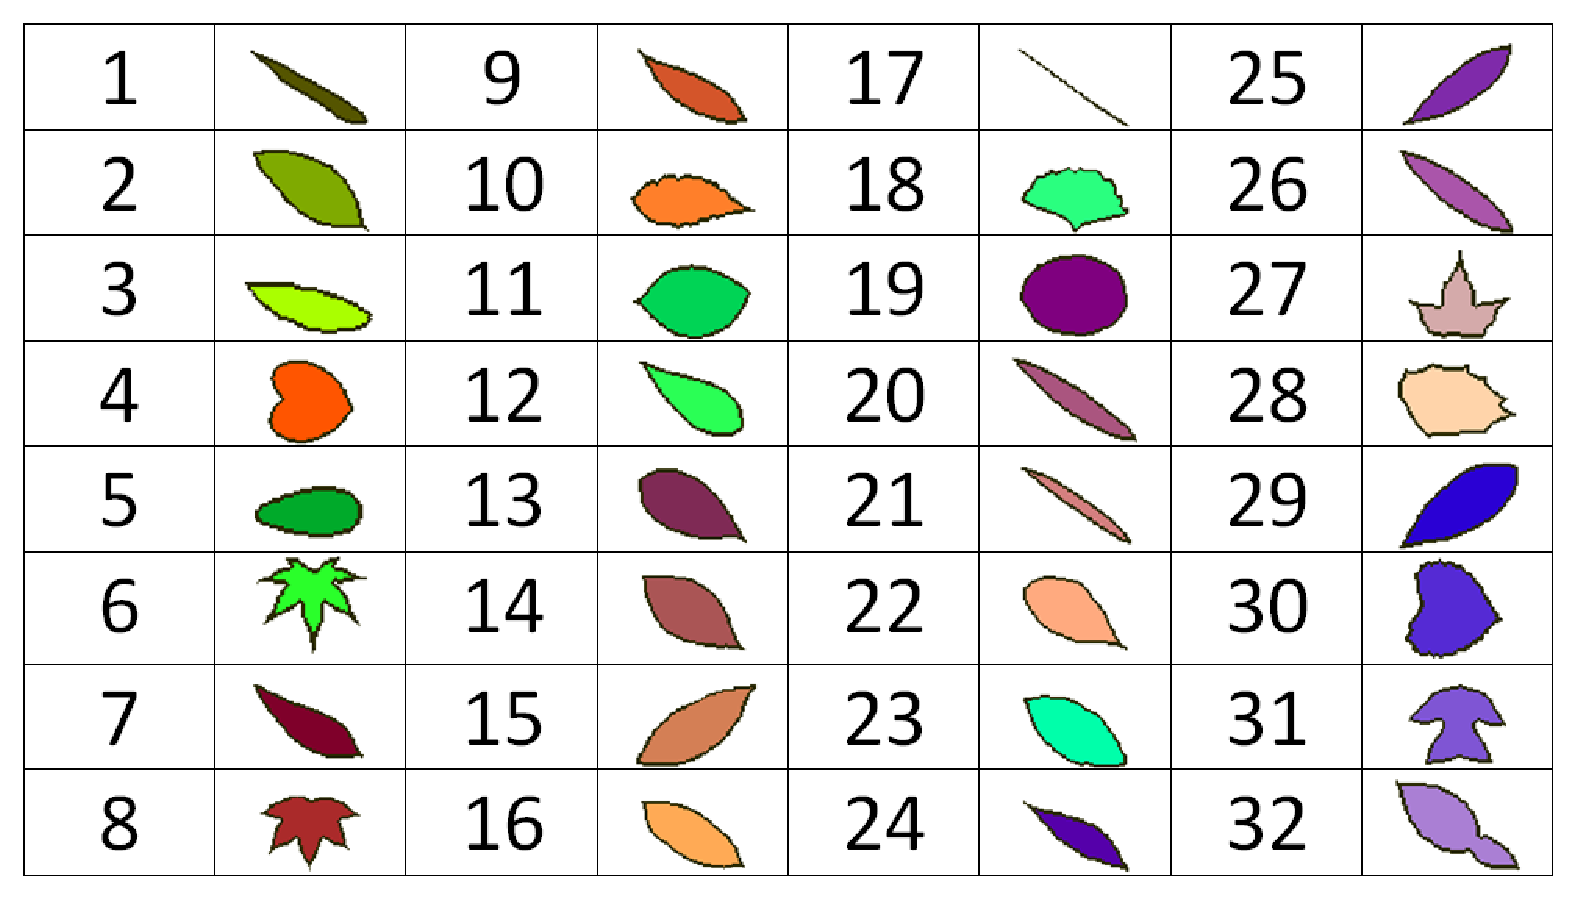
\includegraphics[width=0.5\textwidth]{fig5.eps}
\end{figure}




\section{\emph{Classificação de formas e sua relação com  a função objetivo}}
Nos experimentos realizados para comparação dos algoritmos de otimização, avaliamos inicialmente aspectos  relacionados à  convergência dos algoritmos de otimização e a relação entre os resultados de classificação e as funções \ac{MAD}s obtidas por diferentes estratégias. Além disso investigamos o custo computacional dos mesmos. A Figura \ref{fig:converge} ilustra a convergência de cada um dos três algoritmos de otimização para $30$ repetições realizadas em um subconjunto da base de formas de folhas de plantas. Os resultados obtidos indicam que a otimização realizada pelo \ac{PSO} requereu um pequeno número de iterações para convergir a uma solução ótima, quando comparado aos algoritmos \ac{SA} e \ac{DE}. Uma vez que a convergência está relacionada com o número de iterações necessárias para se atingir uma solução ótima, um menor número de iterações implica em exploração deficiente do espaço de busca, ou seja, em convergência prematura \citeonline{Andries:2007}. Nestes casos, o método de otimização apresenta tendência de ficar preso a mínimos locais, encontrando assim soluções sub-ótimas para o problema. Por outro lado, a convergência mais lenta permite ao algoritmo explorar melhor o espaço de busca, aumentando portanto a chance deste convergir para um mínimo global, ou seja, uma solução ótima \citeonline{Andries:2007}.
 
Neste contexto, observa-se na Figura \ref{fig:converge}c que o \ac{PSO} encontrou soluções sub-ótimas com maior frequência, alcançando valores médios da função \ac{MAD}  igual a $0,805 \pm 0,006$.  Com relação aos algoritmos \ac{SA} e \ac{DE}, estes alcançaram os menores valores médios de \ac{MAD} : $0,795 \pm 0,006$ e $0,798 \pm 0,004$, respectivamente. Esses resultados demonstram que os algoritmos \ac{SA} e \ac{DE} foram mais eficazes que o \ac{PSO} em encontrar soluções ótimas. No entanto, o custo para alcançar tais soluções torna-se maior. A Seção \ref{sec:comp_cost} aborda com mais detalhes as questões relativas ao custo computacional dos algoritmos de otimização utilizados.

\begin{figure}[!htb]
\caption{\label{fig:converge} Convergência dos métodos de otimização para o problema de descrição de folhas de plantas: (a) \ac{SA}, (b) \ac{DE}, (c) \ac{PSO}. As curvas em vermelho destacam o valor médio da função \ac{MAD} para $30$ realizações de cada método (curvas em preto).} 

\includegraphics[width = \textwidth]{converge.jpg}
\end{figure}

A análise corrente tem como hipótese o fato de que as escalas otimizadas e o valor ótimo de \ac{MAD}, que estão inter-relacionadas, implicam em melhorias na taxa de acerto da classificação das espécies vegetais. A Tabela \ref{tab:leaves_supervised_results} exibe os diversos valores de \ac{MAD} e os correspondentes resultados obtidos nos experimentos de classificação para diferentes classificadores. Observa-se que os melhores resultados de classificação correspondem aos menores valores de \ac{MAD} obtidos através da metodologia de otimização de parâmetros. Os resultados de classificação para o descritor \ac{NMBE}, com as escalas ajustadas conforme sugerido por \citeonline{Costa:1997} ($\operatorname{NMBE_{orig}}$), resultou em um desempenho intermediário quando comparado aos resultados para escalas otimizadas e escolhidas arbitrariamente. Os resultados mostram que o descritor \ac{NMBE} otimizado ($\operatorname{NMBE_{opt}}$) melhorou o desempenho de todos os classificadores avaliados, uma vez que este alcançou as maiores taxas de Precisão e Revocação para os menores valores de \ac{MAD}, o que confirma a hipótese inicial.

Apesar do descritor \ac{NMBE} ter sido originalmente projetado para descrição de formas de neurônios, nesta tese o aplicamos com sucesso em caracterização de folhas de plantas, uma vez que a metodologia de otimização o ajustou ao problema em questão.
É importante ressaltar que os diferentes algoritmos de otimização, atingiram valores de \ac{MAD} distintos, e portanto conjuntos de escalas otimizadas distintos, os resultados de classificação corroboraram a hipótese e a conclusão anterior, pois tais conjuntos de escalas  permitiram que os descritores fossem capazes de capturar detalhes dos contornos das formas e as diferenciasse apropriadamente. Com isso, observamos que os algoritmos de otimização trazem vantagens à representação multiescala com impacto significativo na caracterização das folhas. 

\begin{table}[]
\begin{minipage}{\textwidth}
\renewcommand\footnoterule{}
\caption{Valores de \ac{MAD} e resultados de classificação das espécies vegetais da base de imagens Flavia para diferentes estratégias de escolha das escalas do descritor \ac{NMBE}. }
\label{tab:leaves_supervised_results}
\resizebox{\textwidth}{!}{ 
\begin{tabular}{cccccccccc}
\toprule[1.5pt]
 & \multicolumn{8}{c}{Classifier} \\ \cmidrule(lr){2-9} 
 & \multicolumn{2}{c}{NB}  & \multicolumn{2}{c}{Knn (n = 5)}  & \multicolumn{2}{c}{LDA}  & \multicolumn{2}{c}{QDA} \\
\cmidrule(lr){2-3}  \cmidrule(lr){4-5} \cmidrule(lr){6-7}  \cmidrule(lr){8-9}
\ac{MAD} & Precision & Recall & Precision & Recall & Precision & Recall & Precision & Recall \\ \midrule
$0,762$\footnote{Using \ac{SA}}        & ${0,91 \pm 0,02}$   & ${0,89 \pm 0,02}$         & ${0,93 \pm 0,02}$          & ${0,92 \pm 0,02}$         & ${0,87  \pm 0,02}$          & ${0,85\pm 0,02}$         & ${0,95  \pm 0,01}$          & ${0,94  \pm 0,01}$         \\
$0,783$\footnote{Using \ac{DE}}        & $0,88 \pm 0,02$          & $0,87\pm0,02$         & $0,90\pm0,02$          & $0,88\pm0,02$         & $0,85\pm0,02$          & $0,83\pm0,03$         & $0,91\pm0,02$          & $0,90\pm0,02$         \\
$0,829$\footnote{Using \ac{PSO}}        & $0,86\pm0,03$          & $0,85\pm0,03$         & $0,89\pm0,03$          & $0,88\pm0,03$         & $0,84\pm0,03$         & $0,82\pm0,03$         & $0,91\pm0,02$          & $0,89\pm0,02$         \\
{$0,867$\footnote{Using scales proposed by \citeonline{Cesar:1996}}}          & $0,85\pm0,02$          & $0,84\pm0,02$         & $0,89\pm0,02$          & $0,88\pm0,02$         & $0,82\pm0,03$          & $0,81\pm0,03$         & $0,89\pm0,02$          & $0,88\pm0,02$         \\
{$0,969$\footnote{\label{note1}Random selection}}          & $0,81\pm0,03$          & $0,79\pm0,03$         & $0,87\pm0,02$          & $0,85\pm0,02$         & $0,77\pm0,03$          & $0,77\pm0,03$         & $0,87\pm0,03$          & $0,85\pm0,03$         \\
{$1,04$\footref{note1}}          & $0,69\pm0,03$          & $0,68\pm0,03$         & $0,83\pm0,03$          & $0,82\pm0,03$         & $0,74\pm0,03$          & $0,73\pm0,03$         & $0,81\pm0,03$          & $0,79\pm0,03$         \\
\bottomrule[1.5pt]
\end{tabular}}
\end{minipage}
\end{table}
  
Os resultados da Tabela \ref{tab:leaves_supervised_results} confirmam que os classificadores que utilizaram descritores gerados a partir de escalas selecionadas arbitrariamente não tiveram desempenho satisfatório, pois alcançaram os menores valores de Precisão e Revocação e os maiores valores da função \ac{MAD}. Portanto, escalas aleatórias levam a uma representação multiescala menos sensível a variações de características das folhas, consequentemente, mais erros de classificação. 

\section{\emph{Análise exploratória visual de agrupamentos}}

Nesta seção utilizamos técnicas de visualização de dados multidimensionais, como \ac{MDS} e matriz-U, para observar os resultados dos descritores multiescala \ac{NMBE} e \ac{DFM}. O uso dessas técnicas suportam a análise do comportamento dos descritores a partir de suas relações com os agrupamentos observados em um espaço bidimensional. 

%As três imagens na Figura \ref{fig:nuvem_pca} representam projeções bidimensionais das duas primeiras componentes principais (mais relevantes) dos vetores de características obtidos a partir dos descritores \ac{NMBE} e \ac{DFM} transformados através da \emph{PCA}, assim como a combinação de ambos. Os números anotados dentro dos gráficos indicam a acurácia média por classe. Visualmente as projeções das duas componentes indicam a complexidade do problema da análise de formas, a dimensionalidade do problema e a dificuldade em projetar descritores e ajustar seus parâmetros de modo que descrevam as mais diversas nuances de formas de bases de uso geral (Kimia-99, Kimia-216, MPEG7 CE-Shape-1) e aplicadas (Flavia). Observa-se que a qualidade dos agrupamentos em geral não é boa para todas as classes, quando se aplica \ac{NMBE} e \ac{DFM}, entretanto a combinação de ambos os descritores elevou a qualidade da discriminação das formas e da recuperação das mesmas.  

%\begin{figure}[t]
%  \caption{\label{fig:nuvem_pca} Imagens das projeções das duas primeiras componentes principais, obtidas através de PCA, dos vetores de características transformados para os descritores \ac{NMBE} e  \ac{DFM} individualmente e combinados.}
%  \centering
%  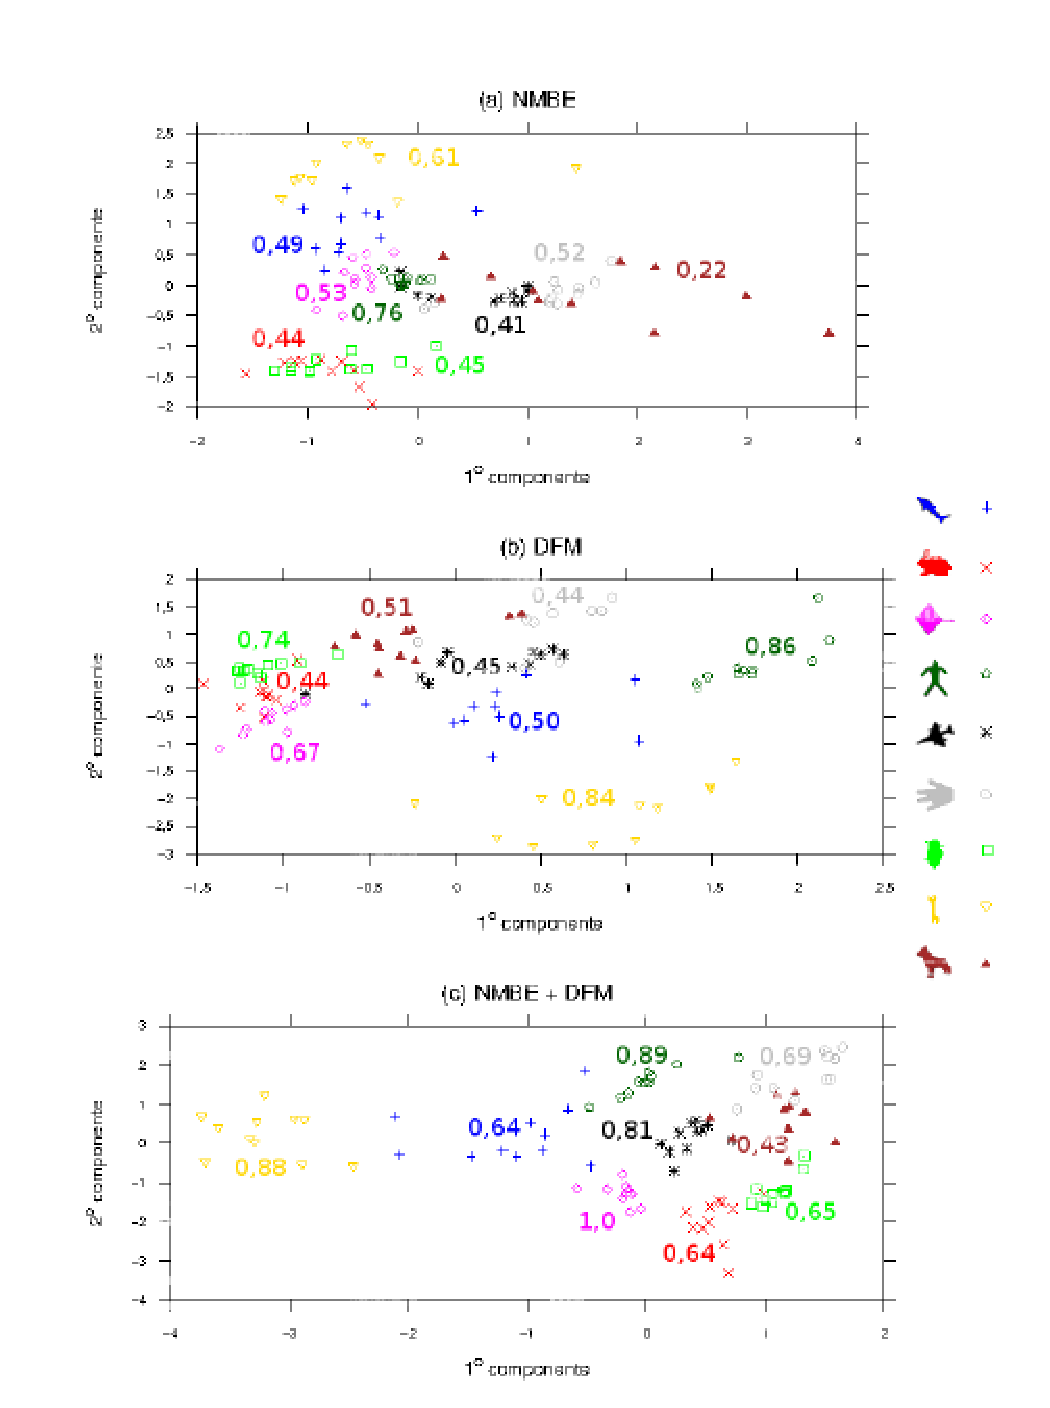
\includegraphics[width=0.75\textwidth]{nuvem_pca.eps}
%\end{figure}

\begin{figure}[t]
 \caption{\label{fig:nmbe_dfm_99} Resultados dos descritores \ac{NMBE} e \ac{DFM} para a base Kimia-99. (a) Matriz-U obtida com o descritor \ac{NMBE} e respectiva \textit{Silhouette} média por classe. (b) Matriz-U obtida com o descritor \ac{DFM} e respectiva \textit{Silhouette} média por classe.}
  \centering
  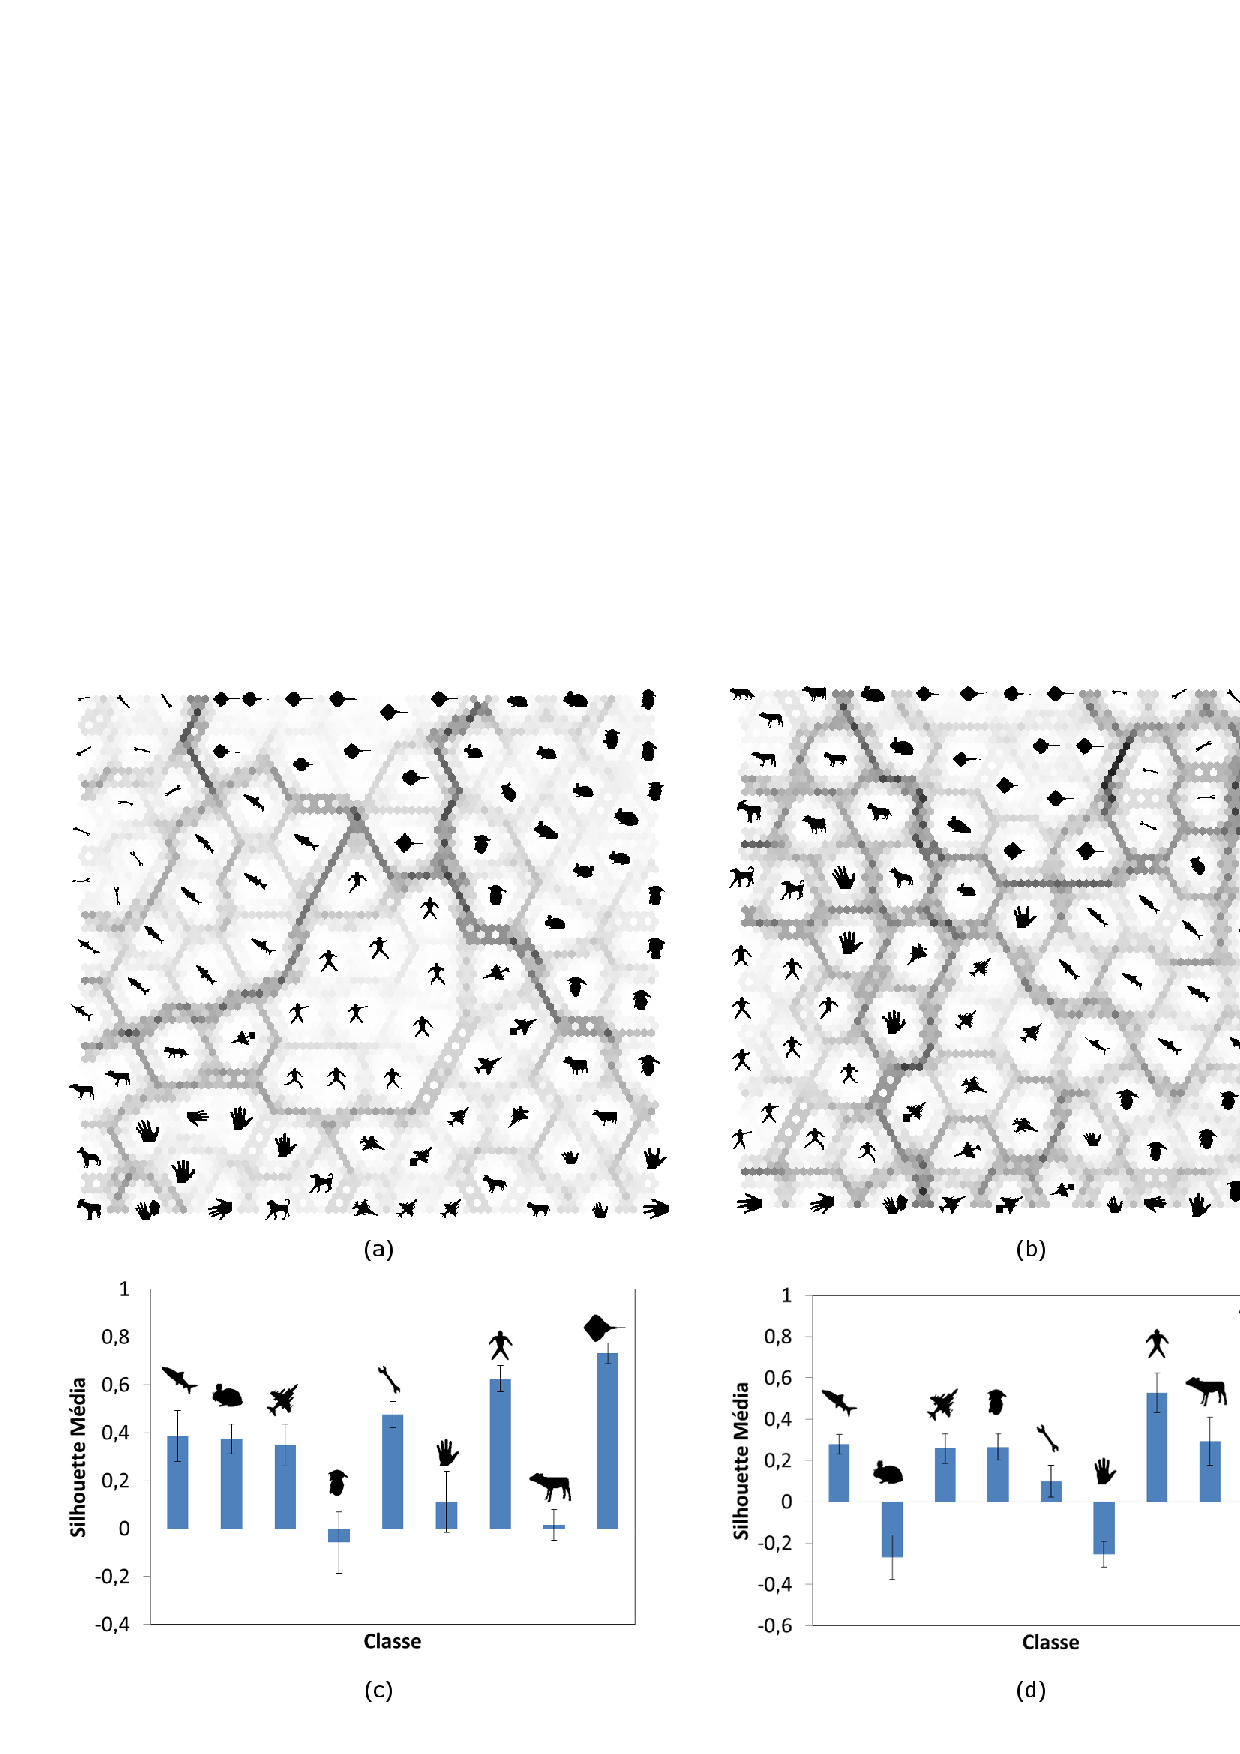
\includegraphics[width=\textwidth]{nmbe_dfm_99.jpg}
\end{figure}

\begin{figure}[t]
 \caption{\label{fig:nmbe_dfm_216} Resultados dos descritores \ac{NMBE} e \ac{DFM} para a base Kimia-216. (a) Matriz-U obtida com o descritor \ac{NMBE} e respectiva \textit{Silhouette} média por classe. (b) Matriz-U obtida com o descritor \ac{DFM} e respectiva \textit{Silhouette} média por classe.}
  \centering
  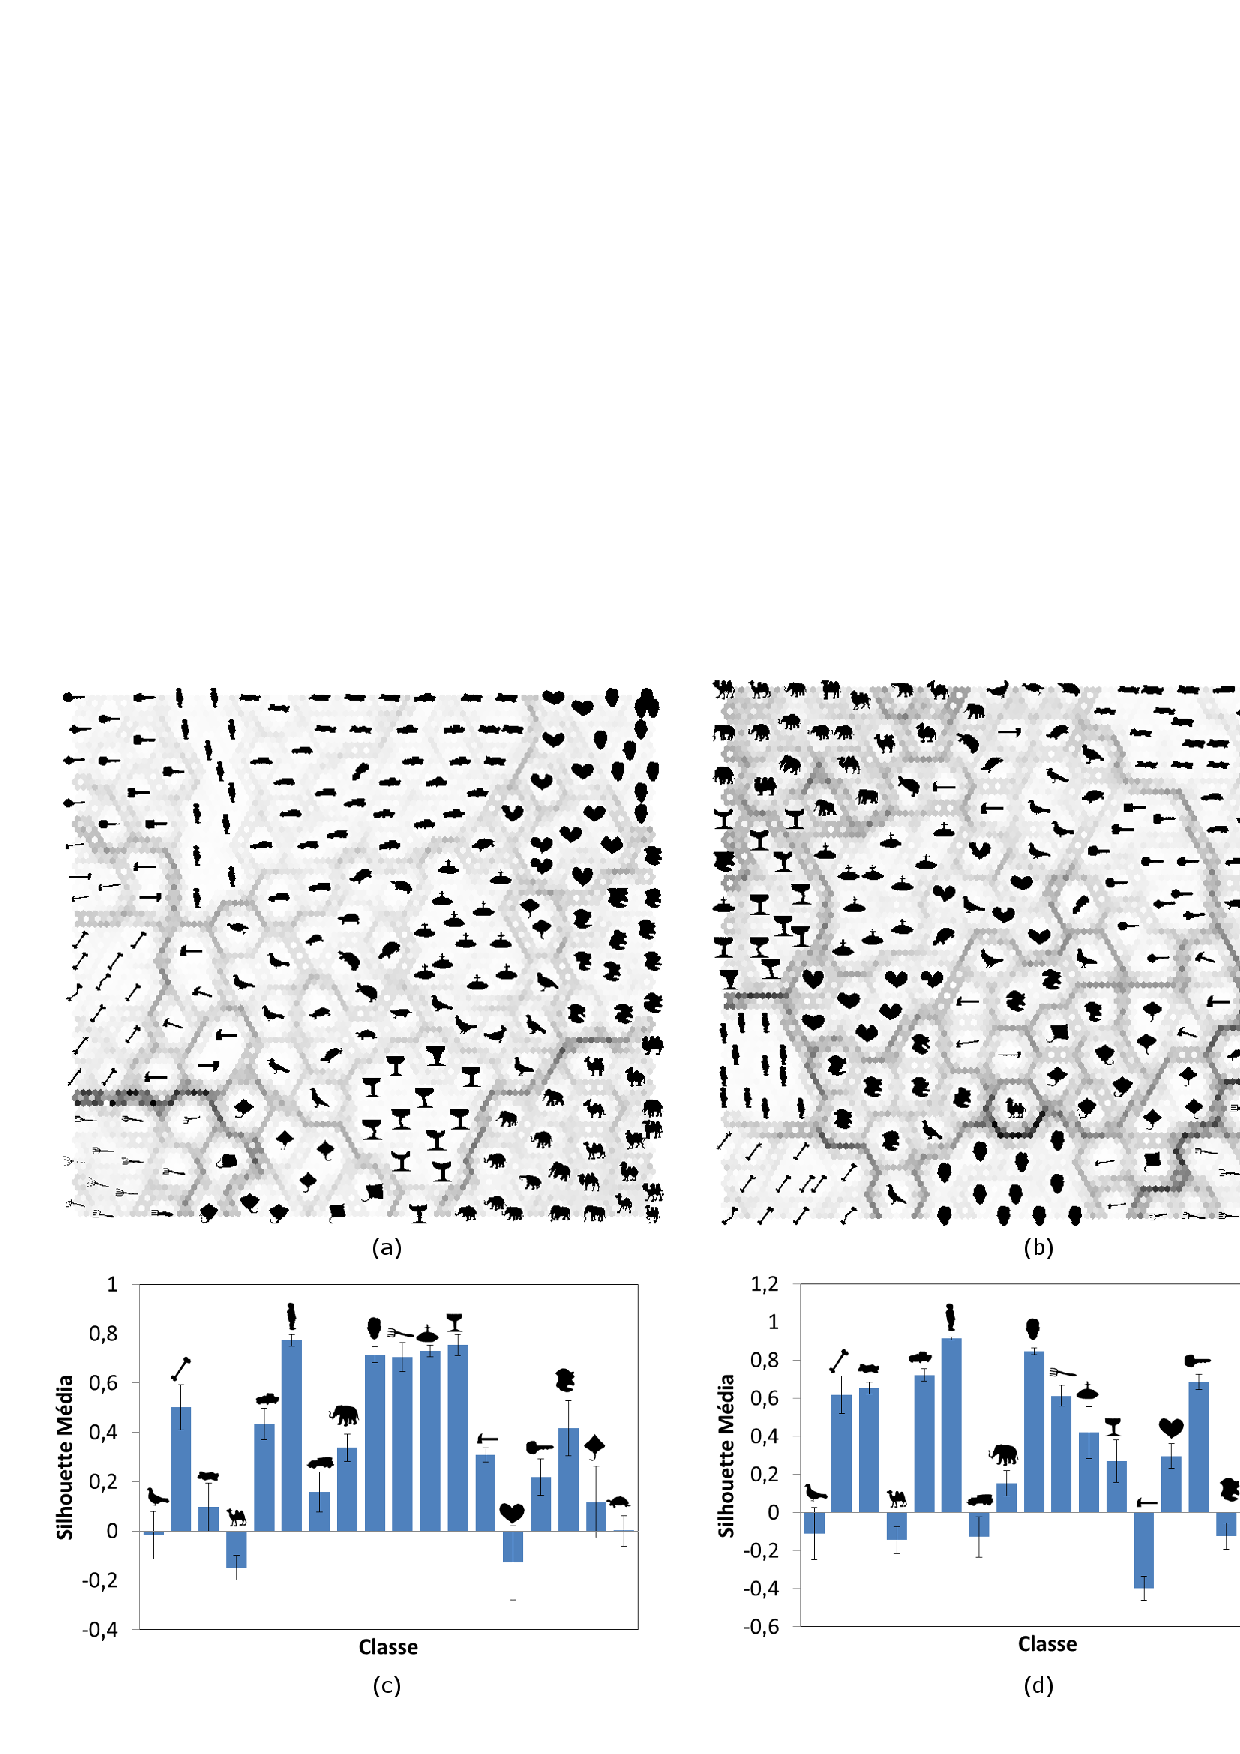
\includegraphics[width=\textwidth]{nmbe_dfm_216.jpg}
\end{figure}

Para ilustrar o poder discriminativo dos descritores de forma multiescala \ac{NMBE} e \ac{DFM}, bem como mostrar a relação existente entre a medida de avaliação quantitativa da qualidade dos agrupamentos, \emph{silhouette}, e a representação qualitativa obtida através da matriz U, foram realizadas as extrações de características das formas das bases Kimia-99 e Kimia-216 com os referidos descritores. Os resultados estão expostos nas Figuras \ref{fig:nmbe_dfm_99} e \ref{fig:nmbe_dfm_216}. 

Em ambas as figuras, observa-se que as formas correspondentes às classes com  \emph{silhouette} média positiva são visualizadas na matriz-U mantendo forte relação de vizinhança entre si, enquanto que formas correspondentes às classes cuja \emph{silhouette} média é negativa encontram-se dispersas nessas matrizes. Isso denota a inabilidade da descrição  em representá-las adequadamente.

Assim, os descritores conseguem capturar características tanto globais como locais, uma vez que classes de formas com características globais semelhantes, como por exemplo as formas alongadas do canto superior esquerdo da Figura \ref{fig:nmbe_dfm_216}a, estabelecem uma relação de vizinhança entre si. Apesar disso, formas alongadas de classes distintas não se misturam, o que é um indicativo de que o descritor foi capaz também de representar características locais discriminativas que permitem a separação entre as classes.

Existem no entanto casos, em que ambos os descritores não foram capazes de discriminar formas com características globais semelhantes, como é o caso das classes de formas de elefantes e camelos na Figura \ref{fig:nmbe_dfm_216}. Na matriz-U, estas formas aparecem agrupadas como se pertencessem a uma mesma classe e consequentemente, com valores de \emph{silhouette} média significativamente menores em relação às formas que foram discriminadas corretamente pelos descritores.

A Figura \ref{fig:MatrizU_leaves_256}a mostra a matriz-U obtida para as formas de folhas de plantas da base Flavia representadas pelo descritor \ac{NMBE} otimizado e a Figura \ref{fig:MatrizU_leaves_256}b, pelo descritor \ac{NMBE} não otimizado. A análise exploratória visual dos agrupamentos produzidos pela descrição \ac{NMBE} indica que a descrição otimizada melhora a organização dos agrupamentos. Essa evidência então confirma que a função objetivo \ac{MAD} é adequada para guiar o processo de otimização desse descritor. A visualização das formas nas matrizes-U da Figura \ref{fig:MatrizU_leaves_256}  aponta diferenças entre os dois arranjos promovidos pelos referidos descritores. A cada posição ou elemento da matriz, os valores numéricos foram substituídos pela imagem das folhas correspondentes, estando as cores das folhas em correspondência com o rótulo das classes exibidas na Figura \ref{fig:bases}. Nessas matrizes-U estão representadas as $1907$ formas de folhas da base Flavia, sendo cada folha representada por sua descrição multiescala.

Os gráficos representativos da \emph{silhouette} média nas  Figura \ref{fig:MatrizU_leaves_256}a  e Figura \ref{fig:MatrizU_leaves_256}b demonstram que as classes das folhas bem caracterizadas e, portanto, agrupadas adequadamente são as que apresentam valores de \emph{silhouette} média positivos. Por outro lado, as classes de folhas que o descritor não foi capaz de caracterizar e agrupar adequadamente são as que apresentaram valores negativos de \emph{silhouette} média. Comparando estes resultados, observa-se que na Figura \ref{fig:MatrizU_leaves_256}a há expressiva redução dos valores negativos de \emph{silhouette} média quando se utiliza o descritor $\operatorname{NMBE_{opt}}$. 

\begin{figure}[t]

\caption{\label{fig:MatrizU_leaves_256} Matrizes-U e a \emph{silhouette} média para as descrições das folhas da base Flavia com o descritor \ac{NMBE} (a) optimizado e (b) não otimizado.}
\centering
\includegraphics[width=\textwidth]{Umat_leaves.jpg}

\end{figure}

O quadrado preto inserido na Figura \ref{fig:MatrizU_leaves_256} destaca o desempenho do descritor otimizado em termos de melhoria no arranjo das formas na matriz-U. É possível ainda observar quão bem o descritor otimizado mapeou as folhas em grupos de acordo com as respectivas classes rotuladas das mesmas.  Além do mais, o resultado com as escalas otimizadas melhorou significativamente a \emph{silhouette} média por classe para quase todas as classes de folhas da base. Por outro lado, a região interna ao quadrado preto na Figura \ref{fig:MatrizU_leaves_256}b destaca que o descritor não otimizado não foi capaz de mapear satisfatoriamente as formas de  folhas em suas classes correspondentes. Deduzimos que essa melhoria se deve ao fato de que as escalas otimizadas dos descritores são mais sensíveis a variações intrínsecas das formas, ou sejam, incorporam nuances presentes nos seus contornos, os quais os métodos tradicionais não o fazem adequadamente. Além do mais, o ajuste automático das escalas é de fato uma tarefa alternativa para o ajuste arbitrário ou empírico, sendo que esta última não é uma tarefa simples e está sujeita à fadiga e subjetividade do realizador da mesma.


As Figuras \ref{fig:MatrizU_leaves_II}a, \ref{fig:MatrizU_leaves_II}b and \ref{fig:MatrizU_leaves_II}c exibem as matrizes-U correspondentes aos valores \ac{MAD} dos experimentos na base Flavia utilizando os algoritmos de otimização \ac{SA}, \ac{DE} e \ac{PSO}, respectivamente. Um aspecto interessante a examinar é o fato dos três algoritmos apresentarem diferentes soluções, ou valores de \ac{MAD}. Estas soluções resultaram em diferentes arranjos de folhas e consequentemente diferentes relações entre as estruturas de vizinhança dos grupos ou classes.
Por exemplo, a dispersão geral dos elementos nas Figuras \ref{fig:MatrizU_leaves_II}a e \ref{fig:MatrizU_leaves_II}b tende a ser muito semelhante uma vez que seus respectivos valores da função objetivo minimizada são bem próximos em magnitude. Ao mesmo tempo, concluímos que o resultado que corresponde ao mais elevado valor de \ac{MAD} ($0,829$) exibe uma dispersão particularmente elevada no centro da Matriz-U (Figura \ref{fig:MatrizU_leaves_II}c). Este é um detalhe que reforça a observação anterior de que o \ac{PSO} convergiu para um mínimo local. 
Estes achados apontam para a importante conclusão de que quanto menor o valor de \ac{MAD}, melhor o arranjo dos grupos ou do agrupamento, e consequentemente a qualidade do agrupamento. Por isso, afirmamos que a qualidade dos grupos e o valor de \ac{MAD} são negativamente correlacionados. Nossa análise ainda considera que devam existir outras soluções no espaço de busca, além da solução mínima, que sejam adequadas ao problema em estudo.

\begin{figure}[h!] \caption{\label{fig:MatrizU_leaves_II}Matrizes-U e valores \ac{MAD}s obtidos para a base de imagens Flavia por uso da \ac{NMBE} otimizada pelos algoritmos (a) \ac{SA}, (b) \ac{DE}, (c) \ac{PSO}.}
\centering
\includegraphics[width=\textwidth]{Umat_SA_DE_PSO_v2.jpg}
\end{figure}

A Figura \ref{MDS:Leaves} ilustra as projeções \ac{MDS} para três valores distintos de \ac{MAD}. Na Figura \ref{MDS:Leaves}a temos o arranjo dos agrupamentos após a convergência do algoritmo de otimização \ac{SA}, ou seja, para o descritor cujos parâmetros otimizados correspondem ao mínimo valor da função \ac{MAD} encontrado nas otimizações. Analisando essas projeções, observa-se que a minimização da função objetivo resultou em agrupamentos de folhas com maior coesão intra classe e maior separação entre classes. A análise visual das três regiões detalhadas  nessa imagem indica mais claramente que o descritor \ac{NMBE} otimizado melhorou a representação das formas de folhas em comparação aos resultados das Figuras \ref{MDS:Leaves}b e \ref{MDS:Leaves}c. Ademais, os valores do coeficiente $R^2$ próximos de $1,0$ indicam que a representação no espaço bi-dimensional preservou a relação de distâncias entre as amostras no espaço de alta dimensão.

\begin{figure}[t]
 \caption{\label{MDS:Leaves} Projeções \ac{MDS} dos descritores \ac{NMBE} para formas da base de folhas Flavia. (a) Descritor \ac{NMBE} otimizado pelo algoritmo \ac{SA} com valor de função $\ac{MAD} = 0,762$ (b) Descritor \ac{NMBE} não otimizado com valor de função $\ac{MAD} =0,969$ and (c) Descritor \ac{NMBE} não otimizado com valor de função $\ac{MAD} = 1,044$.}

\centering
\includegraphics[width=\textwidth]{MDS_Leaves.jpg}
\end{figure}

\section{Recuperação de imagens baseada em conteúdo}

O descritor \ac{IDSC} \cite{Ling:2007:SCU:1191552.1191806} foi otimizado para fins de comparação com o descritor multiescala. Desenvolvido para aplicações de recuperação de formas, o \ac{IDSC} utiliza algoritmos de programação dinâmica, tal como o \ac{DTW} \cite{PalazonGonzalez2012978}, para melhorar a precisão da avaliação de similaridade entre formas. Assim sendo, subsituimos a norma $L_2$ pelo algoritmo \ac{DTW} no cálculo da medida \emph{silhouette}, uma vez que esta última é requerida para a avaliação da função objetivo \ac{MAD} na Equação \ref{eq:mad}. 

A Figura \ref{fig1Ooptimization_graph}a exibe gráficos que permitem a comparação dos resultados dos experimentos realizados para as versões otimizadas ($\operatorname{NMBE_{opt}}$, $\operatorname{IDSC_{opt}}$)
 e não otimizadas ($\operatorname{NMBE}$, $\operatorname{IDSC}$) de ambos descritores. Os gráficos mostram que o ajuste dos parâmetros dos descritores pelo método de otimização melhorou o resultado (taxa) de recuperação de folhas consideravelmente. Observamos ainda que o descritor $\operatorname{IDSC_{opt}}$ superou ambos os descritores $\operatorname{NMBE_{opt}}$ e \ac{NMBE} não otimizado com relação à taxa de recuperação. Logo, podemos afirmar que a otimização de parâmetros melhorou a capacidade de discriminação do  $\operatorname{IDSC_{opt}}$, incorporando ao descritor um mecanismo de extração de informações relevantes de detalhes intrínsecos das formas das folhas. Por outro lado, observamos que o desempenho do \ac{IDSC} não otimizado foi inferior ao do \ac{NMBE} não otimizado. 

As Figuras \ref{fig1Ooptimization_graph}b e \ref{fig1Ooptimization_graph}c ilustram resultados obtidos de recuperação de dois exemplares da base de imagens de folhas para experimentos realizados com os descritores \ac{NMBE} não otimizado e $\operatorname{NMBE_{opt}}$,  \ac{IDSC} não otimizado com parâmetros ajustados conforme recomendado em \cite{wang2015march} e $\operatorname{IDSC_{opt}}$. Observa-se na Figura \ref{fig1Ooptimization_graph}b que o descritor \ac{NMBE} não otimizado falhou parcialmente na recuperação das formas, enquanto a versão otimizada ($\operatorname{NMBE_{opt}}$) com sucesso recuperou todas as formas. O mesmo comentário se aplica ao descritor $\operatorname{IDSC_{opt}}$, cujos resultados mostram o sucesso da recuperação. Ainda na Figura \ref{fig1Ooptimization_graph}c, o descritor \ac{IDSC} não otimizado não foi capaz de recuperar as amostras corretamente.

\begin{figure}[]
\caption{Experimentos realizados com formas da base de imagens de folhas Flavia (a) taxa de recuperação  obtida com os descritores \ac{NMBE} e \ac{IDSC} originais e suas versões otimizadas, (b) e (c) recuperação de duas amostras de folhas utilizando os descritores \ac{NMBE} e \ac{IDSC} otimizados e não otimizados, respectivamente.\label{fig1Ooptimization_graph}}
\includegraphics[width=\textwidth]{res_cbir.jpg}
\end{figure}

\begin{comment}
\begin{figure}[t!]
\begin{subfigure}{0.55\textwidth}
\includegraphics[width=\textwidth]{fig10a.eps}
\caption{Retrieval rates. \label{fig1Ooptimization_graph}}
\end{subfigure}
\hspace*{\fill}
\begin{minipage}{0.45\textwidth}
\begin{subfigure}{\textwidth}
\includegraphics[width=\textwidth]{fig10b.eps}
\caption{Retrieval results with \ac{NMBE}.} \label{subfig:upper-right}

\end{subfigure}

\vspace*{0.60cm}
\begin{subfigure}{\textwidth}
\includegraphics[width=\textwidth]{fig10c.eps}
\caption{Retrieval results with \ac{IDSC}.\label{subfig:lower-right}}
\end{subfigure}
\end{minipage}

\caption{\label{figfig1Optmization-IDSC} Experiments conducted on Flavia leaf data set (a) retrieval rate by using both \ac{NMBE} and \ac{IDSC} and their optimized counterparts, (b) and (c) two leaf shape retrieval examples by using the non-optimized and optimized \ac{NMBE} and \ac{IDSC} descriptors, respectively.} 
\end{figure}
\end{comment}

A Tabela \ref{table_bull_eyes_leaves} apresenta o resultado da avaliação de desempenho dos descritores $\operatorname{NMBE_{opt}}$ e \ac{NMBE} não otimizado com escalas ajustadas conforme recomendado em \cite{Cesar:1996},  $\operatorname{IDSC_{opt}}$ e o \ac{IDSC} não otimizado. Esses resultados mostram que a taxa de recuperação para ambos os descritores otimizados superou os resultados dos pares correspondentes não otimizados. A melhoria significativa observada nas medidas Bulls-eye reforça a hipótese de que a metodologia de otimização proposta é adequada para ajuste dos descritores em aplicações de recuperação e análise de formas de folhas.

\begin{table}[h!]
\centering
\caption{Taxa Bulls-eye para a base de imagens Flavia.}
\label{table_bull_eyes_leaves}
  \begin{tabular}{cccccccc}
  \toprule[1.5pt]
 $\operatorname{\ac{NMBE}}$ & $\operatorname{NMBE_{opt}}$ & \ac{IDSC}    & $\operatorname{IDSC_{opt}}$\\ \midrule
     63.86 \%  & 71.16 \%  & 53.38\%    & 77.50\%       \\
  \bottomrule[1.5pt]
  \end{tabular}
\end{table}

\section{Custo computacional da otimização \label{sec:comp_cost}}


 Nesta tese avaliamos a complexidade computacional dos três algoritmos de otimização como exibe a Tabela \ref{tbl:complexity}.  Os algoritmos \ac{SA} e \ac{PSO} apresentam complexidades similares e estas dependem do número de iterações para convergir ($N_{iter}$), do tamanho da população  ($N_{pop}$) e do parâmetro $P$.  Por outro lado, o algoritmo \ac{DE} demanda maior complexidade, pois depende da dimensão ($D$) do problema a ser otimizado, do tamanho da população ($N_{pop}$) e do número de interações ($N_{iter}$).

\begin{table}[h!]
\centering
\caption{Complexidade computacional dos métodos de otimização.}
\label{tbl:complexity}
  \begin{tabular}{ll}
  \toprule[1.5pt]
 Método & Complexidade\\
 \midrule
   \ac{SA}  & $O(P.N_{iter}.\log{N_{iter}})$    \\
   \ac{DE}  & $O(N_{pop}.N_{iter}.D)$   \\
   \ac{PSO}&  $O(N_{pop}.N_{iter}.\log{N_{iter}})$\\
  \bottomrule[1.5pt]
  \end{tabular}
\end{table}

Para fins de comparação dos métodos de otimização, sob o aspecto de custo computacional, assumimos o custo computacional dos algoritmos como sendo o número de vezes que a função objetivo é demandada ao longo do processo de otimização. Considerando para cada método de otimização o ajuste de parâmetros adotado, bem como a complexidade computacional correspondente, os custos computacionais calculados para os algoritmos \ac{SA}, \ac{DE} e \ac{PSO} resultaram em $7.4314$, $19.500$ e $1.107$, respectivamente. 

Vale destacar que existe um compromisso entre o custo computacional e a qualidade da solução ótima obtida. Assim sendo a redução do número de amostras de formas, da resolução das imagens e do tamanho da população dos métodos ($N_{pop}$) ameniza o custo computacional, porém estas reduções degradam a qualidade do resultado da otimização. Ademais, o uso de processamento paralelo pode contribuir para a redução do custo computacional, sem degradar a qualidade da solução ótima, entretanto o paralelismo adiciona complexidade aos algoritmos de otimização. 



\begin{comment}
\begin{figure}
 \caption{\label{fig:edif99} (a) Matriz-U para as formas da base Kimia99 representadas com o descritor entropia multiescala. (b) Silhouette média por classe aferida a partir do descritor}
  \centering
  \includegraphics[width=\textwidth]{ediferencial99.png}
\end{figure}

\begin{figure}
 \caption{\label{fig:edif216} (a) Matriz-U para as formas da base Kimia216 representadas com o descritor entropia multiescala. (b) Silhouette média por classe aferida a partir do descritor}
  \centering
  \includegraphics[width=\textwidth]{ediferencial216.png}
\end{figure}

\begin{figure}
 \caption{\label{fig:edis99} (a) Matriz-U para as formas da base Kimia99 representadas com o descritor entropia multiescala. (b) Silhouette média por classe aferida a partir do descritor}
  \centering
  \includegraphics[width=\textwidth]{ediscreta99.png}
\end{figure}

\begin{figure}
 \caption{\label{fig:edis216} (a) Matriz-U para as formas da base Kimia216 representadas com o descritor entropia multiescala. (b) Silhouette média por classe aferida a partir do descritor}
  \centering
  \includegraphics[width=\textwidth]{ediscreta216.png}
\end{figure}

\subsection{\ac{NMBE} e \ac{DFM}}
Os experimentos de avaliação de desempenho dos descritores produziram como saída as matrizes-U que estão apresentadas na Figuras \ref{fig:nmbe_som_map}, \ref{fig:mfd_som_map} e  \ref{fig:som_kimia_216}. Nas Figuras \ref{fig:nmbe_som_map} e \ref{fig:mfd_som_map}, as regiões delimitadas com linhas tracejadas correspondem as classes de formas com os maiores valores médios da medida Silhouette (Figuras \ref{fig:silhouette}a e \ref{fig:silhouette}b). Nesses casos pode-se deduzir que ambos os descritores foram capazes de caracterizar corretamente estas classes de formas.

Já os grupos delimitados com linhas contínuas referem-se às classes de formas com os menores valores de Silhouette média. De fato, as formas dessas classes aparecem nas matrizes-U dispersas em sub-grupos, que é um indicativo que ambos os descritores falharam em caracterizá-las adequadamente.
  
As Figuras \ref{fig:dude_tool_mfd} e \ref{fig:dude_tool_nmbe} mostram objetos das classes de formas de humanos e ferramentas. Ambos os descritores foram capazes de discriminar os objetos das referidas classes, como evidenciado nos gráficos apresentados. As matrizes-U (Figuras \ref{fig:nmbe_som_map} e \ref{fig:mfd_som_map}) também confirmam esse resultado exibindo, para essas classes de formas, homogeneidade intra-classe e separabilidade inter-classes. Logo, concluímos que estes descritores são efetivos em representar formas para o reconhecimento de padrões em aplicações \ac{CBIR}.

Também evidenciamos nas Figuras \ref{fig:mfd_som_map} e \ref{fig:nmbe_som_map} que o descritor \ac{DFM} apresentou maior dispersão inter-classe para as formas de humanos que o descritor \ac{NMBE}. Essa observação é consistente com os resultados obtidos através da medida \emph{Silhouete}, aonde o valor dessa medida para formas humanas descritas com a \ac{DFM} é menor do que o valor para essas mesmas formas descritas com a \ac{NMBE}.

Ademais, os sinais em linhas tracejadas vermelhas e em linhas contínuas azuis, apresentados nas Figuras \ref{fig:dude_tool_mfd} e \ref{fig:dude_tool_nmbe}, mostram que o descritor \ac{NMBE} é mais robusto a diferenças intra-classe que o descritor \ac{DFM}. Nesses gráficos, as formas pertencentes a mesma classe que o descritor representa seguindo um mesmo padrão apresentam-se próximas umas das outras na matriz-U, enquanto as formas que o descritor representa divergindo do padrão são mapeadas na matriz-U distantes dos grupo correspondente. Exemplos desta última condição são as formas humanas rotuladas como $2$ e $4$ nas Figuras \ref{fig:dude_tool_mfd} e \ref{fig:dude_tool_nmbe}.


Furthermore, there is a larger variation among tools descriptions in the graphs of  the figure \ref{fig:descritores}a than the  variations observed in the graphs of the figure \ref{fig:descritores}b. Coherently, the corresponding shapes appears in the U-matrix more dispersed  for the \emph{MFD} description than for the \ac{NMBE} description.

\begin{figure}[h!]
  \caption{\label{fig:nmbe_som_map} Matriz-U para as formas da base Kimia99 representadas com o descritor Energia de dobramento multiescala.}
  \centering
  \includegraphics[width=0.5\textwidth]{nmbe_som_map_v4.eps}
\end{figure}

\begin{figure}[h!]
  \caption{\label{fig:mfd_som_map} Matriz-U para as formas da base Kimia99 representadas com o descritor Dimensão fractal multiescala.}
  \centering
  \includegraphics[width=0.5\textwidth]{mfd_som_map_v3.eps}
\end{figure}
  
\begin{figure}[h!]  \caption{\label{fig:som_kimia_216} Para o descritor energia de dobramento multiescala e a base Kimia-216: (a) Matriz-U. (b) Alguns resultados de recuperação de formas pelo conteúdo.}
  \centering
  \includegraphics[width=0.5\textwidth]{retr_som_kimia216_v2.png}
\end{figure}

Já a Figura \ref{fig:som_kimia_216}a apresenta os resultados da visualização das formas da base Kimia-216 representadas através do descritor \ac{NMBE}. No canto inferior direito desta figura observamos que o descritor confunde formas dos elefantes com as dos camelos. Essa confusão aparece também no experimento de recuperação de formas pelo conteúdo (Figura \ref{fig:som_kimia_216}b), em que uma dentre as formas dos elefantes é utilizada como protótipo para se recuperar as onze formas mais similares ao protótipo na referida base.

Analogamente, no canto superior esquerdo da Figura \ref{fig:som_kimia_216}a, há confusão entre os agrupamentos das formas das faces e dos corações, bem como a presença duma forma de garfo. Na segunda linha da Figura \ref{fig:som_kimia_216}b observamos a presença dessas formas indesejáveis no experimento de recuperação de formas quando uma forma de face é apresentada como protótipo. 

Os demais resultados de recuperação de formas, apresentados na Figura \ref{fig:som_kimia_216}b, também estão coerentes com as observações da matriz-U. Nessa última podemos observar que o grupo das formas das arraias são mapeadas vizinhas aos grupos das formas dos cálices e dos pássaros, o que resulta no aparecimento das formas dessas últimas classes quando se realiza a recuperação de arraias. 

Outro aspecto importante de ser observado é que  grupos de formas com similaridades grosseiras encontram-se mapeados próximos uns dos outros na matriz-U. Formas alongadas, por exemplo, estão organizadas na parte inferior esquerda da Figura \ref{fig:som_kimia_216}a, enquanto formas arredondadas encontram-se na parte superior. Outros exemplos incluem os seguintes grupos: chaves e crianças (esquerda da figura), carros e tijolos, tartarugas e pássaros, cálices e sepulturas. 

\begin{figure}[h!]
  \caption{\label{fig:silhouette} Silhouette média por classe aferida, com a base Kimia-99, para os descritores (a) Dimensão fractal multiescala; (b) Energia de dobramento multiescala.}
  \centering
  \includegraphics[width=0.5\textwidth]{resultado_silhouette.eps}
\end{figure}

\begin{figure}[h!]
  \caption{\label{fig:dude_tool_mfd}   Vetores de características calculados para amostras das formas de humanos e de ferramentas com o descritor dimensão fractal multiescala.}
  \centering
  \includegraphics[width=0.75\textwidth]{dude_tool_mfd_v6.eps}
\end{figure}

\begin{figure}[h!]
  \caption{\label{fig:dude_tool_nmbe} Vetores de características calculados para amostras das formas de humanos e de ferramentes com o descritor energia de dobramento multiescala.}
  \centering
  \includegraphics[width=0.75\textwidth]{dude_tool_nmbe_v6.eps}
\end{figure}

\subsection{Entropia diferencial da curvatura multiescala}

A visualização de dados obtida para características extraídas com o descritor entropia diferencial da curvatura multiescala, para a base Kimia-99, está apresentada na Figura \ref{fig:edif99}a. Nesta figura observamos a Matriz-U, em tons de cinza, sobreposta às figuras das formas nas posições mapeadas pela rede SOM.

As células escuras formam contornos que delimitam fronteiras existentes entre agrupamentos de formas, pois estas células indicam a existência duma relação de separação entre as formas em suas vizinhanças. Já as células em linhas claras indicam maior proximidade entre as formas e suas vizinhanças.

Podemos inferir que o descritor representou adequadamente as formas das classes de humanos, arraias, peixes, ferramentas e coelhos. Isso porque, nestes casos, o descritor apresentou uma representação compacta, agrupando próximas as formas de uma mesma classe, e propiciando separabilidade entre os agrupamentos estabelecidos. A medida Silhouette média por classe, apresentada na Figura \ref{fig:edif99}b, corrobora nossas observações, pois as referidas classes são as que apresentam os valores de Silhouette média mais positivos e com pequeno desvio padrão.  

Por outro lado, o descritor falhou em representar as formas das classes de animais quadrúpedes, aviões e extra terrestres. Isso porque, nesses casos, não se consegue identificar na matriz-U fronteiras claras que estabeleçam um único agrupamento das formas de uma mesma classe. Em outras palavras, formas dessas classes encontram-se separadas umas das outras ou dispersas em sub-grupos delimitados por pequenas fronteiras. Esses casos são os que apresentam a medida Silhouette média por classe com os menores valores e os maiores desvios padrão. 

Já na Figura \ref{fig:edif216}a temos a visualização da matriz-U para as características extraídas das formas da base Kimia-216. Nesta observamos, bem delimitados por linhas escuras, diversos agrupamentos  representados corretamente pelo descritor. Dentre esses, destacamos os agrupamentos cujas fronteiras de separação intra-classe são de baixo contraste e cujas fronteiras de separação inter-classe são bem contrastadas (faces, garfos, sepulturas, cálices e crianças). Esses são os  agrupamentos que apresentaram os maiores valores de \emph{Silhouette} média na Figura \ref{fig:edif216}b, o que é um resultado esperado, uma vez que o descritor representou as formas desses grupos de forma compacta e em agrupamentos bem separados.

\begin{figure}
\caption{\label{fig:edif_som_map} Matriz-U para as formas da base Kimia99 representadas com o descritor Entropia diferencial da curvatura multiescala.}
  \centering
  \includegraphics[width=\textwidth]{ediferencial_N5_formas.png}
 \end{figure}

\begin{figure}
\caption{\label{fig:silhouette_ediferencial} Silhouette média por classe aferida, com a base Kimia-99, para o descritor entropia diferencial da curvatura multiescala.}
  \centering
  \includegraphics[width=0.75\textwidth]{ediferencial_silhouette_N5.png}
\end{figure}

\begin{figure}[h!]
  \caption{\label{fig:som_nmbe} Visualização dos dados obtida com o mapa auto-organizável de Kohonen para a descrição \ac{NMBE}.}
  \centering
  \includegraphics[width=0.5\textwidth]{mapa_som_descritor_nmbe.png}
\end{figure}

\begin{figure}[h!]
  \caption{\label{fig:som_dfm} Visualização dos dados obtida com o mapa auto-organizável de Kohonen para a descrição \ac{NMBE}.}
  \centering
  \includegraphics[width=0.5\textwidth]{mapa_som_descritor_dfm.png}
\end{figure}

\section{Recuperação de imagens pelo conteúdo}

\begin{table*}
\centering
\caption{\label{tab:KimiaChernoff} Total de acertos por classe e por posição, nos experimentos \ac{CBIR}, com a distância de Chernoff.}
\begin{tabular}{l| r r r r r r r r r r r}
\hline
&\multicolumn{11}{l}{nth nearest match} \\
\cline{2-12}
Classe&1&2&3&4&5&6&7&8&9&10&11 \\
 \hline
Peixes&11&11&11&11&9&5&8&3&7&5&5\\
Coelhos&11&11&11&11&11&11&11&11&11&11&7\\ 
Aviões&11&10&8&8&7&7&7&5&2&1&1\\
ETs&11&11&11&11&11&11&11&11&8&7&5\\
Ferramentas&11&8&7&10&3&9&9&5&7&9&9\\
Mãos&11&11&11&11&11&11&11&11&11&9&7\\
humanos&11&11&11&11&11&11&11&11&11&11&11\\
Quadrupedes&11&11&9&8&8&7&8&3&5&8&4\\
Arraias&11&11&11&11&11&11&11&10&11&9&7\\
\hline
Total&99&95&90&92&82&83&87&70&73&70&56\\
\hline
\end{tabular}
\end{table*}

\begin{table*}
\centering
\caption{\label{tab:KimiaChi-square} Total de acertos por classe e por posição, nos experimentos \ac{CBIR}, com a distância de Chi-square.}
\begin{tabular}{l| r r r r r r r r r r r}
\hline
&\multicolumn{11}{l}{nth nearest match} \\
\cline{2-12}
Classe&1&2&3&4&5&6&7&8&9&10&11 \\
 \hline
Peixes&11&11&11&10&10&8&7&9&4&4&3\\
Coelhos&11&10&10&10&10&10&10&10&10&8&1\\ 
Aviões&11&11&11&9&9&9&8&5&2&2&2\\
ETs&11&11&11&10&11&10&11&10&10&8&7\\
Ferramentas&11&11&11&11&11&11&11&11&10&11& 11\\
Mãos&11&11&11&11&11&11&11&11&11&11&9\\
humanos&11&11&11&11&11&11&11&11&11&11&11\\
Quadrupedes&11&11&6&9&8&7&7&5&7&7&4\\
Arraias&11&11&11&11&11&11&11&10&11&11&10\\
\hline
Total&99&98&93&92&92&88&87&82&76&73&58\\
\hline
\end{tabular}
\end{table*}

\begin{table*}
\centering
\caption{\label{tab:KimiaHellinger} Total de acertos por classe e por posição, nos experimentos \ac{CBIR}, com a distância de Hellinger.}
\begin{tabular}{l| r r r r r r r r r r r}
\hline
&\multicolumn{11}{l}{nth nearest match} \\
\cline{2-12}
Classe&1&2&3&4&5&6&7&8&9&10&11 \\
 \hline
Peixes&11&11&11&10&10&9&5&8&8&2&2\\
Coelhos&11&11&11&11&11&10&10&10&11&8&2\\ 
Aviões&11&11&11&10&9&11&9&8&1&1&0\\
ETs&11&11&11&11&10&11&10&11&11&7&4\\
Ferramentas&11&11&11&11&11&11&11&10&11&11& 10\\
Mãos&11&11&11&11&11&11&11&11&11&11&8\\
humanos&11&11&11&11&11&11&11&11&11&11&11\\
Quadrupedes&11&11&7&9&6&6&5&7&9&5&4\\
Arraias&11&11&11&11&11&11&11&11&11&10&9\\
\hline
Total&99&99&95&95&90&91&83&87&84&66&50\\
\hline
\end{tabular}
\end{table*}

\begin{table*}
\centering
\caption{\label{tab:KimiaJensen-Shannon} Total de acertos por classe e por posição, nos experimentos \ac{CBIR}, com a distância Jensen-Shannon.}
\begin{tabular}{l| r r r r r r r r r r r}
\hline
&\multicolumn{11}{l}{nth nearest match} \\
\cline{2-12}
Classe&1&2&3&4&5&6&7&8&9&10&11 \\
 \hline
Peixes&11&11&11&10&10&8&7&7&7&4&1\\
Coelhos&11&10&10&10&10&10&10&10&9&8&2\\ 
Aviões&11&11&10&10&9&8&8&6&3&1&1\\
ETs&11&11&11&10&11&10&10&11&9&8&5\\
Ferramentas&11&11&11&11&11&11&11&11&10&11& 11\\
Mãos&11&11&11&11&11&11&11&11&11&11&9\\
humanos&11&11&11&11&11&11&11&11&11&11&11\\
Quadrupedes&11&11&7&8&8&5&3&8&8&7&4\\
Arraias&11&11&11&11&11&11&11&11&10&11&10\\
\hline
Total&99&98&93&92&92&85&82&86&78&72&54\\
\hline
\end{tabular}
\end{table*}

\begin{table*}
\centering
\caption{\label{tab:KimiaPatrick-Fisher} Total de acertos por classe e por posição, nos experimentos \ac{CBIR}, com a distância Patrick-Fisher.}
\begin{tabular}{l| r r r r r r r r r r r}
\hline
&\multicolumn{11}{l}{nth nearest match} \\
\cline{2-12}
Classe&1&2&3&4&5&6&7&8&9&10&11 \\
 \hline
Peixes&11&11&11&10&10&9&8&5&4&1&1\\
Coelhos&11&9&9&9&9&10&10&9&7&4&4\\ 
Aviões&11&11&10&9&8&9&7&5&3&2&2\\
ETs&11&11&11&10&9&9&9&9&7&6&5\\
Ferramentas&11&10&11&11&11&10&11&11&7&9  &7\\
Mãos&11&11&11&11&11&11&11&11&11&11&9\\
humanos&11&11&11&11&11&11&11&11&11&11&10\\
Quadrupedes&11&11&8&9&8&7&5&5&7&6&6\\
Arraias&11&11&11&11&11&11&10&10&11&9&6\\
\hline
Total&99&96&93&91&88&87&82&76&68&59&50\\
\hline
\end{tabular}
\end{table*}


\begin{figure}[h!]
  \caption{\label{fig:graph1} Gráficos precisão/revocação para diferentes combinações de assinaturas. Resultados obtidos nos experimentos de recuperação de formas pelo conteúdo, com a base de imagens MPEG-7, empregando como medida de similaridade o divergente de Hellinger. }
  \centering
  \includegraphics[width=0.75\textwidth]{graph1.eps}
\end{figure}


\section{\emph{Gap semântico}}
Uma questão importante nos sistemas \ac{CBIR} é que, embora os usuários busquem por imagens similares do ponto de vista semântico, o sistema provê os resultados com base na similaridade da informação extraída do conteúdo visual das imagens. A disparidade existente entre esses aspectos (semântica e conteúdo visual) é denominado de \emph{Gap} semântico.

Embora as imagens transmitam determinadas mensagens ao usuário, muito frequentemente os atributos extraídos das mesmas não conseguem representar e caracterizar essas mensagens. Diversos métodos para associar informação semântica aos atributos extraídos das imagens têm sido foco de pesquisa, como por exemplo solicitar que o usuário retro-alimente o sistema com o grau de relevância dos resultados obtidos (relevance feedback). 

\section{Base de imagens}

Um aspecto importante em \ac{CBIR} está ligado ao mecanismo de indexação empregado no acesso a informação contida na base de imagens. Em aplicações práticas, que requerem acesso a uma extensa base de dados, e aonde há interação dos usuários com o mecanismo de busca, o desempenho computacional no processo de indexação não pode ser negligenciado. Desta forma, armazenar vetores de características em um arquivo linear, com um registro para cada vetor, resulta na indexação sequencial destes elementos tornando essa abordagem inviável.

Todavia, mecanismos alternativos de indexação tradicionalmente encontrados na literatura, tais como \emph{k-d-b tree}, \emph{quad-tree} e \emph{R-tree} são considerados inadequados em \ac{CBIR} porque o desempenho destes se degrada substancialmente com o aumento da dimensionalidade dos dados. Ademais, para alcançar a eficiência computacional requerida sem degradar a qualidade das buscas, tais mecanismos devem levar em consideração a representação das características das imagens no processo de recuperação, ou seja, não só apenas \emph{como} indexar elementos na base de dados, mas também \emph{o que} indexar.

\end{comment}

% ----------------------------------------------------------
% Finaliza a parte no bookmark do PDF
% para que se inicie o bookmark na raiz
% e adiciona espaço de parte no Sumário
% ----------------------------------------------------------
\phantompart

% ---
% Conclusão (outro exemplo de capítulo sem numeração e presente no sumário)
% ---
%\chapter*[Conclusão]{Conclusão}
%\addcontentsline{toc}{chapter}{Conclusão}
% ---
%\input{chapters/Conclusion.tex}

% ----------------------------------------------------------
% ELEMENTOS PÓS-TEXTUAIS
% ----------------------------------------------------------
\postextual
% ----------------------------------------------------------

% ----------------------------------------------------------
% Referências bibliográficas
% ----------------------------------------------------------
\bibliography{tese,manifold}

% ----------------------------------------------------------
% Glossário
% ----------------------------------------------------------
%
% Consulte o manual da classe abntex2 para orientações sobre o glossário.
%
%\glossary

% ----------------------------------------------------------
% Apêndices
% ----------------------------------------------------------

% ---
% Inicia os apêndices
% ---
\begin{apendicesenv}

% Imprime uma página indicando o início dos apêndices
\partapendices

% ----------------------------------------------------------
\chapter{Bases de Imagens}

Foram utilizadas nos experimentos três bases de imagens de formas binárias rotuladas: as bases Kimia-99, Kimia-216 e MPEG-7.

A Kimia-99 (Figura \ref{fig:db1}) apresenta 99 formas distribuídas uniformemente em 9 classes. Já a base Kimia-216 (Figura \ref{fig:db2}) apresenta 216 formas distribuídas uniformemente em 12 classes, enquanto que a base MPEG-7 (Figura \ref{fig:db3})  apresenta 1400 formas distribuídas uniformemente em 70 classes.

\begin{figure}[h!]
  \caption{\label{fig:db1} Base de imagens Kimia-99.}
  \centering
  \includegraphics[width=0.5\textwidth]{db.eps}
\end{figure}

\begin{figure}[h!]
  \caption{\label{fig:db2} Amostras de formas da base de imagens Kimia-216.}
  \centering
  \includegraphics[width=0.5\textwidth]{Dataset.jpg}
\end{figure}

\begin{figure}[h!]
  \caption{\label{fig:db3} Amostras de formas da base de imagens MPEG-7.}
  \centering
  \includegraphics[width=0.5\textwidth]{mpeg7.png}
\end{figure}

% ----------------------------------------------------------
% ----------------------------------------------------------

\end{apendicesenv}
% ---


% ----------------------------------------------------------
% Anexos
% ----------------------------------------------------------

% ---
% Inicia os anexos
% ---
\begin{anexosenv}

% Imprime uma página indicando o início dos anexos
\partanexos

% ---
\chapter{Morbi ultrices rutrum lorem.}
% ---
\lipsum[30]

% ---
\chapter{Cras non urna sed feugiat cum sociis natoque penatibus et magnis dis
parturient montes nascetur ridiculus mus}
% ---

\lipsum[31]

% ---
\chapter{Fusce facilisis lacinia dui}
% ---

\lipsum[32]

\end{anexosenv}

%---------------------------------------------------------------------
% INDICE REMISSIVO
%---------------------------------------------------------------------
\phantompart
\printindex
%---------------------------------------------------------------------

\end{document}